\chapter[Particles]{Particles}
\markboth{\small \textsc{Chapter \thechapter}: \bf Particles}{}

\label{chap:particles}

% \epigraph{Never trust an parton: they make up everything...}{}

\epigraph{The proton isn’t actually bound, if you take my meaning: a little scratch — and it is blown to pieces.}{Yuri L. Dokshitzer, ``Perturbative QCD Theory'' \cite{Dokshitzer:1998nz}}

By a loose definition of ``particle physicist'', we might say that the first particle physicists were the first curious animals on earth to be amazed by the fact that by slamming two rocks together, they could see the ingredients the rocks contained within.
%
I conjecture that this may have been around 300 million years ago, during the Triassic period, when the first dinosaurs and proto-mammals were roaming the earth.


We have come a long way since then.


Almost everything that humanity knows about our subatomic universe, we know through similar exploits:
%
our experiments and theory of scattering.
%
The study of scattering is the study of the question ``what do things do when we slam them together?''
%
Strikingly, we have discovered that the scattering of subatomic objects in quantum mechanics has incredible similarities to the scattering of rocks that our millions-of-years-older ancestors saw.
%
There is conservation of momentum;
%
slowly moving objects often simply bounce off one another without significantly changing;
%
and if we scatter two objects at high enough energies, we can see what was inside.
%
Scattering will show us that \emph{even \textit{fundamental} particles have a rich internal structure} that we will explore in order to understand the behavior of our microscopic universe.


The main triumph of this chapter is the introduction of \vocab{partons}:
%
the main actors of modern particle physics whose main role is to compose all other matter, and can be thought of as the fundamental moving pieces in a particle collision experiment.
%
As we introduce the basics of the \glsfirst{sm} and \glsfirst{qcd}, we will discuss what we know about particles and partons, and how we know it.
%
We focus on quarks and gluons, the fundamental particles described by \gls{qcd} (our theory of the strong force) which are the central focus of this thesis.
%
Throughout this thesis, we will also run into the photon, the \(W\)-boson, and even \textit{composite} particles (such as the proton and neutron) that themselves are composed of quarks, gluons, photons, and more.
%
We will make some quantitative predictions which accentuate the profound strangeness of quantum field theory and foretell the emergence of high-energy jets -- proxies for partonic degrees of freedom that we discuss in the next chapter, and which themselves contain many, many particles.

In the analogy of particle collisions as the slamming together of rocky geodes with beautiful internal structure, the partons are like the molecules which make up the rock/crystal itself.
%
When the two rocks collide, it is really the tiny molecules that make them up which are interacting.
%
In scattering the rocks, it is the interactions of these tiny, indiscernible pieces are what produce macroscopic effects:
%
the breaking of the rocks, the clouds of rock dust, and the unveiling of the breathtaking geodes within.


% ==============================================
\section{The physical picture}
% ==============================================

% -----------------------------------
% Picturebook figure
% -----------------------------------
\reusefigure[ht]{picturebook_particles}

Rather than scattering rocks, we will be concerned with the scattering of subatomic particles.
%
But what is a particle?
%
To answer this, let us point out that an electron moving to your left is a different state than an electron moving to your right;
%
furthermore, if you say that it is moving to the left, someone facing you will say that it is moving to the right!
%
But you should both agree, regardless of the direction of its motion or spin, that it is the same \textit{type} of particle:
%
an electron.
%
So a particle should be a \textit{set} or \textit{collection} of states which different (inertial) observers agree correspond to the same particle.

\begin{definitionbox}{Particle}{particle}
    A \vocab{particle} is a \textit{set} of quantum states characterized by mass, spin, and charge -- their \textit{quantum numbers} -- such that:
    \begin{itemize}
        \item
            it is \vocab{invariant} under Poincar\'e transformations:
            %
            the overall set of states remains unchanged under translations in space/time, rotations, and boosts;


        \item
            It is \vocab{irreducible}:
            %
            it contains no proper invariant subsets.
    \end{itemize}
    In technical language, we often say that a particle is \textit{an irreducible representation} (irrep).
\end{definitionbox}


\remark{}{
    Really, this definition holds in flat spacetimes when using only massive particles.
    %
    The story does not end there, however, and beyond there is a forest of subtleties which lie far beyond the scope of this thesis.
    %
    One important subtlety is that in \textit{gauge theories} such as \gls{qcd} and the \gls{sm}, even the description of fundamental particles as irreducible representations of the Poincar\'e group has flaws;
    %
    in technical language, gauge invariant states of a gauge theory are associated with additional gauge fields and asymptotic charge that are not encompassed by the definition of particles as irreps of the Poincar\'e group.
    %
    See e.g. the influential early work of \Reff{Kulish:1970ut}, which states that ``the representation of the Poincar\'e group ... acting in the physical Hilbert space ... does not contain discrete irreducible terms with nonvanishing mass. In other words, one can say that the relativistic concept of a charged particle does not exist.''
    %
    The idea that the notion of ``particle'' must be modified in theories with massless particles manifests in several frameworks.
    %
    The framework closest to the ideas presented in this work (see especially \Sec{splitting-functions}) states that we must stop thinking about quantum amplitudes and begin thinking about \emph{inclusive probabilities} \cite{Yennie:1961ad}.
    %
    This perspective can also be connected to the framework of \emph{infraparticles} \cite{Schroer:1963gw,Schroer:2008gd} (also the Faddeev-Kulish framework \cite{Dirac:1955uv,Kulish:1970ut}).
}

Particles interact according to forces such as electromagnetism, the strong force, and the weak force.
%
In quantum field theory, particles are interpreted as excitations of underlying \textit{fields} -- mathematical objects which, like the more familiar electric field, occupy all of space -- with each type of particle corresponding to a different quantum field.
%
The interactions of these \textit{fields}, for our purposes encoded by a \textit{Lagrangian}, can be used to predict the interactions and dynamics of the associated particles.

Through the unified framework of \textit{scattering}, experimental and theoretical studies of particles together allow us to deduce the Lagrangian that describes the universe.
%
By scattering particles together and measuring what comes out, and comparing to theoretical calculations and predictions, we are able to determine how well a given quantum field theory predicts the behavior of the actual universe.

Experimental and theoretical studies of scattering are usually phrased in terms of \glspl{xsec}, differential cross sections, or probability distributions associated with scattering outcomes.
%
The \vocab{cross section} associated with a certain scattering outcome, denoted by \(\sigma\), characterizes how strong the interactions producing the outcome are.
%
The larger the cross section, the stronger the interactions.
%
\vocab{Differential cross sections} and \vocab{probability distributions} are more detailed functions which characterizes how much of the cross section is associated with particular regions of phase space for the scattering outcome.


The goal of this chapter is to hone our intuition and prepare us for the remainder of the thesis.
%
In \Sec{sm-scattering-review}, we review the ingredients of the \gls{sm}, focusing on the scattering of the particles of \gls{qcd}.
%
\Sec{universal-features} explores the features of quarks and gluons in high-energy scattering experiments, beginning with rough derivations of their universal behavior and concluding with a general diagrammatic presentation of fixed-order computations.



% ==============================================
\section{Uncovering the Quantum Universe}
% ==============================================
\label{sec:sm-scattering-review}

Quantum field theory (\gls{qft}) is our simplest framework for relativistic quantum mechanics, and provides elegant solutions to a huge number of conceptual difficulties.%
\footnote{
See, for example, the early chapters of Daniel Harlow's  \textit{Notes on Quantum Field Theory} \cite{Harlow:2024zz}, as well as \href{https://arnold-neumaier.at/physfaq/topics/multi.html}{a blog post of Arnold Neumeier on multiparticle relativistic quantum mechanics, \texttt{available at this https url}}.
}
%
\Gls{qft} was developed first as a tool to describe the fundamental constituents of our universe -- a story that has culminated in the development of \gls{qcd} and the \gls{sm}.%
\footnote{
    And, depending on your company, string theory.
}
%
Today, however, \gls{qft} is a powerful framework for quantum mechanics even in a wide variety of observed phenomena, including non-relativistic phenomena ranging from nuclear transitions to superfluidity and superconductivity.

Our focus in this thesis, however, remains on the smallest building blocks of the \gls{sm} and \gls{qcd}, which we introduce in \Sec{sm-qcd}, and therefore on the framework of \gls{scattering} we use to understand them, which we introduce in \Sec{scattering}.
%
In \Sec{observables}, we introduce \glspl{observable} as theoretical probes of the physics of scattering.
%
In \Sec{irc-safety}, we introduce \glslink{irc-safety}{infra-red and collinear (IRC) safety} as a property of the (perturbatively) well-behaved \glspl{observable} we use in this thesis..
%
\Sec{phd}, which may be skipped on a first reading, discusses why we can trust perturbative calculations involving quarks and gluons, given that the \gls{qcd} matter of our universe is bound up into hadrons.
%
The discussion of this section will leave us ready for whatever may come in the concrete calculations that follow in the remainder of this thesis.


% -----------------------------------
\subsection{Models of the Quantum Universe}
% -----------------------------------
\label{sec:sm-qcd}

\epigraph{What could be more natural than to unite these spin-one bosons into a multiplet of gauge fields?}{Steven Weinberg, \textit{A Model of Leptons} \cite{Weinberg:1967tq}, 1967}

The \gls{sm} is our best theory by far for describing our observations of particle scattering, and contains the theory of \gls{qcd} which describes the interactions of the quarks, gluons, and jets which are the subject of this thesis;
%
it contains all known particles, and the main complaint of particle physicists today is that there are too few disagreements between experimental and theoretical results to point towards new and better theories.

This thesis explores the physics of \gls{qcd}, which describes \(99.9\%\) of the observable matter predicted by the \gls{sm}, and in particular describes the quarks, gluons, and hadronic jets produced in high-energy particle collisions.
%
Therefore, before a more detailed exposition of the \gls{sm}, let us note immediately that
\begin{answer}
    The physics we explore in this thesis is encoded in the massless \gls{qcd} Lagrangian
    \begin{align}
        \label{eq:qcd-lagrangian}
        \mathcal{L}_\text{QCD}
        &=
        - \frac{1}{4} G\indices{^a_{\mu\nu}} G^{a\,\mu\nu}
        +
        i \overline{q}_i \slashed{D} q_i
        \,,
    \end{align}
    %
    where the \(q_i\) are Dirac fermions encoding the quark and anti-quark fields, \(i\) denotes the quark \textit{flavor} (for the purposes of this thesis \(i \in \{\)up, down, charm, strange, bottom\(\}\)), and the \(G\indices{^a_{\mu\nu}}\) are the gluon field strength tensors describing an SU(\(N_c\)) gauge theory with the \textit{number of colors} \(N_c = 3\).
\end{answer}

Readers who are interested in pursuing the theory of \gls{qcd} directly may wish to proceed directly to the \gls{qcd} Feynman rules in \Eqs{gluon_main_frules}{quark_main_frules}, the discussion of particle collisions and collider observables in \Secs{scattering}{observables}, the discussion of partonic scattering in \Sec{universal-features}, or even our discussion of jets in \Chap{jets}.
%
Nonetheless, we will take this opportunity to discuss the more general framework of gauge theory and the \gls{sm}.


The \gls{sm} is ultimately an elegant and extremely non-trivial extension of the theory of electromagnetism.
%
There is an infinity of concepts within the \gls{sm} that we will not cover -- we will not perform explicit loop-level calculations of quantum effects, and we will ignore higher dimension operators, the hierarchy problem (see especially \Reff{Koren:2020pio}), discrete  symmetries (see \Reff{Koren:2022bam}, also with a beautiful explanation of proton stability in the \gls{sm}), and an enormous amount of beautiful phenomenology and formal theory, for a start.
%
The \gls{sm} has a rich formal structure that we will ignore as well, from the classical and quantum geometric structures of Yang-Mills theory to the modern developments of non-invertible symmetries (see e.g. \Reffs{Cordova:2022fhg,Cordova:2022qtz}).
%
Instead, we focus specifically on the physics that will take us to an understanding of jets.
%
We will take a shortcut to the \gls{sm} through the theory of electromagnetism, before focusing exclusively on \gls{qcd}.

\remark{}{
    A more in-depth exposition of \gls{qft} would require a great deal of effort, and distract from the physics of quarks, gluons, and jets that we wish to explore in this thesis.
    %
    Nonetheless, I mention that some of my favorite introductory resources on \gls{qft} are Mark Srednicki's \underline{Quantum Field Theory} \cite{Srednicki:2007qs} and Daniel Harlow's \textit{Notes on Quantum Field Theory} \cite{Harlow:2024zz}.
    %
    The latter in particular gives a sense of the full, deep flavor of \gls{qft} from algebraic, calculational, and intuitive perspectives through a detailed discussion that is not usually emphasized in introductory discussions of \gls{qft}.
}


The theory of electromagnetism describes the physics of electric and magnetic fields is often described by an energy functional/Hamiltonian dependent on the electric and magnetic fields.
%
However, it is often far easier to use \textit{gauge fields} to describe the physics of the electric and magnetic fields.
%
The use of gauge fields make manifest the presence of the symmetries of special relativity -- the Lorentz symmetries combining rotations and boosts -- in the theory of electromagnetism.
%
The gauge fields of electromagnetism are the \textit{electric potential} \(\phi\) and the \textit{vector potential} \(\vec{A}\), which may be grouped into a Lorentz four-vector
\begin{align}
    A^\mu &\reppedby \le(\phi, \, \vec{A}\ri)
    \,,
\end{align}
which encodes the electric and magnetic fields in the \vocab{field strength tensor},
\begin{align}
    F_{\mu\nu} &= \partial_\mu A_\nu - \partial_\nu A_\mu
    \,.
\end{align}
%
The electric and magnetic fields take the form%
\footnote{
    Note the unfortunate use of the \((+,-,-,-)\) metric.
}
\begin{align}
    E^i &= F_{0i} = -\partial_t A^i - \partial^i \phi
    \\
    B^i
    &=
    \half \epsilon^{ijk} F_{jk}
    =
    \le(\nabla \cross A\ri)^i
    \,,
\end{align}
%
The principles of special relativity, and hence the use of gauge fields, will be especially important for us as we study high-energy particle collisions with outgoing particles moving near the speed of light.
%
Gauge fields also allow a more easy generalization of quantum electrodynamics (QED), with electric and magnetic fields, to \gls{qcd}, with the creatively named chromo-electric and chromo-magnetic fields.
%
In particular, under the U(1) \vocab{gauge transformation}
\begin{align}
    \le(\partial_\mu - i e A_\mu\ri)^\prime
    :=
    e^{-i e \alpha(x)}
    \le(\partial_\mu - i e A_\mu\ri)
    e^{i e \alpha(x)}
    \,,
\end{align}
where \(\alpha(x)\) is arbitrary, the gauge field is transformed into
\begin{align}
    A^\prime_{\mu}
    =
    A_\mu
    -
    \partial_\mu \alpha
    \,.
\end{align}
%
This transformation is called a U(1) gauge transformation because the factor \(U := U(x) := e^{-i e \alpha(x)}\) is a \(1 \times 1\) \textit{unitary matrix}, with \(U^\dagger U = 1\), and U(1) is the group whose multiplication structure is isomorphic to the set of 1\(\times\)1 unitary matrices.
%
We sometimes say that \(U = e^{-i e \alpha(x)}\) corresponds to a representation of U(1) at every point \(x\), called the U(1) \textit{gauge group}, with charge \(e\).
%
The object \(D_\mu := \partial_\mu - i e A_\mu\) is called the \textit{covariant derivative} (in the representation of U(1) with charge \(e\)).


The interpretation of electromagnetism in terms of gauge fields has a beautiful geometric interpretation which, unfortunately, we will not discuss.
%
We will mention briefly, however, that the field strength tensor is a type of \textit{curvature} in the geometric interpretation, and in particular
\begin{align}
    \frac{i}{e} \, \comm{D_\mu}{D_\nu} =: F_{\mu\nu}
    \,.
\end{align}
%
The representation of \(F_{\mu\nu}\) makes it clear that it is invariant under the gauge transformations, and therefore there are changes in \(A_\mu\) that do not affect the physical electric and magnetic fields.
%
The gauge fields are \textit{un-physical} in the sense that they contain extra degrees of freedom that are not present in electromagnetism;
%
the invariance of \(F_{\mu\nu}\) under gauge transformations indicates the \textit{redundancy} of the description of electromagnetism in terms of gauge fields.

Including a massless electron \(e\) and the positron \(\overline{e}\) -- Weyl fermion fields whose properties are discussed in standard texts on quantum field theory (see, e.g. Mark Srednicki's \underline{Quantum Field Theory}, Part II \cite{Srednicki:2007qs}) -- yields the Lagrangian for massless \textit{quantum electrodynamics} (QED):
\begin{align}
    \mathcal{L}_\text{QED}
    =
    -\frac{1}{4}F_{\mu\nu} F^{\mu\nu}
    +
    i \overline{e} \, \overline{\sigma}^\mu D_\mu \, e
    =
    -\frac{1}{4}F_{\mu\nu} F^{\mu\nu}
    +
    i \bar{\Psi} \slashed{D} \Psi
    \,,
\end{align}
where \(\Psi = \le(e, \overline{e}\ri)\) is a Dirac spinor that groups together the left- and right-handed Weyl spinors \(e\) and \(\overline{e}\).
%
\(\overline{\sigma}^\mu \reppedby \le(I, \vec{\sigma}\ri)\) is a four-vector whose components are each 2\(\times\)2 matrices;
%
it is an \vocab{invariant symbol}%
\footnote{
    Invariant symbols are also known as a Clebsch-Gordan coefficients of the associated group.
    %
    See \href{https://web.physics.ucsb.edu/~mark/ms-qft-DRAFT.pdf\#page=415}{Mark Srednicki's \underline{Quantum Field Theory}, Chapters 34, 35, and 70.} \cite{Srednicki:2007qs}.
}
%
of the Lorentz group.
%
The Lagrangian of massless QED contains a free photon (gauge field), encoded by the piece \(\mathcal{L} \supset -F_{\mu\nu}F^{\mu\nu}/4\), a free fermion, encoded by \(\mathcal{L} \supset i\overline{e} \overline{\sigma}^\mu \partial_\mu e = i \bar{\Psi} \slashed{\partial} \Psi\), and an interaction \(\mathcal{L} \supset A^\mu J_\mu = i\overline{e} \overline{\sigma}^\mu A_\mu e = i \bar{\Psi} \slashed{A} \Psi\) between the photon and the electromagnetic current generated by the presence of the electron and positron.


The generalization of electromagnetism that appears in the \gls{sm} is known as \textit{Yang-Mills theory}.
%
In Yang-Mills theory, the group U(1) which encodes the gauge transformation properties of \(A_\mu\) is upgraded to a more general group (in particular, a Lie group).
%
The most common example -- and the example relevant for \gls{qcd} and the \gls{sm} -- is the group SU(N), isomorphic to the set of \(N\times N\) unitary matrices with determinant 1.


\remark{}{
    The classical properties of Yang-Mills theory, even with matter (electrons in QED, quarks in \gls{qcd}, and even the Higgs boson in the \gls{sm}), can be explained elegantly in terms of geometric concepts (connections, principal bundles, horizontal subspaces, spinor bundles, etc.).
    %
    Such an explanation is far outside the scope of our discussion, but some relevant mathematical resources include \Reffs{spinorial_chessboard,Hamilton:2017gbn}.
}

In Yang-Mills theory with gauge group SU(N), we instead write \(U_{(R)} = e^{-i g T_{(R)}^a \alpha^a(x)}\) is upgraded to an element of (a representation of) SU(N), where the \(\{T^a_{(R)}\}\) are linearly-independent, traceless matrices:
%
the generators of SU(N) in the representation \(R\).
%
The index \(a\) takes values in \(a \in \{1,\,\cdots,\,N^2-1\}\), and in any representation the generators are guaranteed to satisfy the condition
\begin{align}
    \comm{T^a_{(R)}}{T^b_{(R)}}
    =
    i f^{abc} T^c_{(R)}
    \,,
\end{align}
for geometric reasons that we do not cover here.
%
The \(f^{abc}\) are numbers, and are called the \vocab{structure constants} of the group.
%
The generators are conventionally chosen to satisfy
\begin{align}
    \Tr\le(T_{(R)}^a T_{(R)}^b\ri) = T_R \delta^{ab}
    \,,
\end{align}
where the factor 1/2 is called the \textit{Dynkin index} (after mathematician Eugene Dynkin), which we will discuss more when we introduce the Feynman rules of \gls{qcd}.
%
These requirements on the generators can be used to show that the \(f^{abc}\) are completely antisymmetric with respect to exchange of any two indices.


The covariant derivative in the representation \(R\) also becomes a matrix, and takes the form
\begin{align}
    D_{(R)\,\mu}
    :=
    \partial_\mu
    -
    i g T^a_{(R)} A^a_\mu
    \equiv
    \partial_\mu
    -
    i g A_{(R)\,\mu}
    \,,
\end{align}
where the gauge transformation now takes the form
\begin{align}
    D^\prime_{(R)\,\mu}
    :=
    U_{(R)}
    D_{(R)\,\mu}
    U^\dagger_{(R)}
    \,,
\end{align}
and \(U_{(R)} := U_{(R)}(x)\) is dependent on the space-time position at which it is evaluated.
%
In terms of the gauge field \(A^a_\mu\), we have
\begin{align}
    T^a_{(R)} A^{\prime\,a}_\mu
    =
    A_\mu^b
    U_{(R)} T^b_{(R)} U^\dagger_{(R)}
    +
    \frac{i}{g} U_{(R)} \partial_\mu U^\dagger_{(R)}
    \,,
\end{align}
and, when the \(\alpha^a(x)\) are small enough to discard terms of \(\mathcal{O}(\alpha^2)\),
\begin{align}
    A^{\prime\,a}_\mu
    =
    A^{a}_\mu
    -
    \partial_\mu \alpha^a
    +
    g f^{abc} A^b_\mu \alpha^c
    \,.
\end{align}
% Check by explicit computation.
% also, plus sign in final term on pg 5 of Nate's 229B Lecture 12

The field strength tensor is
\begin{align}
    \label{eq:non-abelian-field-strength}
    F_{(R)\,\mu\nu}
    \equiv
    T^a_{(R)}
    F\indices{^a_{\mu\nu}}
    :=
    \frac{i}{g}
    \comm{D_{(R)\,\mu}}{D_{(R)\,\nu}}
    =
    T^a_{(R)}
    \le(
        \partial_\mu A^a_\nu - \partial_\nu A^a_\mu
        + g f^{abc} A^b_\mu A^c_\nu
    \ri)
    \,.
\end{align}
The additional non-linearity of \(F\indices{^a_{\mu\nu}}\) may appear complicated or even innocuous in \Eq{non-abelian-field-strength}, but it has incredibly deep implications for the existence of \gls{qcd} -- it is the reason \gls{qcd} overcomes the weaknesses of the quantum field theories that precede it, leads to the asymptotic freedom of quarks and gluons discussed below, and allows us to perform perturbative calculations at high energies (this is discussed further in \Sec{phd}).


Matter also matters.
%
Quarks in particular will play a large role in our discussion.
%
A \textit{matter field} \(\varphi\) -- e.g. a scalar or fermion field -- \vocab{transforms under the representation \(R\)} (of the gauge group) if
\begin{align}
    \varphi^\prime(x) = U_{(R)}(x) \, \varphi(x)
    \,.
\end{align}
%
A gauge theory with fermions \(\{\psi_{i}\}\) transforming in the representations \(R_i\) of the gauge group and scalars \(\{\phi_k\}\) transforming in the representations \(R_k\) can be described in terms of the \vocab{Yang-Mills-matter Lagrangian}%
\footnote{
    Non-Lagrangian methods for understanding \gls{qft}, such as bootstrap methods (e.g. the \textit{amplitudes program} of \gls{qft}) and the operator product expansion, are also available.
    %
    They can provide more rigorous descriptions of quantum dynamics than we pursue in this thesis, but are often more technically difficult as well.
}.
%
With massless Weyl fermions (guaranteed in the \gls{sm} due to the chiral representations of the fermionic \gls{sm} matter content), in \(d=3+1\) dimensions, and ignoring higher-dimension operators, it takes the form
\begin{subequations}
    \label{eq:yang-mills-matter-lagrangian}
\begin{align}
    \mathcal{L}
    &=
    \mathcal{L}_\text{YM}
    +
    \mathcal{L}_\text{fermion}
    +
    \mathcal{L}_\text{scalar}
    +
    \mathcal{L}_\text{Yukawa}
    \,,
    \\
    \mathcal{L}_\text{YM}
    &=
    -
    \frac{1}{2} \Tr F_{\mu\nu} F^{\mu\nu}
    -
    \frac{1}{8 \pi^2}
    \epsilon^{\mu\nu\rho\sigma}
    \Tr
        \Theta_\text{CP}
        F_{\mu\nu}
        F_{\rho\sigma}
    \,
    \\
    \mathcal{L}_\text{fermion}
    &=
    i \sum_i \psi_i^\dagger \overline{\sigma}^\mu D_{(R_i)\,\mu} \psi_i
    \\
    \mathcal{L}_\text{scalar}
    &=
    \sum_k \le(D_{(R_k)}^\mu \phi_k\ri)^\dagger D_{(R_k)\,\,\mu} \phi_k
    -
    \sum_{k,\ell} \! {}^\prime
    \,\,
    m_{k\ell}^2
    \,\,
    \phi_k \, \phi_\ell
    \,\,
    S_{R_k R_\ell}
    +
    \text{h.c}
    \\
    \notag
    &\qquad\qquad
    +
    \sum_{k,\ell,m,n} \!\!\!\! {}^\prime
    \,\,
    \lambda_{k\ell m n}
    \,\,
    \phi_k \, \phi_\ell \, \phi_m \, \phi_n
    \,\,
    S_{R_k R_\ell R_m R_n}
    +
    \text{h.c.}
    \\
    \mathcal{L}_\text{Yukawa}
    &=
    \sum_{ij}
    \sum_{k} \! {}^\prime
    \,\,
    y_{ijk}
    \,\,
    \psi_i \,\psi_j \,\, \phi_k
    \,\,
    S_{R_i R_j R_k}
    +
    \text{h.c.}
    \,,
\end{align}
\end{subequations}
where the \(\sum'\) indicates a sum on both the scalar fields \(\phi_k\) and the complex conjugates \(\phi_k^\dagger\), the \(S\) are invariant symbols of the gauge group which project onto singlet representations and guarantee the invariance of the Lagrangian under gauge transformations, the charge-parity symmetry violating (CP-violating) parameter \(\Theta_\text{CP}\) -- usually multiplied by an additional factor of \(g^2\) -- is a central element of the gauge Lie algebra (almost -- see below) in the adjoint representation, and ``h.c.'' means hermitian conjugate.


\remark{}{
    The CP-violating terms in a gauge theory are usually denoted by a set of real parameters \(\{\theta_i\}\), one for each simple factor \(G_i\) of the gauge group \(G = \prod_i G_i\).
    %
    Each \(\theta_i\) multiplies the topological density \(\Tr(F^{(i)}_{\mu\nu} \tilde{F}^{(i)\,\mu\nu})\), associated with the field strength \(F^{(i)}\) of \(G_i\), and breaks CP symmetry when nonzero.
    %
    In the Lagrangian of \Eq{yang-mills-matter-lagrangian}, these terms are collectively encoded by \(\Theta_\text{CP}\), a single object in the center of the \emph{universal enveloping algebra} of the Lie algebra of the gauge group.%
    \footnote{
        The Lie algebra alone does not work.
        %
        For example, in SU(\(N\)), the adjoint representation of the algebra only contains traceless elements, while the CP-violating angle \(\theta_\text{CP}\) should be proportional to the identity to yield standard definitions.
        %
        Using the universal enveloping algebra in the adjoint representation allows for terms that are proportional to the identity, and thus the standard CP-violating angles \(\theta_\text{CP}\).
    }
    %
    Furthermore, a single degree of freedom of \(\Theta_\text{CP}\) can be removed for every anomalous global symmetry of \(\mathcal{L}\), and CP-violating angles associated with Abelian (U(1) or \(\mathbb{R}\)) factors of the gauge group can be ignored in topologically trivial spaces (see \Reff{Tong:2017oea} for a pedagogical introduction with an emphasis on the \gls{sm}).
}

\remark{}{
    The Lagrangian of \Eq{yang-mills-matter-lagrangian} is sufficient for classical, tree-level computations.
    %
    A complete description of quantum effects requires additional factors and, depending on the tools used in calculations, additional fields or constraints.
    %
    For example, counterterms are needed to understand the renormalization of fields and to produce finite results in scattering computations, a consistent treatment of non-covariant gauges requires the introduction of ghosts (or even anti-ghosts, in Batalin-Vilkovsky quantization), and when ghosts are present, a consistent description of Gribov ambiguities requires additional constraints (such as a restriction to a \emph{Gribov region} as in the Gribov-Zwanziger action).
    %
    In a bittersweet turn of events, the form of \Eq{yang-mills-matter-lagrangian} -- and indeed, the much simpler massless \gls{qcd} Lagrangian given in \Eq{qcd-lagrangian} -- will be sufficient for the work in this thesis, though more rigorous quantum treatments underlie the validity of the results we present.
}

\remark{}{
    There are additional non-trivial constraints on the matter content of a \gls{qft}, called \emph{gauge anomaly cancellation conditions}, which require that the charges of the matter fields are delicately balanced.
    %
    We will consider \gls{qcd} without the top quark in this thesis, and, though this effective theory \textit{does} have an anomaly, it is nonetheless consistent.
    %
    For an understanding of the properties of effective field theories which appear to carry anomalies, see the incredibly lucid account of \Reff{Preskill:1990fr}.
}


The full \gls{sm} is a rich and beautiful theory with gauge group%
\footnote{
    At least locally/up to global quotients by elements of the center of \(G_\text{SM}\), \(Z_\text{SM} = \{\mathbb{Z}_2, \mathbb{Z}_3, \mathbb{Z}_6\}\).
}
%
\(G_\text{SM}=\)SU(3)\(\times\)SU(2)\(\times\)U(1).
%
Armed with the SM gauge group, we are prepared to conquer the universe.
%
The SU(3) describes the dynamics of \gls{qcd}, while the SU(2)\(\times\)U(1) describes electroweak physics and (electroweak-scale) spontaneous symmetry breaking and provides an explanation of why we do not see the weak interaction in our daily lives.
%
The lexicon of \gls{sm} fields includes the gauge fields for each factor (SU(3), SU(2), and U(1)) as well as three copies of the Weyl fermion fields \(Q,\overline{u},\overline{d},L,\overline{e}\) (or \textit{``cuddly'' fields}, and we also note that the bars are part of the \textit{names} for the fields and do not indicate complex conjugation) with the following representations of the gauge group:
%%
\begin{center}
 \begin{tabular}{ |p{3cm}||p{3cm}|p{3cm}|p{3cm}|  }
 \hline
 Matter Field & SU(3) & SU(2) & U(1)\\
 \hline\hline
 \(Q = \binom{u}{d}\) & \(\mathbf{3}\)       & \(\mathbf{2}\) & \(1/6\)  \\
 \(\Bar{u}\)          & \(\bar{\mathbf{3}}\) & \(\mathbf{1}\) & \(-2/3\) \\
 \(\Bar{d}\)          & \(\bar{\mathbf{3}}\) & \(\mathbf{1}\) & \(1/3\)  \\
 \(L = \binom{\nu}{e}\) & \(\mathbf{1}\)       & \(\mathbf{2}\) & \(-1/2\) \\
 \(\bar{e}\) & \(\mathbf{1}\)       & \(\mathbf{1}\) & \(1\)            \\
 \hline
\end{tabular}
\end{center}
where we have enumerated the SU(2) components of the doublets \(Q\) and \(L\).
%
Finally, and famously, the \gls{sm} also contains a single \textit{Higgs boson}, a scalar field with representation
\begin{center}
 \begin{tabular}{ |p{3cm}||p{3cm}|p{3cm}|p{3cm}|  }
 \hline
 \(H\)       & \(\mathbf{1}\)       & \(\mathbf{2}\) & \(-1/2\) \\
 \hline
\end{tabular}
\end{center}
However, the development of the electroweak sector of the standard model is not the focus of this thesis, and we simply mention that the Lagrangian of the (renormalizable) \gls{sm} takes the general Yang-Mills-matter form given in \Eq{yang-mills-matter-lagrangian}.
%
The \gls{sm} Lagrangian is completely determined, up to the numerical values of its coupling constants, by the content of the tables above.
%
The Yukawa interactions involve the interactions of the Higgs boson with the fermionic matter fields which give mass to the particles of the \gls{sm}.


Instead, we will focus on the \textit{strong sector} of the \gls{sm}, the theory of \glslink{qcd}{Quantum Chromodynamics (QCD)}, after electroweak symmetry breaking.
%
We have already discussed the historical development of \gls{qcd} in \Chap{picturebook};
%
for now, we will re-motivate it by noting that it predicts and explains the observed spectrum of jets in high-energy particle collisions which probe the smallest, finest structures in the universe presently available to humanity\footnote{Again, don't tell the string theorists!}.
%
This means that \gls{qcd} explains the physics of the sub-sub-atomic universe.
%
It matches data, cross sections, structure functions.
%
As we have discussed in the introduction, the parton model for pointlike constituents of hadrons, introduced without a field theoretic interpretation by Feynman, eventually led to QCD as the complete theory of quarks and gluons.
%
Now we have the luxury of using perturbative QCD to understand their dynamics.
%
Nonetheless, with many rich open questions, the field of \gls{qcd} theory is still under development.

In this thesis, we are interested in the physics of the high-energy limit of QCD where quarks may be treated as massless, in the absence of electroweak effects and quark masses.
%
We will also ignore the possible presence of the CP-violating angle \(\theta_\text{QCD}\).
%
Therefore, the physics we explore in this thesis is encoded in the massless \gls{qcd} Lagrangian, presented in \Eq{qcd-lagrangian} and repeated below for convenience:
\begin{align}
    \mathcal{L}_\text{QCD}
    &=
    - \frac{1}{4} G\indices{^a_{\mu\nu}} G^{a\,\mu\nu}
    +
    i \overline{q}_i \slashed{D} q_i
    \,,
\end{align}
where the \(q_i\) are Dirac fermions encoding the quark and anti-quark fields, \(i\) denotes the quark \textit{flavor} (for the purposes of this thesis \(i \in \{\)up, down, charm, strange, bottom\(\}\)), and the \(G\indices{^a_{\mu\nu}}\) are the gluon field strength tensors describing an SU(\(N_c\)) gauge theory with the \textit{number of colors} \(N_c = 3\).

\remark{}{
    As before, a renormalized treatment requires the introduction of counterterms which we gloss over in our introductory treatment, but which may be found in any modern introductory textbook on quantum field theory.
    %
    We will largely ignore the top quark as well as electroweak effects in the formal discussions of this thesis, though we will include them in our phenomenological studies (e.g. we study the \(W\)-boson in \Chaps{grooming}{ewocs}).
}

The standard way to extract physical predictions about quantum-field-theoretic dynamics from a Lagrangian is the diagrammatic approach pioneered by Feynman, based on the path integral introduced by Dirac.
%
Looking at the Lagrangian, one follows a systematic procedure to extract a set of diagrammatic building blocks which give a concrete prescription for evaluating \textit{scattering amplitudes} -- tools used to predict the results of quantum scattering experiments.
%
Be careful:
%
the diagrams are not what is \textit{actually} happening to the quantum states involved in scattering.
%
Feynman diagrams are mathematical tools that we use to extract information about scattering within a particular theory, such as \gls{qcd}, allowing us to compare theoretical predictions to results from scattering experiments.


We introduce the concrete definitions of the scattering amplitudes \(\mathcal{M}\), and their use in describing particle collisions, in \Sec{scattering}.
%
First, however, let us introduce the tree-level \vocab{Feynman rules} for \gls{qcd}.

\remark{}{
    A standard way of determining the Feynman rules of a \gls{qft} is by calculating the generating functional -- the partition function in the presence of additional sources for fields.
    %
    Mark Srednicki's \underline{Quantum Field Theory} \cite{Srednicki:2007qs} is a wonderful pedagogical resource for the derivation of Feynman rules.
}


%%%%%%%%%%%%%%%%%%%%%%%  FEYNMAN RULES  %%%%%%%%%%%%%%%%%%%%%%%
\begin{answer}
\begin{center}
{\normalfont\Large\bfseries\sffamily The Rules for the Gluon Sector of QCD are:}
\end{center}

\begin{subequations}
\label{eq:gluon_main_frules}
\begin{align}
\raisebox{0pt}{
\begin{tikzpicture}
    \begin{feynman}
        % vertices
        \vertex (i) at (-1.5,0.0);
        \vertex (f) at (1.5,0.0);
        % edge labels
        \vertex [above left=-0.8pt and 0.0ptof i] (ti) {$a, \mu$};
        \vertex [above right=0.0pt and 0.0pt of f] (tf) {$b,\nu$};
        % diagram
        \diagram* {
            (i)
            -- [gluon, momentum=\(p\)]
            (f)
            ,
        };
    \end{feynman}
\end{tikzpicture}
}
\quad
:=
\quad
&
i\, \delta^{ab} \frac{-g_{\mu\nu} + (1-\xi) p_\mu p_\nu / p^2}{p^2 + i 0^+}
\\
\notag
\quad
\xrightarrow[\text{Feynman gauge}]{}
\quad
&
\delta^{ab} \frac{-i g_{\mu\nu}}{p^2 + i 0^+}
\end{align}


(in a covariant \(R_\xi\) gauge)

\begin{align}
\raisebox{-40pt}{
\begin{tikzpicture}
    \begin{feynman}
        % vertices
        \vertex (u) at (0,1.5);
        \vertex (l) at (-1.30,-0.75);
        \vertex (r) at (1.30,-0.75);
        \vertex (cen) at (0,0);
        % edge labels
        \vertex [below left=-0.8pt and 0.0ptof l] (tl) {$a, \mu$};
        \vertex [above left=-0.8pt and 0.0ptof u] (tu) {$b, \nu$};
        \vertex [above right=0.0pt and 0.0pt of r] (tr) {$c,\rho$};
        % diagram
        \diagram* {
            (l)
            -- [gluon, momentum=\(p\)]
            (cen)
            ,
            (u)
            -- [gluon, momentum=\(q\)]
            (cen)
            ,
            (r)
            -- [gluon, momentum=\(r\)]
            (cen)
        };
    \end{feynman}
\end{tikzpicture}
}
\quad
:=
\quad
-g f^{abc} \le[
    \begin{array}{rrr}
    (q-r)_\mu
    &
    g_{\nu\rho}
    &
    \\
    +&&
    \\
    (r-p)_\nu
    &
    g_{\rho\mu}
    &
    \\
    +&&
    \\
    (p-q)_\rho
    &
    g_{\mu\nu}
    &
    \end{array}
\ri]
\,.
\end{align}

\begin{align}
\raisebox{-40pt}{
\begin{tikzpicture}
    \begin{feynman}
        % vertices
        \vertex (ul) at (-1.0,1.0);
        \vertex (ll) at (-1.0,-1.0);
        \vertex (ur) at (1.0,1.0);
        \vertex (lr) at (1.0,-1.0);
        \vertex (cen) at (0,0);
        % edge labels
        \vertex [above left=-0.8pt and 0.0ptof ul] (tu) {$a, \mu$};
        \vertex [above left=-0.8pt and 0.0ptof ll] (tl) {$b, \nu$};
        \vertex [above right=0.0pt and 0.0pt of ur] (tr) {$c,\rho$};
        \vertex [above right=0.0pt and 0.0pt of lr] (tr) {$d,\sigma$};
        % diagram
        \diagram*{
            (ul)
            -- [gluon]
            (cen)
            ,
            (ur)
            -- [gluon]
            (cen)
            ,
            (ll)
            -- [gluon]
            (cen)
            ,
            (lr)
            -- [gluon]
            (cen)
        };
    \end{feynman}
\end{tikzpicture}
}
\quad
:=
\quad
&
\le[
\begin{array}{rrr}
    -i g^2 & f^{\bar{e}ac} f^{\bar{e}bd} &\le(g_{\mu\nu} g_{\rho\sigma} - g_{\mu\sigma} g_{\nu\rho}\ri)
    \\
    -i g^2 & f^{\bar{e}ad} f^{\bar{e}bc} &\le(g_{\mu\nu} g_{\rho\sigma} - g_{\mu\rho} g_{\nu\sigma}\ri)
    \\
    -i g^2 & f^{\bar{e}ab} f^{\bar{e}cd} &\le(g_{\mu\rho} g_{\nu\sigma} - g_{\mu\sigma} g_{\nu\rho}\ri)
\end{array}
\ri]
\,.
\end{align}


External gluons, much like the photons describing the electromagnetic field, are \textit{polarized}.
%
Rather than coming with a propagator factor, as above, external gluons are accompanied by polarization vectors:
\begin{align}
\raisebox{-6pt}{
\begin{tikzpicture}
    \begin{feynman}
        % vertices
        \vertex (i) at (-1.5,0.0);
        \vertex (f) at (1.5,0.0);
        % edge labels
        \vertex [above left=-0.8pt and 0.0ptof i] (ti) {$a, \mu$};
        \vertex [above right=-10.0pt and 10.0pt of f] (tf) {$b, \varepsilon(p)$};
        % diagram
        \diagram* {
            (i)
            -- [gluon, momentum=\(p\),-{Bar[line width=1.5pt, width=15pt]}]
            (f)
            ,
        };
    \end{feynman}
\end{tikzpicture}
}
\quad
:=
\quad
\delta^{ab}
\,
\varepsilon^{*\, \mu}(p)
\end{align}
for outgoing, final-state gluons.
%
For initial state gluons with incoming momentum \(p\), the factor of \(\varepsilon^{*\,\mu}(p)\) is replaced by a factor of \(\varepsilon^\mu(p)\).

\end{subequations}
\end{answer}

\begin{answer}
\begin{center}
{\normalfont\Large\bfseries\sffamily The Rules for the Quark Sector of Massless QCD are:}
\end{center}

\begin{subequations}
\label{eq:quark_main_frules}
\begin{align}
\raisebox{0pt}{
\begin{tikzpicture}
    \begin{feynman}
        % vertices
        \vertex (i) at (-1.5,0.0);
        \vertex (f) at (1.5,0.0);
        % edge labels
        \vertex [above left=-0.8pt and 0.0ptof i] (ti) {$i$};
        \vertex [above right=0.0pt and 0.0pt of f] (tf) {$j$};
        % diagram
        \diagram* {
            (i)
            -- [fermion, momentum=\(p\)]
            (f)
            ,
        };
    \end{feynman}
\end{tikzpicture}
}
\quad
:=
\quad
&
i\, \delta\indices{^j_i} \frac{\slashed{p}}{p^2 + i 0^+}
\end{align}

\begin{align}
\raisebox{-40pt}{
\begin{tikzpicture}
    \begin{feynman}
        % vertices
        \vertex (u) at (0,1.5);
        \vertex (l) at (-1.30,-0.75);
        \vertex (r) at (1.30,-0.75);
        \vertex (cen) at (0,0);
        % edge labels
        \vertex [above right=-0.8pt and 0.0ptof u] (tu) {$a, \mu$};
        \vertex [below left=-0.8pt and 0.0ptof l] (tl) {$i$};
        \vertex [below right=0.0pt and 0.0pt of r] (tr) {$j$};
        % diagram
        \diagram* {
            (cen)
            -- [gluon]%, momentum'=\(q\)]
            (u)
            ,
            (l)
            -- [fermion]%, momentum=\(p\)]
            (cen)
            ,
            (cen)
            -- [fermion]%, momentum=\(p-q\)]
            (r)
        };
    \end{feynman}
\end{tikzpicture}
}
\quad
:=
\quad
-i g \le(T^a\ri)\indices{^j_i}
\gamma^\mu
\,.
\end{align}


External quarks have specific spin or \textit{helicity}.
%
External quarks are not associated with the propagator given above, but instead with helicity factors:
\begin{align}
\raisebox{-8pt}{
\begin{tikzpicture}
    \begin{feynman}
        % vertices
        \vertex (i) at (-1.5,0.0);
        \vertex (f) at (1.5,0.0);
        % edge labels
        \vertex [above left=-0.8pt and 0.0ptof i] (ti) {$i$};
        \vertex [above right=-10.0pt and 10.0pt of f] (tf) {$j, s$};
        % diagram
        \diagram* {
            (i)
            -- [fermion, momentum=\(p\),-{Bar[line width=1.5pt, width=15pt]}]
            (f)
            ,
        };
    \end{feynman}
\end{tikzpicture}
}
\quad
&:=
\quad
\delta\indices{^j_i}
\,
\bar{u}_s(p)
\\
\raisebox{-8pt}{
\begin{tikzpicture}
    \begin{feynman}
        % vertices
        \vertex (i) at (-1.5,0.0);
        \vertex (f) at (1.5,0.0);
        % edge labels
        \vertex [above left=-0.8pt and 0.0ptof i] (ti) {$i$};
        \vertex [above right=-10.0pt and 10.0pt of f] (tf) {$j, s$};
        % diagram
        \diagram* {
            (f)
            -- [fermion]
            (i)
            ,
            (i)
            -- [momentum=\(p\),-{Bar[line width=1.5pt, width=15pt]}]
            (f)
            ,
        };
    \end{feynman}
\end{tikzpicture}
}
\quad
&:=
\quad
\delta\indices{^i_j}
\,
v_s(p)
\,,
\end{align}
for outgoing, final state quarks and anti-quarks, respectively.
%
For initial-state quarks, \(\bar{u}_s(p)\) is replaced by \(u_s(p)\), while for initial-state anti-quarks, \(v_s(p)\) is replaced by \(\bar{v}_s(p)\).

\end{subequations}
\end{answer}

%%%%%%%%%%%%%%%%%%%%%%%%%%%%%%%%%%%%%%%%%%%%%%%%%%%%%%%%%%%%%%%

In this thesis, we will only be using the rules involving three-point vertices and external lines.
%
Other factors that will make consistent appearances in the discussions of this thesis are the \vocab{quadratic Casimirs} \(C_R\) and Dynkin indices \(T_R\) -- called \textit{group theory factors} -- defined by
\begin{align}
    \sum_a
    T^a_{(R)} T^a_{(R)}
    =:
    C_R
    1\!\!1_{\,(R)}
    \,,
\end{align}
where \(1\!\!1_{\,(R)}\) indicates the identity matrix in the representation \(R\), and
\begin{align}
    \Tr T^a_{(R)} T^b_{(R)}
    =:
    T_R \, \delta^{ab}
    \,.
\end{align}
In an unfortunate similarity of notation, the Dynkin index of the representation \(R\) is also denoted by a capital \(T\);
%
luckily, our notation is nonetheless unambiguous, as the Dynkin index \(T_R\) will never appear with a color index \(a\).

For the purposes of this thesis, we will use the standard normalization of the generators of SU(N) to obtain
\begin{align}
    C_A = N_c
    \qquad
    C_F = \frac{N_c^2 - 1}{2 N_c}
    \qquad
    T_F = \frac{1}{2}
    \,,
\end{align}
where \(A\) denotes the adjoint representation, under which gluons transform, and \(F\) denotes the fundamental representation, under which quarks transform.

\begin{exercise}
    \label{ex:group-theory-factors}
    Show that the group theory factors for the representation \(R\) are given by
    \begin{align}
        T_R \, \text{dim}(A)
        =
        C_R \, \text{dim}(R)
        \,,
    \end{align}
    where \(\text{dim}(R)\) indicates the dimension of the representation \(R\), and \(\text{dim}(A)\) -- the number of generators and the dimension of the adjoint representation -- is \(N_c^2 - 1\) for SU(\(N_c\)).

    What is the Dynkin index \(T_A\) of the adjoint representation?
\end{exercise}




\begin{definitionbox}{N\(^k\)LO Accuracy}{nklo}
    We say that results for (differential) cross sections/probability distributions, discussed in \Secs{scattering}{observables} respectively, are of leading-order accuracy (LO) if they involve no powers of \(g_s\):
    \begin{align}
        \text{LO cross section }
        \quad \leftrightarrow \quad
        \mathcal{O}(g_s^{0})
        \quad \leftrightarrow \quad
        \mathcal{O}(\alpha_s^0)
        \,,
    \end{align}
    next-to-leading order (NLO) if they involve two powers of \(g_s\):
    \begin{align}
        \text{NLO cross section }
        \quad \leftrightarrow \quad
        \mathcal{O}(g_s^{2})
        \quad \leftrightarrow \quad
        \mathcal{O}(\alpha_s^1)
        \,,
    \end{align}
    and N\(^k\)LO if they involve \(2k\) powers of \(g_s\):
    \begin{align}
        \text{N\(^k\)LO cross section }
        \quad \leftrightarrow \quad
        \mathcal{O}(g_s^{2k})
        \quad \leftrightarrow \quad
        \mathcal{O}(\alpha_s^k)
        \,.
    \end{align}

    Similarly, amplitudes are said to be LO at \(\mathcal{O}(g_s^0)\), NLO at \(\mathcal{O}(g_s)\), and N\(^k\)LO at \(\mathcal{O}(g_s^k)\).
\end{definitionbox}


\begin{example}
    \label{ex:gtogg-amplitude}
    A scattering amplitude to which we will return (at least implicitly) many times in the study of quarks, gluons, and jets, is the \(g \to gg\) \textit{splitting amplitude} describing the splitting of a single gluon into two gluons of lower energy.
    %
    Therefore, let us use the Feynman rules of \gls{qcd} to compute this amplitude of interest at NLO.

    Denoting the momentum of the incoming gluon as \(P\) and the outgoing gluons as \(k_1\) and \(k_2\) (to match later notation), the \(g \to g g\) splitting amplitude takes the form
    \begin{align}
        \raisebox{-26pt}{\scalebox{0.8}{
        \begin{tikzpicture}
            \begin{feynman}
                % vertices
                \vertex (u) at (1.30,0.75);
                \vertex (l) at (-1.5,0);
                \vertex (r) at (1.30,-0.75);
                \vertex (cen) at (0,0);
                % edge labels
                \vertex [left=3.0ptof l] (tl) {$a, \varepsilon_P$};
                \vertex [above right=0.0pt and 3.0ptof u] (tu) {$b, \varepsilon_1$};
                \vertex [below right=0.0pt and 3.0pt of r] (tr) {$c,\varepsilon_2$};
                % diagram
                \diagram* {
                    (l)
                    -- [gluon, momentum=\(P\), postaction={decorate, decoration={markings, mark=at position 0 with {\draw[line width=1.5pt] (0,-7pt) -- (0,6pt);}}}]
                    (cen)
                    ,
                    (cen)
                    -- [opacity=0, -{Bar[line width=1.5pt, width=15pt]}]
                    (l)
                    ,
                    (u)
                    -- [gluon, postaction={decorate, decoration={markings, mark=at position 0 with {\draw[line width=1.5pt] (0,-7pt) -- (0,6pt);}}}]
                    (cen)
                    ,
                    (cen)
                    -- [momentum=\(k_1\), opacity=0]
                    (u)
                    ,
                    (r)
                    -- [gluon, postaction={decorate, decoration={markings, mark=at position 0 with {\draw[line width=1.5pt] (0,-7pt) -- (0,6pt);}}}]
                    (cen)
                    ,
                    (cen)
                    -- [momentum'=\(k_2\), opacity=0]
                    (r)
                };
            \end{feynman}
        \end{tikzpicture}
        }}
        =:
        \,\,\,
        \mathcal{M}_{g \to gg}
        \,.
    \end{align}
    Applying the Feynman rules, we find
    \begin{align}
        \mathcal{M}_{g \to gg}
        \,
        &=
        \,
        -g_s f^{abc}
        \,
        \varepsilon_P^\mu\, \varepsilon_1^{*\,\mu}\, \varepsilon_2^{*\,\mu}
        \le(
            (k_2 - k_1)_\mu \, g_{\nu\rho}
            + (-k_2 - P)_\nu \, g_{\mu\rho}
            + (P + k_1)_\rho \, g_{\mu\nu}
        \ri)
        \,.
    \end{align}
    Using \(k_1 \cdot \varepsilon_1^* = k_2 \cdot \varepsilon_2^* = P \cdot \varepsilon_P = 0\), we can instead write this as
    \begin{align}
        \mathcal{M}_{g \to gg}
        \,
        =
        \,
        2 g_s \le(
            k_1 \cdot \varepsilon_P
            \,\,
            {\scriptscriptstyle\times}
            \,\,
            \varepsilon_1^* \cdot \varepsilon_2^*
            +
            k_2 \cdot \varepsilon_1^*
            \,\,
            {\scriptscriptstyle\times}
            \,\,
            \varepsilon_P \cdot \varepsilon_2^*
            -
            k_1 \cdot \varepsilon_2^*
            \,\,
            {\scriptscriptstyle\times}
            \,\,
            \varepsilon_P \cdot \varepsilon_1^*
        \ri)
        \,.
    \end{align}

\end{example}

\begin{example}
    \label{ex:qtoqg-amplitude}
    Another important amplitude to which we will return many times (at least implicitly) is the \(q \to qg\) \textit{splitting amplitude}, describing the emission of a single gluon by a quark.
    %
    At NLO, denoting the momentum of the initial quark as \(P\), the final gluon as \(k_1\) and the final quark as \(k_2\), we may write
    \begin{align}
        \raisebox{-26pt}{\scalebox{0.8}{
        \begin{tikzpicture}
            \begin{feynman}
                % vertices
                \vertex (u) at (1.30,0.75);
                \vertex (l) at (-1.5,0);
                \vertex (r) at (1.30,-0.75);
                \vertex (cen) at (0,0);
                % edge labels
                \vertex [left=3.0ptof l] (tl) {$i, s_0$};
                \vertex [above right=0.0pt and 3.0ptof u] (tu) {$b, \varepsilon_1$};
                \vertex [below right=0.0pt and 3.0pt of r] (tr) {$j,\, s_2$};
                % diagram
                \diagram* {
                    (l)
                    -- [fermion, momentum=\(P\), postaction={decorate, decoration={markings, mark=at position 0 with {\draw[line width=1.5pt] (0,-7pt) -- (0,6pt);}}}]
                    (cen)
                    ,
                    (cen)
                    -- [opacity=0, -{Bar[line width=1.5pt, width=15pt]}]
                    (l)
                    ,
                    (u)
                    -- [gluon, postaction={decorate, decoration={markings, mark=at position 0 with {\draw[line width=1.5pt] (0,-7pt) -- (0,6pt);}}}]
                    (cen)
                    ,
                    (cen)
                    -- [momentum=\(k_1\), opacity=0]
                    (u)
                    ,
                    (cen)
                    -- [fermion, momentum'=\(k_2\), postaction={decorate, decoration={markings, mark=at position 1 with {\draw[line width=1.5pt] (0,-7pt) -- (0,6pt);}}}]
                    (r)
                };
            \end{feynman}
        \end{tikzpicture}
        }}
        =:
        \,\,\,
        \mathcal{M}_{q \to gq}
        \,.
    \end{align}
    Applying the Feynman rules,
    \begin{align}
        \mathcal{M}_{q \to gq}
        &=
        -i g_s
        \,\,
        \le(T^b\ri)\indices{^j_i}
        \,\,
        \varepsilon^{*\,\mu}_P
        \,\,\,
        \overline{u}_2 \,\gamma_\mu \, u_P
        \,,
    \end{align}
    where we use the shorthand \(u_i := u_{s_i}(k_i)\), \(i \in \{1,2\}\), and \(u_P := u_{s_0}(P)\).
\end{example}

\begin{exercise}
    \label{ex:gtoqq-amplitude}
    Show that the NLO amplitude for the splitting of a gluon of momentum \(P\) into a quark of momentum \(k_1\) and spin \(s_1\) and an anti-quark of momentum \(k_2\) and spin \(s_2\) is:
    \begin{align}
        \mathcal{M}_{g \to q \overline{q}}
        =
        -ig_s
        \,
        \le(T^a\ri)\indices{^j_i}
        \,\,
        \varepsilon_P^\mu
        \,\,\,
        \overline{u}_1 \, \gamma_\mu \, v_2
        \,.
    \end{align}
    In the notation above, does the quark or the anti-quark have momentum \(k_1\)?
    %
    Which external lines are labelled \(a\), \(i\), and \(j\)?
\end{exercise}



\remark{}{
    \gls{qcd} describes our universe in terms of quarks and gluons, while the universe we observe is composed of protons and neutrons.
    %
    The physics of hadrons such as protons and neutrons is more difficult to attack via analytic methods, and is often approached through the powerful lens of lattice \gls{qcd}.
    %
    There are also quantum field theories which are described in terms of hadronic fields alone, such as chiral effective field theory, but unfortunately these effective descriptions are not predictive at high energies.
}


\begin{definitionbox}{Hadron}{hadron}
    A \emph{\gls{hadron}} (from the Greek \(\acute{\alpha}\delta \rho \acute{o}\varsigma\), meaning ``stout'' or ``thick'') refers to a composite particle made of quarks which are bound together by and interact via the strong force, \gls{qcd}.
\end{definitionbox}

\remark{}{
    The most common hadrons are baryons (from \(\beta \alpha \rho \acute{\nu} \varsigma\), ``heavy'') such as the proton and neutron, which are composed of \(N_c = 3\) valence quarks, and mesons (from \(\mu\acute{\epsilon}\sigma o \varsigma\), ``intermediate'') such as pions or kaons, composed of a single quark and a single anti-quark.
}

An important feature of quantum field theory (and even of classical theories of statistical mechanics) is that the numbers describing the properties of the theory, \vocab{effective couplings}, change as a function of the properties of the properties of the physical problem under consideration.
%
For example, the probability that two particles scatter against one another changes in a \emph{surprising} way as the energy of the scattered particles is increased.
%
In particle physics applications, the properties of the physical problem under consideration are often (but not always) captured by a single energy scale, which we will call \(\mu\).

The derivation of the effective couplings describing a quantum field theory at different scales is achieved through renormalization methods available in standard textbooks on \gls{qft}.
%
For our purposes, it will be enough to note that the behavior of most effective \gls{qft} couplings of interest in particle physics can be captured by \textit{beta functions}:
%
\begin{definitionbox}{Beta Functions}{}
    The \vocab{beta function} for the coupling \(g\) is defined as
    \begin{align}
        \beta_g(g) = \frac{\dd\,\,g(\mu)}{\dd \ln\mu}
        \,,
    \end{align}
    where \(g(\mu)\) is an effective coupling governing interactions at the scale \(\mu\).
    %
    The behavior of \(g(\mu)\) as a function of \(\mu\), dictated by the functional form of \(\beta_g\), is called the \vocab{running} of \(g(\mu)\).
\end{definitionbox}

\remark{}{
    If \(g\) is a dimensional quantity, of mass dimension \(D\), called its \emph{engineering dimension}, we may expect that \(g\) scales as a function of \(\mu\) via \(g \propto \mu^D\), and thus that \(\beta_g(g) \overset{?}{=} D g\).
    %
    One often divides \(g\) by \(\mu^D\) to define a new coupling \(\tilde{g} = g / \mu^D\), with no mass dimension.
    %
    Na\"ively, and classically, we expect no running for \(\tilde{g}\):
    %
    \(\beta_{\tilde g}(\tilde g) \overset{?}{=} 0\).
    %
    If an explicit calculation yields \(\beta_{\tilde g} \neq 0\) however, then there is a breakdown of our classical intuition involving the scaling of \(g\) via engineering dimensions.
    %
    This occurs for the strong coupling constant in \gls{qcd}, and generically in quantum field theory (and statistical mechanics).
    %
    Since we expect classically that \(\beta_g(g)/g \overset{?}{=} D\) should yield the engineering dimension for \(g\), and that \(\beta_{\tilde g}/\tilde{g} = \beta_g(g)/g - D \overset{?}{=} 0\), the true value of \(\beta_{\tilde g}(\tilde{g}) / \tilde{g}\) is sometimes called the \emph{anomalous dimension} for \(g\), and is usually denoted \(\gamma_g\):
    \begin{align}
        \gamma_g
        :=
        \frac{\dd \, \ln \tilde{g}}{\dd \ln \mu}
        =
        \frac{\dd \, \ln g}{\dd \ln \mu}
        -
        D
        \,.
    \end{align}
    The scaling behavior of \gls{qft} operators, which also carry mass dimension, is often captured quantitatively by anomalous dimensions.
}

Particularly notable for the case of \gls{qcd} is the beta function for the Yang-Mills coupling \(g_s\), called the \textit{strong coupling constant}.
%
It is often parameterized in terms of perturbatively calculable coefficients as
\begin{align}
    \beta_{g_s}(g_s)
    =
    -g_s\,
    \sum_{n=0}^\infty \beta_n \le(\frac{g_s^2}{16\pi^2}\ri)^{n+1}
    \,,
\end{align}
or
\begin{align}
    \beta_{\alpha_s}(\alpha_s)
    =
    -2\alpha_s
    \sum_{n=0}^\infty \beta_n \le(\frac{\alpha_s}{4\pi}\ri)^{n+1}
\end{align}
where \(\alpha_s = g_s^2 / 4 \pi\) and the \(\beta_k\) are coefficients that can be captured by N\(^{k+1}\)LO computations.
%
This parameterization is used because the combination \(\alpha_s / 4\pi\) appears frequently in loop calculations.

In 1972-73, Gerard `t Hooft \cite{tHooft:1998qmr}, Hugh Politzer \cite{Politzer:1973fx}, and David Gross and Frank Wilczek \cite{Gross:1973ju} discovered through one-loop computations that the beta function of \gls{qcd} is negative.
%
In particular, with \(N_f\) quark flavors (i.e. up, down, charm, etc), the \glslink{accuracy}{NLO} running of the effective strong coupling constant is dictated by
\begin{align}
    \beta_0 = \frac{11}{3} C_A - \frac{4}{3} T_F N_f
    \,,
\end{align}
with the startling result that the effective coupling
\begin{align}
    \alpha_s(\mu)
    =
    \frac{\alpha_s(\mu_0)}{1 + \alpha_s(\mu_0) \beta_0 \ln\le(\mu / \mu_0\ri)/2\pi}
    \,,
\end{align}
\textit{decreases as a function of the energy scale} \(\mu\).
%
This was a dramatic discovery.
%
The beta functions of known quantum field theories, such as that of the electric coupling of QED, had all been positive%
\footnote{
    To my knowledge -- with the exception of \(\phi^3\)-theory, which has the undesirable feature that its energy is unbounded below, such that it has no perturbative vacuum state.
}

Even more dramatically, however, the effective value of \(g_s\) decreases to zero in the limit that scattered particles are given infinite energy, \(\mu \to \infty\).
%
This property of \gls{qcd} is called \vocab{asymptotic freedom}, and is crucial for the validity of our description of high-energy \gls{qcd} scattering processes in terms of quarks and gluons.
%
At high energies, quarks and gluons take the role of \textit{partons}:

\begin{definitionbox}{Parton}{parton}
    A \vocab{\gls{parton}} is a particle (e.g. defined by a field of a \gls{qft}) that is roughly non-interacting (and, for the purposes of this thesis, point-like).
\end{definitionbox}

\remark{}{
    In \gls{qcd}, partons are used to model the high-energy final states or the internal structures of composite particles such as protons and neutrons in high-energy scattering processes.
    %
    Partons need not be fundamental like the quarks and gluons of \gls{qcd}, however.
    %
    There are also parton models for strongly-interacting systems in dramatically different contexts -- most notably for the fractional quantum Hall effect in the context of condensed matter physics, in which the nearly-free ``particles'' are collective excitations of many electrons which nonetheless carry fractional charge \cite{jain2007composite}.
}


On the other hand, the effective value of the coupling \(\alpha_s\) increases at low energies, and eventually becomes so large that perturbative results cannot possibly be trusted.
%
This is already a hint of \emph{confinement}, the phenomenon in \gls{qcd} where quarks and gluons are permanently \textit{confined} within composite \textit{hadrons}, and cannot be isolated as free particles.%
\footnote{
    Nonetheless, asymptotic freedom loosely implies that, at high enough energies (or small enough length scales), quarks and gluons behave approximately freely.
    %
    Therefore, quarks and gluons are roughly de-confined in high energy environments such as the early stages of a hard process in a particle collision or the high-energy, high-density environment of the early universe.
}

\remark{confinement}{
    One argument that quarks must be confined is that the physical states of our universe must be gauge invariant in the framework of gauge theories like \gls{qcd}.
    %
    Other purely theoretical hints of\gls{confinement} include \textit{renormalons} in the quark propagator (see e.g. \cite{Altarelli:1995kz,Beneke:1998ui,Schindler:2023cww}), which indicate that quarks are not physical particles in that they do not correspond to poles of the \(S\)-matrix, and the theoretical considerations of the Gribov-Zwanziger model of \gls{qcd} \cite{Gribov:1977wm,Zwanziger:1988jt,Zwanziger:1989mf} that also indicate that \emph{gluons} do not correspond to poles of the \(S\)-matrix \cite{Zwanziger:1988jt} (see \Reff{Vandersickel:2012tz} for a review).
    %
    Additionally, extensive studies in lattice \gls{qcd} show that \gls{confinement} can be associated with the confining \textit{Cornell potential},
    \begin{equation}
        V(r) = -\frac{\kappa}{r} + \sigma r,
    \end{equation}
    between heavy quarks, where \( r \) is the distance between the quarks, \( \kappa \) is a constant associated with the Coulomb-like part of the quark potential, and \( \sigma \) is the string tension that causes the potential to increase linearly at large distances.
    %
    This linear increase in potential leads to the \gls{confinement} of quarks, as the energy required to separate them becomes arbitrarily large.
    %
    For light quarks, the potential eventually becomes constant due to \emph{string-breaking} effects, another beautiful tale which we will not have the opportunity to discuss.
    %
    \Reff{Greensite:2011zz} discusses the linearly-confining Cornell potential in the context of \gls{qcd}, and many other aspects of\gls{confinement}.
}


The results of high energy scattering experiments may be approximated through the use of perturbative \gls{qcd} calculations up to non-perturbative \emph{power corrections}, often of the form \((\LambdaQCD/Q)^n\), where \(n\) is a process-dependent real number and \(Q\) is a characteristic energy scale of the process.
%
We return to this point at a high level in \Sec{phd}.
%
For now, however, let us assume that partons are nearly free, and discuss what scattering in \gls{qft} really is.


\begin{exercise}
    \label{ex:lqcd-nonpert}
    Using the \gls{qcd} beta function, find the energy scale \(\mu = \LambdaQCD\) at which the strong coupling becomes infinite, \(\alpha_s(\LambdaQCD) := \infty\), in terms of the coupling \(\alpha_s := \alpha_s(\mu_0)\) given at a fixed initial scale \(\mu_0\).
    %
    Prove that \(\LambdaQCD\) cannot be expressed in terms of a power series in \(\alpha_s\), and that power corrections of the form \((\LambdaQCD/Q)^n\) are indeed non-perturbative.
\end{exercise}




% ---------------------------------------
\subsection{Principles of Scattering}
% ---------------------------------------
\label{sec:scattering}


The main tests of fundamental QFT are scattering experiments.
%
In \gls{qft}, scattering provides a framework for answering the question:
%
``What is the distribution of outgoing particles associated with a particular incoming state?''
%
Concretely, the framework of scattering can be developed if a \gls{qft} has a \textit{scattering description}:

\begin{definitionbox}{Scattering Description}{scattering-description}
    A \emph{\glslink{scattering}{scattering description}} of a \gls{qft} is a description of the states of the \gls{qft} at \(t = \pm \infty\) -- called \textit{in-} and \textit{out-states} -- in terms of the known eigenstates of a ``free'' Hamiltonian.
    %
    The in- and out-states have the property that they have the properties of ``free'' particle states at \(t = \pm\infty\).

    \vspace{7pt}
    \hrule
    \vspace{7pt}

    A \vocab{scattering description} for a quantum-mechanical theory with Hamiltonian \(H\) is a complete set of \textit{in-states}, \(\{\ket{\alpha}_+\}\), associated with the Hilbert space at \(t = -\infty\), and \textit{out-states}, \(\{\ket{\alpha}_-\}\), associated with \(t = +\infty\), together with the eigenstates \(\{\ket{\alpha}_0\}\) of a Hamiltonian \(H_0\) -- often called the ``\textit{free Hamiltonian}'':
    \begin{align}
        H \ket{\alpha}_\pm = E_\alpha \ket{\alpha}_\pm
        \qquad
        H_0 \ket{\alpha}_0 = E_\alpha \ket{\alpha}_0
        \,,
    \end{align}
    where the eigenvalues \(E_\alpha\) of the free Hamiltonian are known, and the in- and out-states behave like free-particle eigenstates at early and late times, respectively:
    \begin{align}
        \label{eq:scattering-states}
        \lim_{t \to \mp\infty}
        \int \dd \alpha \int e^{-i E_\alpha t}
        g(\alpha) \ket{\alpha}_\pm
        =
        \dd \alpha \int e^{-i E_\alpha t}
        g(\alpha) \ket{\alpha}_0
        \,,
    \end{align}
    where \(g(\alpha)\), known as a \vocab{wavepacket}, specifies a smooth, normalizable superposition of energy eigenstates.
\end{definitionbox}

\remark{}{
    This precise definition, a reformulation of the definitions given in Chapter 3.1 of Weinberg's \underline{The Theory of Quantum Fields, Volume I} \cite{Weinberg:1995mt}, is taken from \href{https://www.mit.edu/~harlow/HarlowQFT1.pdf\#page=101}{Chapter 8.3 of Daniel Harlow's exceptional notes on quantum field theory} \cite{Harlow:2024zz}.
    %
    The basics of scattering theory in this framing discussed in depth in Prof. Harlow's notes.
    %
    I can also recommend the complementary presentations of \Reffs{Srednicki:2007qs,Schwartz:2014sze}.
}

\remark{}{
    The defining feature of the scattering description of a \gls{qft} given in \Eq{scattering-states} is often re-written as
    \begin{align}
        \label{eq:interaction-evolution}
        \lim_{t \to \mp \infty}
        \overline{T}\le(e^{i \int^{\mp\infty} H_0 \dd t}\ri)
        T\le(e^{-i \int^{\mp\infty} H \dd t}\ri)
        \ket{\alpha}_\pm
        =:
        \lim_{t \to \mp \infty}
        U_I(t)
        \ket{\alpha}_\pm
        =
        \ket{\alpha}_0
        \,,
    \end{align}
    where \(T\) and \(\overline{T}\) indicate time-ordering and anti-time-ordering prescriptions, respectively.
    %
    The \textit{interaction picture evolution operator} of \Eq{interaction-evolution} is meaningful only when acting on smooth superpositions of energy eigenstates.
    %
    \Eq{interaction-evolution} is often written as an evolution of operators rather than states via:
    \begin{align}
        \label{eq:interaction-picture}
        \varphi(x, t)
        =
        U_I^\dagger(t) e^{i H_0 t} \varphi(x, 0) e^{-i H_0 t} U_I(t)
        =:
        U_I^\dagger(t) \varphi_I(x, t) U_I(t)
        \,,
    \end{align}
    where we have now assumed that \(H_0\) is time independent.
    %
    \(\phi_I(x, t)\) is referred to as an operator in the \vocab{interaction picture}, which evolves only with the free Hamiltonian (rather than with the full Hamiltonian, as in the Heisenberg picture).
    %
    The interaction picture is an important tool in \gls{qft} which allows us to compute amplitudes and correlation functions using the technology of free fields.
    %
    A wonderful introduction to the mechanics of the interaction picture can be found in \href{https://web.physics.ucsb.edu/~mark/ms-qft-DRAFT.pdf\#page=84}{Mark Srendicki's \underline{Quantum Field Theory}, Problem 9.5}.
}

\remark{}{
    The existence of scattering descriptions/the interaction picture of \gls{qft} is technically ruled out by a \href{https://en.wikipedia.org/wiki/Haag\%27s_theorem}{\textit{theorem of Rudolf Haag}}, which states roughly that free and interacting quantum field theories have necessarily different/incompatible Hilbert spaces.
    %
    The Haag-Ruelle scattering theory \cite{Haag:1958vt,Ruelle:1963ee} overcomes some but not all of these technical difficulties.
    %
    Remaining are difficulties involving massless particles and bound states, both of which are relevant for the topics of this thesis.
    %
    Nonetheless, we will push forward with the popular and wildly successful description of particle scattering exposited in this section.
}


The scattering definition of a \gls{qft} leads us to an extremely important quantity:
%
the scattering matrix, or \(S\)-matrix:

\begin{definitionbox}{\(S\)-matrix}{s-matrix}
    The \vocab{\(S\)-matrix} of a \gls{qft} is the overlap of the in- and out-states:
    \begin{align}
        S_{\beta \alpha}
        =
        {}_-\!\braket{\beta}{\alpha}_+
        \,.
    \end{align}
    The \(S\)-matrix provides a quantitative answer to the question:
    %
    ``If I begin with a state \(\ket{\alpha}_+\) at \(t = -\infty\), what distribution of states will I see at \(t = +\infty\)?''

    \vspace{7pt}
    \hrule
    \vspace{7pt}

    The \(S\)-matrix has a ``trivial'' part \(S_{\beta\alpha} \supset \delta(\beta - \alpha)\) which reflects the possibility of no scattering.
    %
    The possibility of non-trivial scattering is contained within the connected component of what is conventionally called \(\mathcal{M}\), conventionally defined by computing \(S_{\beta\alpha}\) in terms of states \(\ket{\beta}_-\) and \(\ket{\alpha}_+\) which are assumed to be momentum eigenstates:
    \begin{align}
        S_{\beta \alpha}
        =
        \delta(\beta - \alpha)
        +
        i\,
        \le(2\pi\ri)^d \delta^{(d)}\le(p_\beta - p_\alpha\ri)
        \mathcal{M}_{\beta\alpha}
        \,.
    \end{align}

    \underline{The \(\mathcal{M}_{\beta\alpha}\) are called \vocab{\gls{scattering} amplitudes}.}
\end{definitionbox}

We will now motivate the definition of the cross section with heuristic arguments;
%
a full treatment can be found in many resources, including \Reffs{Peskin:1995ev,Srednicki:2007qs,Schwartz:2014sze}.

We are interested in comparing theoretical predictions for scattering to experimental results.
%
Therefore, we want to know the probability to obtain an outgoing state in a specific region of outgoing phase space \(\Phi_\text{out}\) given our initial scattering state.

Ignoring the possibility of no scattering, and beginning in a properly normalized state \(\ket{\alpha}\), we follow the rule that probabilities are given by amplitudes squared to na\"ively write
\begin{align}
    \mathbb{P}\le(\alpha \to \Phi_\text{out}\ri)
    =
    \int_{\beta \in \Phi_\text{out}}
    \dd N_\beta
    \le(2 \pi\ri)^{2d}
    \le(\delta^{(d)}\le(p_\beta - p_\alpha\ri)\ri)^2
    \abs{\mathcal{M}_{\beta\alpha}}^2
    \,,
\end{align}
where \(\dd N_\beta\) is  number of states available in a phase space window around the state \(\ket{\beta}\);
%
it will be better defined when we work in a (momentum-eigenstate) basis.
%
We are left with an expression involving the ill-defined square of a delta function.
%
Now we use our physical intuition.
%
In finite volume/time, \((2\pi)^d \delta^{(d)}(0)\) can be replaced by \(V T\), where \(V\) is the finite volume of space and \(T\) is the finite extent of time.
%
Therefore, we can write the well-defined expression
\begin{align}
    \label{eq:probability-propertly-normalized}
    \frac{1}{V\,T}
    \,
    \mathbb{P}\le(\alpha \to \Phi_\text{out}\ri)
    =
    \int_{\Phi_\text{out}}
    \dd \beta
    \le(2 \pi\ri)^{d}
    \delta^{(d)}\le(p_\beta - p_\alpha\ri)
    \abs{\mathcal{M}_{\beta\alpha}}^2
    \,.
\end{align}

\Eq{probability-propertly-normalized} holds in the case that \(\ket{\alpha}\) indicates a properly-normalized state;
%
however, the free momentum eigenstates of \gls{qft} (much like those of non-relativistic quantum mechanics) are not properly normalized.
%
For improperly-normalized states, we must instead write
\begin{align}
    \label{eq:probability-not-normalized}
    \frac{1}{V\,T}
    \,
    \mathbb{P}\le(\alpha \to \Phi_\text{out}\ri)
    =
    \int_{\Phi_\text{out}}
    \dd \beta
    \le(2 \pi\ri)^{d}
    \delta^{(d)}\le(p_\beta - p_\alpha\ri)
    \abs{\mathcal{M}_{\beta\alpha}}^2
    \frac{1}{\braket{\alpha}{\alpha}\,\braket{\beta}{\beta}}
    \,.
\end{align}

When \(\alpha\) and \(\beta\) denote (improperly normalized) momentum eigenstates, we write
\begin{align}
    \dd N_\beta = \prod_{j \in \beta}\le(V \, \frac{\dd^{d-1} k_j}{(2\pi)^{d-1}}\ri)
    \,,
\end{align}
for the number of states available to \(\ket{\beta}\) in the phase space window defined by \(\dd^{d-1} k_j\).
%
The Lorentz-invariant normalization for momentum eigenstates is derived in introductory textbooks on \gls{qft}%
\footnote{
    See, for example, Eqs. (5.10) through (5.21) in Matthew Schwartz' \underline{Quantum Field Theory and the Standard Model} \cite{Schwartz:2014sze}.
};
%
for single-particle states, it takes the form \(\braket{p}{k} = 2 E_p (2\pi)^{d-1} \delta^{(d-1)}\le(\vec{p} - \vec{k}\ri)\), and therefore, in finite volume, \(\braket{p}{p} = 2 E_p \, V\).
%
If \(\ket{\psi_n}\) denotes an \(n\) particle state composed of momentum eigenstates, in the non-degenerate limit for which none of the quantum numbers of the \(n\) particles in \(\ket{\psi_n}\) are exactly the same, then,
\begin{align}
    \braket{\psi_n}{\psi_n}
    =
    \prod_{j = 1}^n \le(2 \, V\, E_j\ri)
    \,.
\end{align}

Defining the \vocab{outgoing Lorentz-invariant phase space measure},
\begin{align}
   \dd\Phi_\beta(\alpha)
   =
   \le(2\pi\ri)^d \delta^{(d)}\le(p_\beta - p_\alpha\ri)
   \frac{\dd N_\beta}{\braket{\beta}{\beta}}
   =
   \le(2\pi\ri)^d \delta^{(d)}\le(p_\beta - p_\alpha\ri)
   \prod_{j \in \beta}
    \frac{\dd^{d-1} k_j}{(2\pi)^{d-1}\, 2 E_j}
   \,,
\end{align}
and taking the additional normalization factors into account, we can re-write \Eq{probability-not-normalized}, in the \textit{differential} form
\begin{align}
    \frac{V^{N_\alpha - 1}}{T}
    \dd \mathbb{P}\le(\alpha \to \beta\ri)
    =
    \prod_{i \in \alpha} \frac{1}{2 E_i}
    \,
    \abs{\mathcal{M}_{\beta\alpha}}^2
    \,
    \dd \Phi_\beta(\alpha)
    \,.
\end{align}
The \vocab{differential rate} for the process \(\alpha \to \beta\) is then
\begin{align}
    \label{eq:differential-rate}
    \frac{1}{T}
    \dd \mathbb{P}\le(\alpha \to \beta\ri)
    :=
    \dd \Gamma\le(\alpha \to \beta\ri)
    =
    V^{1 - N_{\alpha}}
    \prod_{i \in \alpha} \frac{1}{2 E_i}
    \,
    \abs{\mathcal{M}_{\beta\alpha}}^2
    \,
    \dd \Phi_\beta(\alpha)
    \,.
\end{align}


\begin{exercise}
    \label{ex:lorentz-invariant-phase-space}

    Show that the phase space factor for a single final-state particle can be written in the manifestly (orthocronous) Lorentz invariant form
    \begin{align}
        \frac{\dd^{d-1} k}{\le(2\pi\ri)^{d-1} 2 E_k}
        =
        \int
        \frac{\dd^d k}{\le(2\pi\ri)^d}
        \Theta(k^0 > 0) \delta\le(k^2 - m^2\ri)
        \,,
    \end{align}
    where the integral of the right-hand-side is done over \(k^0\) (and is often left out in writing).

    To simplify formal expressions, the definition
    \begin{align}
        \delta_+\le(k^2 - m^2\ri)
        :=
        \Theta\le(k^0 > 0\ri)\,\delta\le(k^2 - m^2\ri)
        \,,
    \end{align}
    is often made.
\end{exercise}


Finally, we return to experimental concerns.
%
In a scattering experiment, for which \(N_\alpha = 2\), we will need the results from many collisions in order to extract meaningful results about our microscopic universe through the scientific method.
%
Therefore, let us assume that we scatter an \textit{infinite} number of particles, slamming together particles of number density \(\rho_\alpha = 1/V\) at relative velocity \(u_{\alpha}\) with the \vocab{particle-number flux}
\begin{align}
    f_\alpha = u_\alpha \rho_\alpha
    \,.
\end{align}

Dividing both side of the differential rate of \Eq{differential-rate} by the flux, we obtain what is called the \textit{cross section}:

\begin{definitionbox}{Cross Section}{}
    The \emph{\gls{xsec}} for the process \(\alpha \to \beta\) is the rate of scattering per incoming particle-number flux for the process \(\alpha \to \beta\).

    \vspace{7pt}
    \hrule
    \vspace{7pt}

    The \vocab{differential cross section} for the process \(\alpha \to \beta\), where \(\alpha\) is an incoming state describing two particles (\(N_\alpha = 2\)), is given by
    \begin{align}
        \label{eq:differential-xsec}
        \frac{1}{T\,f_\alpha}
        \dd \mathbb{P}\le(\alpha \to \beta\ri)
        :=
        \dd \sigma\le(\alpha \to \beta\ri)
        =
        \frac{1}{u_\alpha}
        \frac{1}{4 E_{p_1} E_{p_2}}
        \dd \Phi_\beta(\alpha)
        \abs{\mathcal{M}_{\beta\alpha}}^2
        \,.
    \end{align}

    The \vocab{total (inclusive) cross section} for the process \(\alpha \to \Phi_\text{out}\) in which an incoming state \(\alpha\) scatters into the phase space \(\Phi_\text{out}\) is
    \begin{align}
        \label{eq:total-xsec}
        \SumInt_{\beta \in \Phi_\text{out}}
        \dd \sigma\le(\alpha \to \beta\ri)
        =
        \frac{1}{u_\alpha}
        \frac{1}{4 E_{p_1} E_{p_2}}
        \SumInt_{\beta \in \Phi_\text{out}}
        \dd \Phi_\beta(\alpha)
        \,
        \abs{\mathcal{M}_{\beta\alpha}}^2
        \,,
    \end{align}
    where \(\SumInt\) indicates the possible sum over discrete labels of \(\beta\) (such as the number of outgoing particles \(N_\beta\)) as well as the integral the phase space of \(\beta\) for each set of discrete labels for \(\beta\) (e.g. the integral over the differential phase space for two, three, or four particles, etc.).
\end{definitionbox}

\remark{}{
    In the center of mass frame, the relative velocity between two incoming particles labelled 1 and 2 takes the form
    \begin{align}
        u_\alpha^{\text{(c.o.m)}}
        =
        \abs{\frac{\vec{p}_1}{E_1} - \frac{\vec{p}_2}{E_2}}
        \,.
    \end{align}
    When the particles have identical mass, we have
    \begin{align}
        u_\alpha^{\text{(c.o.m)}}(m)
        =
        2 \sqrt{1 - \frac{2m}{\sqrt{s}}}
        \,,
    \end{align}
    where \(\sqrt{s}\) is the center-of-mass energy.
    %
    Notably \(u_\alpha = 2\) in the center-of-mass frame in the limit of infinite energy or of zero mass -- the cases involved in the explicit calculations presented in this thesis.
}



%\begin{exercise}
%    \label{ex:two-to-two-xsec}
%    Consider the case of 2-to-2 scattering, with momenta \(p_1 + p_2 \to k_1 + k_2\) in the center-of-mass frame.

%    Show that once momentum conservation is taken into account, integrals over the final-state Lorentz-invariant phase space can be expressed in terms of angles and momenta in the center-of-mass frame by
%%
%{fix for \(d\) dimensions, missing initial-state factors}
%    \begin{align}
%        \int \dd\Phi_2
%        F(\Phi_2)
%        =
%        \frac{}{}
%        \frac{\abs{\vec{k}_1}}{16 \pi^2 \sqrt{s}}
%        \int \dd\Omega_{d-2}
%        \,\,
%        F(\Phi_2)\Big|_\Omega
%        \,,
%    \end{align}
%    where \(\sqrt{s}\) is the center-of-mass energy of the scattering, and \(F(\Phi_2)\Big|_\Omega\) indicates the function \(F(\Phi_2)\) evaluated in a region of final-state phase space in which momentum is conserved and the two outgoing particles move along an axis determined in the solid angle \(\dd \Omega_{d-2}\), defining a point on the \(d-2\)-dimensional unit sphere.

%    Conclude that, for 2-to-2 scattering in the high energy limit (i.e. with massless particles) in \(d = 4-2\epsilon\) dimensions,
%%
%{fix for \(d\) dimensions, missing initial-state factors}
%    \begin{align}
%        \int
%        \dd \sigma F(\Phi_2)
%        =
%        \frac{1}{64\pi^2 s}
%        \int \dd\Omega_{d-2} F(\Phi_2)\Big|_\Omega
%        \,.
%    \end{align}


%    \vspace{7pt}
%    \hrule
%    \vspace{7pt}

%    \texttt{(Hint:)}
%    This is shown for \(d=4\) in Matthew Schwartz' \textit{Quantum Field Theory and the Standard Model}, Chapter 5 \cite{Schwartz:2014sze};
%    %
%    the analogous statement for general \(d =: 4-2\epsilon\) follows a similar proof.
%    %
%    See also \Reff{Giele:1991vf}.
%\end{exercise}


% ---------------------------------------
\subsection{Collider Observables}
% ---------------------------------------
\label{sec:observables}

\epigraph{
    the art of jet substructure is in the construction of observables
}{
    Andrew Larkoski, \textit{QCD Masterclass Lectures on Jet Physics and Machine Learning} \cite{Larkoski:2024uoc}
}

To gain actual understanding of our universe from the theoretical calculations involved in scattering, we need to design experimentally-addressable ways of extracting information from sets of outgoing momenta.
%
To do so, we will introduce the concept of \textit{collider observables}.
%
With collider observables in hand, we will be able to compare experimental results for the averages or distributions of these observables to the theoretical predictions obtained with pQCD.

\begin{definitionbox}{Collider Observable}{observable}
    A \emph{\gls{observable}} is a map which takes in a set of outgoing momenta of a collision event, and returns a simple representation of the information contained in the collision.

    \vspace{7pt}
    \hrule
    \vspace{7pt}

    In the context of collider physics, a \vocab{collider observable} is a map from a set of any number of outgoing momenta to a predefined \textit{target space} \(T\):
    \begin{align}
        X: S \to T
        \,,
    \end{align}
    where \(S\) is the set of all possible outgoing momenta:
    \begin{align}
        S &= \bigcup_{n=0}^\infty \le\{
            (p_1, \,\dots,\, p_n)
            \,\,
            |
            \,\,
            E_i > 0 \text{ for all } 1 \leq i \leq n
        \ri\}
        \,.
    \end{align}
\end{definitionbox}
Many common collider observables are \textit{real-valued}, meaning that their target space is the set of real numbers, \(T = \mathbb{R}\).
%
One important example is the mass of certain sets of outgoing particles (\textit{jets}, discussed in the next chapter);
%
masses, and the closely related \glspl{angularity}, and \glslink{gecf}{Generalized Energy Correlation Functions (GECFs)}, will play a central role in our discussion of the internal structure of particles and, in the next chapter, the jets that represent them.
\begin{itemize}
    \item
    \vocab{\Glspl{angularity}:}

    For the purposes of this thesis,%
    \footnote{
        Angularities are often defined in terms of transverse momenta in the context of proton-proton collisions, since experimental detectors in proton-proton collisions have significantly better resolution in measurements of the transverse momenta of particles than in measurements of their energies.
        %
        Nonetheless, in our theoretical analyses we will consider collections of particles -- jets -- that are \emph{central} (with a rapidity \(y = 0\) -- meaning that they are approximately perpendicular to the beams of colliding protons) and narrow (\(R_0 \ll 1\);
        %
        under these assumptions, the angularities take the stated form.
    }
    %
    the \emph{angularity} associated with a group of \(M\) particles is
    \begin{equation}
        e_{\varsigma}
        \simeq
        \sum_{i=1}^M
        z_i \left(\frac{\theta_{i}}{R_0}\right)^\varsigma
        \label{eq:angularitydefn_lo}
        \,,
    \end{equation}
    where the sum is over particles in the jet, \(z_i = E_i / E_\text{tot}\) represents the fraction of energy carried by particle \(i\), \(\theta_i\) is the angle between the momentum of particle \(i\) and an \textit{axis} associated with the collection of particles (in \Chap{jets}, the axis will correspond to the direction of a jet's momentum), and \(R_0\) indicates an angular scale (in \Chap{jets}, the jet radius).

    \item
    \vocab{\glslink{gecf}{Generalized Energy Correlation Functions (GECFs)}:}

    For the purposes of this thesis,%
    \footnote{Again, under the assumption that we are using central and narrow jets.}
    %
    we may write the ECFs in the form
    \begin{equation}
        C_1^{(\varsigma)}
        \simeq
        \frac{1}{2}\sum_{i=1}^M\sum_{j=1}^M
        z_i z_j \left(\frac{\theta_{ij}}{R_0}\right)^\varsigma
        \label{eq:GECFdefn_lo}
        ,
    \end{equation}
    where \(\theta_{ij}\) indicates the angle between particles \(i\) and \(j\).
    %
    \Eq{GECFdefn_lo} holds up to non-singular corrections in powers of the jet radius, which we neglect \cite{Larkoski:2014wba}.
\end{itemize}
%
These observables are closely related to the more intuitive jet mass -- \(m^2 / p_T^2 \approx e_2 \approx C_1^{(2)}\) -- with a simple form that can be represented as sums on emissions within a jet.
%
This \textit{additive} property is emphasized in \Sec{ll-substructure-diagrams}, where it is especially useful in computing the all-orders structures of their distributions.

\remark{}{
    There are important collider observables for which \(T \neq \mathbb{R}\).
    %
    In \Chap{grooming}, we show how \gls{jet-grooming} algorithms act on the set of outgoing momenta \(S\) and return a \textit{new} set of outgoing momenta in \(S\);
    %
    grooming algorithms are collider observables for which the target space is \(T = S\).
    %
    In \Chap{ewocs}, we will consider \glslink{ewoc}{energy-weighted observable correlations}, observables for which the target space \(T\) is a space of generalized functions (or \textit{distributions}).
    %
    The topological properties of these exotic target spaces will play a role in our later attempts to define continuous jet substructure observables which are insensitive to low-energy pollution (low energy pollution is discussed in \App{pollution-models}).
}


\remark{}{
    In quantum mechanics, observables are often defined as hermitian operators.
    %
    The collider observables we define above can be cast in a comparable way, but are more convenient for the purposes of this thesis.
}



Given a collider observable and a set of scattering outcomes, we can define the \textit{differential cross section} and \textit{probability distribution} associated with the collider observable.
%
These will be the main tools used in this thesis to explore the fundamental nature of our universe:

\begin{definitionbox}{Distribution of a Collider Observable}{}
Given a set of outgoing states defined by the phase space \(\Phi_\text{out}\) the \vocab{probability distribution of a} (real-valued) \vocab{collider observable} \(X\) can be obtained by taking the differential cross section for the collider observable,
    \begin{align}
        \label{eq:diff-xsec-for-x}
        \frac{\dd \sigma\le(\alpha \to \Phi_\text{out}\ri)}{\dd X}(x)
        =
        \frac{1}{u_\alpha\, 4 E_{p_1} E_{p_2}}
        \SumInt_{\beta \in \Phi_\text{out}}
        \dd \Phi_\beta(\alpha)
        \,
        \abs{\mathcal{M}_{\beta\alpha}}^2
        \,\,
        \delta\le(X(\beta) - x\ri)
        \\
        \int \dd \sigma(\alpha \to \Phi_{\text{out}})
        \,
        \delta\le(X(\beta) - x\ri)
        \,,
    \end{align}
    and dividing by the total cross section for \(\alpha \to \Phi_\text{out}\):
    \begin{align}
        \rho_X(x)
        :=
        \frac{\dd \mathbb{P}}{\dd X}(x)
        :=
        \frac{1}{\sigma\le(\alpha \to \Phi_\text{out}\ri)}
        \frac{\dd \sigma\le(\alpha \to \Phi_\text{out}\ri)}{\dd X}(x)
        \,.
    \end{align}


    The key new feature of \Eq{diff-xsec-for-x} is the delta function \(\delta\le(X(\beta) - x\ri)\), which enforces that contributions to \(\dd\sigma/\dd X(x)\) only come from states \(\beta\) for which \(X\) evaluated on \(\beta\) gives the number \(x\).
\end{definitionbox}

\remark{}{
    By construction, the probability distribution \(\rho_X\) integrates to one:
    \begin{align}
        \int \dd x
        \,
        \rho_X(x)
        =
        \frac{\sigma\le(\alpha \to \Phi_\text{\rm out}\ri)}
            {\sigma\le(\alpha \to \Phi_\text{\rm out}\ri)}
        =
        1
        \,.
    \end{align}
}


\begin{answer}
    We have therefore reduced the problem of designing theoretical predictions for the outcomes of collider experiments to calculations of the \(\mathcal{M}_{\alpha\beta}\):
    %
    the non-trivial and connected pieces of the \(S\)-matrix.

    \textbf{Calculations of \(M_{\alpha\beta}\) can be converted into theoretical predictions for probability distributions of collider observables in collision experiments.}
\end{answer}

\remark{}{
    In most collider contexts -- all with which I am familiar -- experimental detectors are sensitive to the momenta but not the spins of final state particles.
    %
    Furthermore, it is common for the colliding particles to be arranged in \textit{unpolarized beams}, such that all possible spin states of the initial particles occur with equal probability.
    %
    Therefore, to make physical predictions, we will often \textit{average over initial state labels} -- including spin or color -- and \textit{sum over final state labels} of the square of a scattering amplitude.
    %
    We will denote this common procedure by a ``barred'' sum.
    %
    Schematically,
    \begin{align}
        \overline{\sum}
        \abs{\mathcal{M}(\alpha \to \beta)}^2
        \,\,
        =
        \,\,
        \le(
        \prod_{i \in \alpha} \frac{1}{N_i}
        \ri)
        \,\,
        \sum_{\{\ell_i\}_{i \in \alpha}}
        \,
        \sum_{\{\ell_j\}_{j \in \beta}}
        \,
        \abs{\mathcal{M}\le(\alpha,\{\ell_i\}\,\to\,\beta,\{\ell_j\}\ri)}^2
        \,,
    \end{align}
    where \(\ell_i\) and \(\ell_j\) denote the possible initial state spins, colors, etc of the initial- and final-state particles, respectively, and \(N_i\) denotes the total number of possible distinct labels for particle \(i\).
    %
    For example, for a massive particle \(i\) of spin \(s_i\) and no other quantum numbers, \(N_i = 2 s_i + 1\).
    %
    However, it is important to note that massless spin-1 particles still have only two polarizations;
    %
    a massless photon is associated with \(N_i = 2\).
}

\begin{exercise}
    Why do we consider spin sums over amplitudes squared, rather than the spin sums of amplitudes themselves?
\end{exercise}



\begin{exercise}
    \label{ex:squared-amplitudes}
    Use Lorentz invariance to argue that the spin summed squares of the three-point amplitudes massless \gls{qcd} -- in Examples~\ref{ex:gtogg-amplitude} and \ref{ex:qtoqg-amplitude} and Exercise \ref{ex:gtoqq-amplitude} -- all vanish on-shell.
\end{exercise}


The relationship between measurable probability distributions and theoretical \(S\)-matrix elements is our first step towards understanding particle collisions.
%
However, it is not the end of the story.
%
We have yet to deal with the infamous infinities of \gls{qft} -- poorly-defined artifacts of calculations of \(\mathcal{M}_{\beta\alpha}\), which are revealed by singular features of both quantum-mechanical scattering amplitudes and integrals over the classical phase space of outgoing massless particles.

We will learn about the seemingly problematic infinities of \gls{qft} in \Secs{irc-safety}{splitting-functions} where we will discuss, unfortunately somewhat briefly, how they are actually necessary components of the quantum ecosystem.
%
The infinities of \gls{qft} can be described as either \vocab{infra-red (IR)}, emerging from integrals over regions of phase space with miniscule momenta, or \vocab{ultraviolet (UV)}, emerging from regions of phase space with enormous momenta.
%
The IR infinites of \gls{qft} hint at the intricate and unknowable properties of low-energy radiation, and will play the more dominant role in this thesis.
%
The UV infinities of \gls{qft} reveal the structure of renormalization -- a feature whose modern understanding was pioneered by Kenneth Wilson, earning him the 1982 Nobel Prize.

There are several ways of addressing the seemingly infinite predictions of \gls{qft} due to UV and IR divergences.
%
The technically simplest technique (and thereby the most practiced) is that of \vocab{dimensional regularization}:
%
the technique of using the formal properties of integrals to ``pretend'' we are in a complex number of spacetime dimensions
\begin{align}
    d = 4 - 2\epsilon \neq 3 + 1
    \,,
\end{align}
in order to produce formally convergent integrals (via an axiomatically well-defined analytic continuation in \(\epsilon\) -- see \Reff{Collins:1984xc}) which may be evaluated to produce finite theoretical predictions for scattering amplitudes.
%
When used with care, dimensional regularization removes the divergences emerging from both quantum corrections to scattering amplitudes -- called \textit{loop corrections} -- and integrations over the outgoing phase space of massless particles.
%
A more general treatment of both types of divergences using dimensional regularization is a staple of modern texts on quantum field theory;
%
for a textbook focused on development of systematic technology and applications for dimensional regularization, see \Reff{Collins:1984xc}.


Importantly, the IR divergences of standard \glspl{qft} (including the \gls{sm} and \gls{qcd}) cancel between quantum mechanical corrections (loop integrals) and corrections due to real emissions (integrals over classical phase space) in the calculation of inclusive cross sections.
%
The proof of this result, called the \vocab{Kinoshita-Lee-Nauenberg (KLN) theorem} \cite{Kinoshita:1962ur,Lee:1964is} (see also \Reff{Frye:2018xjj}), is \textit{far} beyond the scope of this thesis;
%
it is a giant on whose shoulders we will stand moving forward:

\begin{theorembox}{Kinoshita-Lee-Nauenberg (KLN) Theorem}{kln}
    The sum/integral of the square of the \(S\)-matrix over \vocab{degenerate states},
    \begin{align}
        \SumInt_{\alpha \in D(E)}
        \dd \alpha
        \SumInt_{\beta \in  D(E)}
        \dd \beta
        \,\,\,
        S^\dagger_{\gamma \beta}
        \,
        S_{\beta \alpha}
        \,,
    \end{align}
    where \(D(E)\) indicates a set of degenerate states all with energy \(E\), \vocab{is free of IR divergences}.
    %
    Note that \(E = E_\alpha = E_\beta\) by energy conservation.
\end{theorembox}
%
The key cancellation ensuring the validity of the KLN theorem in \gls{qcd}, and in \glspl{qft} involving massless particles, is between IR loop divergences of \(N\)-particle amplitudes and the IR divergences from integrals over \(N+1\) particle phase space.
%
The KLN theorem motivates the criterion of \glslink{irc-safety}{infra-red and collinear (IRC) safe} collider \glspl{observable}, which exhibit well-behaved perturbative properties, discussed in \Sec{irc-safety}.

\remark{faddeev-kulish}{
    The Faddeev-Kulish (FK) formalism for dressed, gauge invariant scattering \cite{Kulish:1970ut}, inspired by the preliminary work of P.A.M. Dirac \cite{Dirac:1955uv} and the later work of \Reff{Chung:1965zza}, offers a complementary perspective on IR finiteness (see also \Reff{Contopanagos:1991yb} for more developments on the KLN perspective).
    %
    The FK formalism operates under the assumption that infra-red finiteness may be ensured by working with appropriately defined initial and final states involving \vocab{dressed} charged particles -- roughly, particles surrounded by clouds of gauge bosons.
    %
    See \Reffs{Catani:1984dp,Ciafaloni:1989vs,Lavelle:1995ty,Bagan:1999jf,Larkoski:2014bxa,Frye:2018xjj,Hannesdottir:2021oqb} for additional perspectives and discussions on dressed states in \gls{qcd}.
}



% ----------------------------------------------
\subsection{Infra-red and Collinear (IRC) Safety and Energy Flow}
% ----------------------------------------------
\label{sec:irc-safety}

\epigraph{
    The argument that a cross section specified by functions \(\dots\) with this property [IRC safety] does not have infrared divergences may be understood as an extension of the KLN theorem.
}{
    CTEQ Collaboration,
    %
    \textit{Handbook of Perturbative QCD} (1993)
}

Studying the production of partons through scattering in more detail will reveal the daunting emergence of infinities, as we see explicitly in \Sec{splitting-functions}.
%
A miraculous lesson of the KLN theorem is that the infinite two-particle and three-particle contributions \emph{cancel}, and \emph{only when considered together}:
%
the \textit{negative} infinity of the two-particle amplitude cancels the \textit{positive} infinity from the \textit{integral} of the three-particle amplitude in the \glslink{soft-limit}{soft} and \glslink{collinear-limit}{collinear} regions of phase space.

This is a general feature of differential cross sections and probability distributions in \gls{pqcd}, and in perturbative gauge theories in general:
%
\textit{the loop level divergences of \(N\) particle contributions} (due to quantum mechanics) \textit{cancel against the divergent contributions of \(N+1\) particle contributions} due to the infra-red and collinear (IRC) limits.

One goal of this thesis is to obtain observables whose probability distributions can be predicted with perturbation theory.
%
We therefore consider collider observables whose behavior on \(N\) particles and \(N+1\) particles leverages the cancellation of quantum mechanical loop divergences and IRC divergences from phase space integrals.
%
In particular, we consider observables which yield the same result when acting on either \(N\) particles -- where we expect quantum mechanical loop divergences -- or \(N+1\) particles when one particle is extremely low-energy/\emph{infra-red} or two particles are \emph{collinear} -- where we expect IRC divergences from phase space integrals.
%
Such observables are called \glslink{irc-safety}{infra-red and collinear (IRC) safe}:


\begin{definitionbox}{Infra-red/Collinear Safety}{irc-safety}
    A collider observable \( X \) is \vocab{\glslink{irc-safety}{infra-red and collinear (IRC) safe}} if it obeys the conditions of \emph{infra-red safety} -- invariance under the addition of zero energy particles -- and \emph{collinear safety} -- invariance under exactly collinear splittings:
    \begin{itemize}
        \item
            \vocab{Infra-red safety}:
            %
            The addition of a zero-energy particle does not alter \( X \):

        \begin{equation}
            X(p_1, p_2, \dots, p_n)
            =
            X(p_1, p_2, \dots, p_n, p_{n+1})
            \quad
            \text{when}
            \quad E_{n+1} = 0.
        \end{equation}


        \item
            \vocab{Collinear safety}:
            %
            The \glslink{collinear-limit}{collinear} splitting of a particle, \(p_i \to (\lambda p_i, (1-\lambda) p_i)\) does not alter \( X \):

            \begin{equation}
                X(p_1, \dots, p_i, \dots, p_n)
                =
                X(p_1, \dots, \lambda p_i, (1-\lambda) p_i, \dots, p_n)
                \quad
                \text{with}
                \quad
                \lambda \in [0, 1]
                \,.
            \end{equation}
    \end{itemize}
\end{definitionbox}

\remark{}{
    IRC safe collider observables need not return single real numbers.
    %
    While there are several examples of real-valued IRC-safe collider observables -- some of which we discuss in the next chapter -- there are many which are more complicated.
    %
    For example, many \glspl{jet-algorithm} are explicitly designed to be IRC safe:
    %
    they return a set of four-momenta in an event, associated with highly collimated groups of particles, which do not change under collinear splittings or when infinitesimally low-energy particles are added to the event.
    %
    We will discuss IRC-safe jet algorithms, such as the \gls{akt}, \gls{kt}, and \gls{ca}, in the next chapter.
}

\remark{}{
    Conversely, there are many collider observables which are real-valued but \textit{not} IRC safe.
    %
    For example, \emph{multiplicity} observables involving the number of particles in a jet or a collision event are not IRC safe, since the number of particles in an event increases by one after a collinear splitting or the addition of a zero-energy particle.
    %
    We will also perform some brief computations of ``regulated'', \glslink{irc-safety}{IRC-safe} jet multiplicities in the next chapter, and illustrate their divergent behavior when the regulator is removed.
    %
    IRC-unsafe observables tend to suffer from large theoretical uncertainties due to their sensitivity to soft and collinear emissions.
}



\begin{lore}{IRC safety ensures perturbative computability}{irc-safety-lore}
    It is common lore that if an observable \(X\) is \glslink{irc-safety}{IRC safe}, its differential cross section and probability distribution can be calculated in \gls{pqcd} due to the cancellation of real and virtual corrections in fixed-order calculations.
\end{lore}

    This standard lore is a useful heuristic which is nearly always correct in practical applications, due to qualitative arguments we give below, but unfortunately it is not formally true.
    %
    Indeed, \href{https://arxiv.org/pdf/hep-ph/0407286\#page=94}{Appendix G.2} of \Reff{Banfi:2004yd} gives an example of an observable which appears IRC safe by \Def{irc-safety}, but is nonetheless not calculable in the framework of \gls{pqcd} once one goes to a high enough perturbative accuracy.
    %
    Conversely, \Reff{Larkoski:2013paa} gives an example of an observable which is not IRC safe and nonetheless calculable in \gls{pqcd} at the perturbative accuracy considered by the authors.%
    \footnote{
        In particular, \Reff{Larkoski:2013paa} introduces \vocab{Sudakov safe} observables, whose distributions do not have a valid expansion in \(\alpha_s\) but may nonetheless be computed through more complicated resummation techniques than we consider in this thesis.
    }

    At least as presented in \Def{irc-safety}, \textbf{IRC safety is not sufficient for calculability in the framework of \gls{pqcd}}.
    %
    It may not even be necessary, though I am aware of no  completely general argument that evades the subtleties discussed by \Reff{Banfi:2004yd}.
    %
    \textbf{Nonetheless, \gls{irc-safety} provides an extremely powerful framework for constructing observables with properties we can predict with perturbative theoretical tools.}


\remark{rirc}{
    The stricter criteria of continuous globalness and recursive IRC safety were shown by the authors of \Reff{Banfi:2004yd} to ensure calculability at NLL accuracy, though they note (in \href{https://arxiv.org/pdf/hep-ph/0407286\#page=97}{Appendix G.3}) that their definition comes with its own limitations.
}



Since the standard lore is quite useful, let us present the rough argument for the idea that \gls{irc-safety} ensures perturbative computability.
%
The probability distribution for an observable \(X\),
\begin{align}
    \label{eq:prob_distribution_irc}
    \frac{\dd\Sigma}{\dd X}(x)
    :=
    \frac{1}{\sigma}
    \int \dd \sigma
    \,\,
    \delta\le(X(\sigma) - x\ri)
    \,,
\end{align}
can be calculated in perturbation theory if and only the integral of \Eq{prob_distribution_irc} is finite.
%
Expanding in the number of particles contributing to the cross section, we have
\begin{align}
    \sigma \frac{\dd\Sigma}{\dd X}(x)
    :=
    \int \dd\sigma_2 \delta\le(X_2 - x\ri)
    +
    \int \dd\sigma_3 \delta\le(X_3 - x\ri)
    +
    \cdots
    \,,
\end{align}
where \(X_n\) is shorthand for the value of \(X\) when computed on the \(n\)-particle configuration determined by the \(n\)-particle differential cross section \(\dd \sigma_n\).

If \(X\) is IRC safe, then \(X_{n-1} = X_n \big|_{p_n = 0}\) (infra-red safety) and \(X_{n-1} = X_n \big|_{p_i \parallel p_j}\) when two of the \(n\)-particle final states add to give one of the \(n-1\)-particle final states \(p_i + p_j = p_k\) (collinear safety).
%
While \(\dd\sigma_{n-1}\) formally integrates to give infinity, due both to to loop divergences (virtual divergences) and due to IR divergences in the phase space integration (real divergences), we may split it up into pieces which separate these divergences:
\begin{align}
    \dd \sigma_{n} = \dd \sigma_{n,\,R} - \dd \sigma_{n,\,V}
    \,,
\end{align}
where we explicitly include a minus sign because the virtual contributions come with minus signs which exist to cancel real IR divergences.%
\footnote{
    As guaranteed by the KLN theorem and the associated finiteness of any appropriately defined total cross section.
}
%
The probability distribution for \(X\) can then be organized as
\begin{equation}
\begin{aligned}
    \label{eq:prob_distribution}
    \frac{\dd\Sigma}{\dd X}(x)
    :=
    &
    \int \dd\sigma_{2,\,R} \,\,\delta\le(X_2 - x\ri)
    +
    \int \dd\sigma_{3,\,R} \le(
        \delta\le(X_3 - x\ri)
        -
        \frac{\dd \sigma_{2,\,V}}{\dd\sigma_{3,\,R}}
        \delta\le(X_2 - x\ri)
    \ri)
    \\
    &
    \quad
    +
    \cdots
    +
    \int \dd\sigma_{n,\,R} \le(
        \delta\le(X_n - x\ri)
        -
        \frac{\dd \sigma_{n-1,\,V}}{\dd\sigma_{n,\,R}}
        \delta\le(X_{n-1} - x\ri)
    \ri)
    +
    \cdots
    \,.
\end{aligned}
\end{equation}
%
At this point, it is difficult to make direct headway, however.
%
One traditionally states that the infrared divergences associated with \(\sigma_V\) cancel the real divergences associated with \(\sigma_R\), and glares the room into silence.


The standard lore invokes the KLN theorem, Theorem~\ref{thm:kln}, which implies that if the observable \(X\) has equal values on any degenerate states (i.e. \(X\) evaluated on two states of the same energy, such as states which differ by a collinear splitting or an infinitesimally \glslink{soft-limit}{soft} emission)%
\footnote{
    I believe it is because these are not the \textit{only} degenerate configurations (e.g. states differing by a large number of infinitesimally \glslink{soft-limit}{soft} emissions are also degenerate) that the KLN theorem does not immediately imply the infra-red finiteness of distributions of IRC-safe observables.
}%
then the probability distribution for \(X\) should be infra-red finite \cite{Kinoshita:1962ur,Lee:1964is}.
%
As hinted even in the debut of \gls{irc-safety} in \Reff{Sterman:1977wj}, the KLN theorem therefore provides support for the hope that each integral should be separately computable and finite for IRC safe obvservables.
%
Therefore, there is a strong argument for the standard lore that \gls{irc-safety} ensures perturbative computability.


\begin{exercise}{}
    Show that \glspl{angularity} and \glspl{gecf}, defined in \Eqs{angularitydefn_lo}{GECFdefn_lo} respectively, are IRC safe.
\end{exercise}



The simplest form of experimentally-accessible information in particle collision events is the distribution of energy of the radiation which explodes outward from the collision;
%
we call this distribution of energy the \vocab{\gls{energy-flow}} of the collision~\cite{Sterman:1975xv, Basham:1977iq, Basham:1978bw, Basham:1978zq, Basham:1979gh,Tamis:2023guc,Mazzilli:2024ots,CMS:2024mlf}.
\begin{definitionbox}{Energy Flow}{energy-flow}
    In a particle collision with \(N\) outgoing particles with energies \(E_i\) and angles \(\hat n_i\), \(i \in \{1,\,\ldots,\,N\}\), the \gls{energy-flow} is the distribution
    %
    \begin{equation}
      \label{eq:energy-flow}
      \mc E(\hat n) = \sum_{i=1}^N E_i \delta(\hat n - \hat n_i)
      \,.
    \end{equation}

\end{definitionbox}

The energy flow is an important formal object.
%
It is not only IRC safe itself, but also contains \textbf{all of the information in any collision event which is invariant under arbitrary \glslink{soft-limit}{soft} or collinear emissions} (at least, in the high-energy limit):

\begin{lemma}{Energy flow is Soft-Collinear Invariant}{energyflow-irc}
    The energy flow is invariant under an arbitrary number of infinitesimally soft or exactly \glslink{collinear-limit}{collinear} splittings (\vocab{soft-collinear invariant}).

    Furthermore, all soft-collinear invariant collider observables on collisions involving only massless outgoing particles can be characterized entirely in terms of energy flow.
\end{lemma}


\begin{exercise}
    Prove the first claim of the lemma above.
\end{exercise}

For a proof of the second claim of \Lem{energyflow-irc}, see \Reff{Komiske:2020qhg} and especially its \href{https://arxiv.org/pdf/2004.04159\#lemma.1}{Lemma 1}.
%
The associated proof requires the technology of the \glslink{emd}{Energy Movers' Distance (EMD)}, which we discuss in \Sec{emd} of \Chap{grooming}.



We will return to discussions of the energy flow in \Chap{ewocs}, where we compute energy-weighted correlations of structures within jets that can also be expressed directly as integrated correlations of the energy flow \(\mathcal{E}(\hat{n})\).


\remark{}{
    If all particles are massless (and thus in the infinite-energy limit of scattering), the energy flow can be considered as a quantum operator on the Hilbert space of an underlying quantum field theory \cite{Sveshnikov:1995vi,Tkachov:1995kk,Korchemsky:1999kt,Lee:2006nr, Hofman:2008ar, Belitsky:2013xxa, Belitsky:2013bja, Kravchuk:2018htv}.
    %
    Since the energy flow depends on the energy of outgoing radiation, it may be expressed in terms of the relativistic \textit{stress tensor} \(\mathbf{\hat{\mathcal{T}}}_{\mu\nu}\), the operator which encodes energy and momentum in a relativistic \gls{qft}.
    %
    Concretely,
    \begin{align}
        \mathbf{\hat{\mathcal{E}}}(\hat{n})
        =
        \lim_{r \to \infty}
        r^2
        \int_0^\infty
        \,\,
        \dd t
        \,\,\,
        \hat{n}^i
        \,\,\,
        \mathbf{\hat{\mathcal{T}}}_{0i}
        \,
        (t,\, \vec{r} \! = \! r \hat{n})
        \,.
    \end{align}
    %
    This operator is called the \vocab{\gls{energy-flow} operator}, or sometimes the \vocab{average null energy condition (ANEC) operator}.
    %
    This operator itself plays an important role in the study of \gls{qft}.%
    \footnote{
        For example, in characterizing fundamental features of conformal field theories~\cite{Hofman:2008ar, Kologlu:2019mfz}, and even as a probe of entanglement \cite{Faulkner:2015csl,Balakrishnan:2019gxl}.
    }
    The energy flow operator may be used in particle physics applications by enabling powerful technology from conformal field theory (notably, the operator product expansion) in the computation of collider observables, especially in the collinear limit \cite{Geyer:1994zu,Dixon:2019uzg, Chen:2020vvp,Chen:2019bpb, Chen:2020adz,Chen:2021gdk, Schindler:2023cww, Gao:2023ivm, Chen:2023zlx, Chicherin:2024ifn, Chen:2024nyc, Lee:2022uwt,Chang:2022ryc,Budhraja:2024xiq,Budhraja:2024tev,Lee:2024jnt}.
    %
    The energy flow operator itself is a member of the larger class of \emph{light-ray operators} \cite{Kravchuk:2018htv,Kologlu:2019mfz}.
}


\remark{continuity}{
    A stronger requirement than \gls{irc-safety} which will also play an important role in this thesis -- particularly in \Chap{grooming} -- is that of \vocab{\gls{continuity}}.
    %
    Roughly, a collider observable \(X\) is \textit{continuous} if small changes to the energy flow of an event can only ever lead to small changes in the value of \(X\) when computed on the event.
    %
    We also use the terms \vocab{\gls{soft-discontinuity}} and \vocab{\gls{angular-discontinuity}} to refer to collider observables which exhibit discontinuous behavior when the energies or angles of particle constituents are subject to small perturbations, respectively.
    %
    These concepts play a particularly central role in \Chap{grooming}, where we also provide more precise definitions of continuity in the context of \gls{jet-grooming} in \Sec{emd}, with a focus on the continuity of maps from the space of collider events to itself (i.e. maps \(f:S \to S\) in the language of \Def{observable}).
}


\remark{multiple-soft-emissions-break-invariance}{
    Earlier, we noted that the authors of \Reff{Banfi:2004yd} (in their \href{https://arxiv.org/pdf/hep-ph/0407286\#page=94}{Appendix G.2}) gave an example of an observable which appears IRC safe by \Def{irc-safety}, but is nonetheless not calculable in the framework of \gls{pqcd} once one goes to a high enough perturbative accuracy.
    %
    The trick of their observable is that, though it is insensitive to the presence of a single exactly collinear or infinitesimally \glslink{soft-limit}{soft} emission, it is nonetheless sensitive to specific combinations of \underline{several} infinitesimally soft emissions.
    %
    The energy flow has no such sensitivity, however, since the energy flow is completely insensitive to the presence of any number of collinear or infinitesimally soft emissions.
    %
    It is quite possible that functions of the energy flow itself may evade the difficulties emphasized by the disquieting example of \Reff{Banfi:2004yd}.
    %
    Therefore
}
\vspace{-10pt}
\begin{adjustwidth}{20pt}{20pt}
    \begin{conjecture}{{\bf Continuity Ensures All-Orders Computability}}{continuity-computability}
        {\rm
            I conjecture that any continuous functional of the (classical) energy flow \(X[\mathcal{E}(\hat{n})]\) is calculable in the framework of \gls{pqcd}, in the sense that real and virtual divergences will cancel in any fixed order calculations of the distribution of the observable \(X\).
        }
    \end{conjecture}
\textit{
    Unfortunately, in my experience, energy flows are difficult to study directly or to manipulate in formal proofs, and anyway continuity is a difficult feature to come by.
    %
    Indeed, we note in Remark~\ref{rem:jet-discontinuity} that jet algorithms, which group particles into a discrete set of jets used as proxies for the hard partons emerging from a collision, are inherently discontinuous.
    %
    Therefore, our conjecture is not useful for collider observables probing jet substructure observables -- at least, not if they inherit discontinuous behavior from a jet algorithm).
}
\end{adjustwidth}




% ---------------------------------------
\subsection{Parton-Hadron Duality}
% ---------------------------------------
\label{sec:phd}

\epigraph{
In this report I shall call strongly interacting particles ``hadrons'', and the corresponding decays ``hadronic'' (the Greek \(\acute{\alpha}\delta \rho \acute{o}\varsigma\) signifies ``large'', ``massive'', in contrast to \(\lambda \epsilon \pi \tau \acute{o} \varsigma\) which means ``small'', ``light''). I hope that this terminology will prove to be convenient.}{L. B. Okun (1962)}

\vspace{-15pt}

\epigraph{
    The key assumption of this concept [local parton-hadron duality] is that the conversion of partons into hadrons occurs at a low virtuality scale...
    %
    %...
    %%
    %As long as the process of colour blanching and non-perturbative hadronization of partons is local in the configuration space infrared singularities can be factorized out of particle spectra, so the asymptotic shapes of these distributions are fully predicted.
    % https://arxiv.org/pdf/hep-ph/9701421
}
{V. Khoze and W. Ochs, \textit{Perturbative QCD Approach to Multiparticle Production}, 1997 \cite{Khoze:1996dn}}

\vspace{-15pt}


\epigraph{The factorization approach provides a much more systematic and powerful approach to dealing with these issues.}{John Collins, \underline{Foundations of Perturbative QCD} \cite{Collins:2011zzd}}


\vspace{-15pt}


\epigraph{If we don't study the mistakes of the future we're doomed to repeat them for the first time.}{Ken M.}



\iffalse
\epigraph{
    % The factorization we discuss gives a precise meaning to the idea of the impulse  approximation in the parton picture.
    %
    % The central assertion of the impulse approximation is that high-energy collisions of composite hadrons are characterized by two time scales.
    %
    A short time scale, of the order of the inverse of the large momenta in the process, characterizes the hard collisions of the constituents.
    %
    A long time scale, of the order of the typical hadron radius, characterizes the binding and recombination of the constituents.
    %
    The short time scale physics depends on the process, but is calculable.
    %
    The long time scale physics contains all the complexity of the bound state problem, but it is independent of the process.
}
{
        \textit{Perturbation Theory and the Parton Model in QCD} (1978),
        %
    R.K Ellis, H. Georgi, M. Machacek, H.D. Politzer, G.G. Ross
}
\fi


\begin{align*}
    \textsc{Note: }&\text{This section is fairly historical and philosophical in nature, and can be skipped by }
    \\[-4pt]
    &\,\text{readers who are excited by the prospect of concrete calculations in \gls{pqcd}.}
\end{align*}

\vspace{7pt}
\hrule
\vspace{7pt}


Time for a reality check:
%
partons aren't hadrons, and we only see hadrons.
%
The principle of\gls{confinement} seems to suggest that the physics of \gls{qcd} cannot be captured by the physics of partons.
%
In particular, a scattering description (\Def{scattering-description}) of \gls{qcd} would involve a ``free'' Hamiltonian;
%
for our purposes, this should be the Hamiltonian for non-interacting quarks and gluons.
%
The scattering description of \gls{qcd} exists if the early- and late-time behavior of the true states of \gls{qcd} -- hadronic states -- is similar to that of the free states -- partonic states.
%
However, these states have dramatic differences, and it is not at all clear that a scattering description of \gls{qcd} truly exists.


Nonetheless, we've said that the inner structure of hadrons can be probed at high energies, and it is in this context that the partons of QCD become important players.
%
Our guiding principle is asymptotic freedom.
%
Due to asymptotic freedom, quarks in high-energy scattering events become nearly free, and we can imagine a scattering description in terms of nearly free quarks and gluons in the limit of infinite energy.
%
Asymptotic freedom encourages us to push forward with the theory of \emph{\gls{pqcd}}:
%
the approach to high-energy \gls{qcd} physics in which the properties of \gls{qcd} scattering, such as collider observables, are described as perturbative expansions in \(\alpha_s(Q)\), where \(Q \ll \LambdaQCD\) is the large energy scale associated with the scattering.


\gls{pqcd} hinges on the principle of \gls{phd}:
%
roughly, that the properties of high-energy scattering events with hadronic final states are similar to the properties of theoretical high-energy scattering events with final-state partons.

Historically, \gls{phd} was emphasized first by E. Bloom and F. Gilman as a property of inclusive structure functions in electron-proton scattering (deep inelastic scattering, or DIS) in 1970 \cite{PhysRevLett.25.1140};
% https://journals.aps.org/prl/abstract/10.1103/PhysRevLett.25.1140
%
they found striking similarities between partonic computations of inclusive DIS structure functions to hadronic computations including contributions from hadronic resonances.
%
\gls{phd} is sometimes called Bloom-Gilman duality in honor of the authors of this pioneering study.
%
In 1973, J. Bjorken and J. Kogut also found a close correspondence between parton- and hadron-level scaling of structure functions in DIS \cite{Bjorken:1973gc}.
% https://journals-aps-org.libproxy.mit.edu/prd/pdf/10.1103/PhysRevD.8.1341
%
\Gls{phd} has since been explored in a variety of frameworks, including DIS \cite{Georgi:1976ve,Liuti:2011rw} and the decays of heavy hadrons \cite{Bigi:2002fj} and supported by a plethora of experimental results \cite{Niculescu:2000tk,Niculescu:2000tj,Navasardyan:2006gv,JeffersonLabE00-115:2009jll,Malace:2009dg}.
%
\Reff{Melnitchouk:2005zr} provides a recent and more comprehensive review of \gls{phd} in the context of electron collisions.




More quantitative interpretations of \gls{phd}, and its violations, exist in the framework of the operator product expansion (OPE).
%
In particular, violations of \gls{phd} correspond to the appearance of higher-twist operators in the OPE \cite{DeRujula:1976baf}.
%
Since these operators are suppressed by factors of \(\sqrt{s}\) or, more generally, energy scales of a scattering process under study, \gls{phd} can be shown to be an exact property of \gls{qcd} in the infinite-energy limit of scattering.


An important \textit{local} manifestation of \gls{phd} is the empirically observed phenomenon of \textit{\gls{preconfinement}}:
%
parton-level computations with an infrared-cutoff \(\Lambda_\text{IR}\) suggest that partons tend to arrange themselves into color-singlet clusters with masses near \(\Lambda_\text{IR}\) \cite{Amati:1979fg,Marchesini:1980cr,Catani:1990rr}.
%
Therefore, the formation of hadrons with masses \(m_i \sim \LambdaQCD\) is commensurate with the assumptions of parton-level \gls{qcd};
%
\textit{the spectrum and energy flow of outgoing hadrons can be predicted in terms of color singlet clusters predicted by \gls{pqcd}}.
%
\Gls{preconfinement} motivates the common and useful cluster model of hadronization, discussed briefly in \App{pollution-models}, in which color-singlet clusters of partons are taken to form directly into final-state hadrons.


\Gls{preconfinement} also leads us to  the principle of \gls{lphd} \cite{Azimov:1984np,Dokshitzer:1991eq}, which roughly states that, at high enough energies, the energy flow of partons and hadrons is closely related and that even less-inclusive/\textit{local} observables have similar behavior at parton- and hadron-level.
%
Quantitative descriptions and tests of \gls{lphd} are more sparse;
%
while there is a precise OPE description of \gls{phd}, I am not aware of any such description of \gls{lphd}.
%
Nonetheless, \gls{lphd} is often phrased in terms of quantitative predictions for fragmentation functions \cite{Dokshitzer:1991eq,Dokshitzer:1991fc}, particle multiplicities \cite{Andersson:1989ww}, or more recently by comparing parton- and hadron-/resonance-level results for locally-defined Mellin moments of structure functions \cite{Psaker:2008ju}.
%
\gls{lphd} is also a useful starting point for discussing hadrons as entangled states of quarks and gluons, and even for extracting information about the inner entanglement of hadrons in terms of collision measurements \cite{Tu:2019ouv,Hentschinski:2021aux,Hentschinski:2022rsa,Hentschinski:2023izh,Hentschinski:2024gaa}.%
\footnote{
    Thanks to Artur Avkhadiev for pointing out this feature of \gls{lphd}.
}.


A modern and more theoretically accessible realization of local parton-hadron duality is the beautiful framework of \textit{factorization}.
%
We do not presume to explain in it detail here, and defer instead to the incredible presentation of \Reff{Boussarie:2023izj}.
%
Nonetheless, let us sketch some useful concepts that will be relevant for the validity of our discussion.


Unfortunately, we will not discuss the modern framework of factorization in detail.
%
We do discuss \textit{parton-level} factorization in this thesis;
%
parton-level \glslink{collinear-limit}{collinear} factorization is one of our main lines of development, and we briefly present the parton-level \glslink{collinear-limit}{collinear} factorization of energy-energy correlator (EEC) in \Chap{ewocs}.
%
However, we do not touch on one of the most important powers of factorization:
%
its use in quantifying the effects of non-perturbative, hadronic physics, and connecting results obtained in \gls{pqcd} to non-perturbative computations (possible e.g. in lattice \gls{qcd}) to produce non-perturbative predictions for the results of scattering experiments.
%
Nonetheless, the modern framework of factorization is soul of our modern understanding of \gls{qcd}, and deserves some discussion.
%
Complete discussions can be found in \Reffs{Collins:2011zzd,Boussarie:2023izj}.


Factorization divides the calculation of cross sections into long-distance (low-energy, non-perturbative) and short-distance (high-energy, perturbative) pieces.
%
The most well-known and well-studied example of a long-distance factorized quantity is a \textit{parton distribution function} \(f_{a/A}(\xi, \mu)\):
%
roughly, the number distribution of partons of type \(a\) within a hadron of type \(A\) with energy fraction \(\xi = E_a / E_A\) when computations are performed at a renormalization scale \(\mu\).
%
A complementary quantity is the \gls{parton-to-hadron} \(f_{A/a}(\xi,\mu)\):
%
the number density of hadrons of type \(A\) with energy fraction \(\xi\) which appear in a final-state due to the presence of a parton of type \(a\) emerging from a high-energy process.%
\footnote{
    Though we do not study these important non-perturbative quantities, we will study \emph{\gls{parton-to-parton}} in \Sec{p2p-fragmentation}.
}
%
Parton distribution functions and fragmentation functions can be defined concretely in terms of operators (hadronic currents) -- a beautiful story in its own right in the full tale of factorization -- and computed with the methods of lattice \gls{qcd}.


The ideas of non-perturbative factorization remain adjacent in nearly all of our discussions -- even when it is not immediately apparent -- and a more complete discussion would include them.
%
For example, the philosophy of factorization underlies the principles of \gls{irc-safety} discussed in \Sec{irc-safety}:
%
for results to be well-behaved in the context of factorization and \gls{lphd}, we need results which are robust in the \glslink{collinear-limit}{collinear} regions of phase space where parton- and hadron-level results must be sewn together by \textit{convolution}.
%
The requirement of a consistent convolution of parton- and hadron-level results then leads to several important results in the renormalization of \gls{qcd}.
%
However, unfortunately, we will not have the opportunity to discuss non-perturbative factorization further, at least directly, in this thesis.
%
Though we present a rough physical picture of partonic renormalization in \Chap{jets}, our results will be entirely perturbative.


For now, therefore, let us turn to the principles of parton-level, \glslink{collinear-limit}{collinear} factorization.
%
Collinear factorization in partonic scattering will lead us to understand the universal features of energy flow in high energy particle collisions, and will foreshadow the intricate inner structure of jets.



% ==============================================
\section{Universal Features of Partonic Scattering}
% ==============================================
\label{sec:universal-features}


\epigraph{
    Never make a calculation until you know the answer.
    %
    Make an estimate before every calculation, try a simple physical argument (symmetry! invariance! conservation!) before every derivation, guess the answer to every paradox and puzzle.
    %
    Courage: No one else needs to know what the guess is.
    %
    Therefore make it quickly, by instinct.
}
{
John Archibald Wheeler, \underline{Spacetime Physics: Introduction to Special Relativity}
}

Guided by the principles of scattering and local parton-hadron duality, we are finally ready to compute amplitudes of partonic scattering in \gls{pqcd} and predict the results of high-energy collision experiments.
%
To understand what we will see in concrete calculations, we begin by calculating the most common and important features of partonic processes.

In particular, the infrared singularities of differential cross sections indicate that outgoing radiation in a gauge theory is extremely likely to be either very low-energy or very \glslink{collinear-limit}{collinear} to another outgoing particle.
%
The \textit{\glslink{soft-limit}{soft}} and \textit{collinear} limits therefore dictate the dominant behavior of gauge theory processes.

The \glslink{soft-limit}{soft} and \glspl{collinear-limit}s of scattering processes in gauge theory have universal features which are revealed through \gls{factorization}.
%
The framework of scattering relies on two main pieces,
\begin{itemize}
    \item
        the phase space of outgoing particles, and

    \item
        scattering amplitudes.
\end{itemize}
%
Therefore, this section provides derivations of the factorization of partonic phase space (\Sec{collinear-phase-space}) and amplitudes/differential cross sections (\Sec{splitting-functions}) into universal pieces -- these are of technical importance, but the anxious reader may wish to skip them on a first reading.
%
\Sec{irc-safety} showcases the important calculational tools introduced in this chapter, which allow us to compute the parton-level distributions of collider observables and make appearances throughout the rest of the thesis.
%
Finally, we end with another important technical discussion that may be skipped on a first reading, but segues naturally into \Chap{jets}:
%
we reveal the radiation patterns of \glslink{soft-limit}{soft} gluons and derive the (classical) \textit{angular ordering} of \glslink{soft-limit}{soft gluon} radiation, which begins to reveal the inner structure of jets.

Readers who wish to instead see a brief discussion of the fixed-order calculation of collider observables may wish instead to proceed directly to \Sec{fixed-order-substructure}, which prepares us for the jet substructure observables developed in the rest of the thesis.


% ---------------------------------------
\subsection{Collinear Phase Space}
% ---------------------------------------
\label{sec:collinear-phase-space}


High-energy scattering produces final-state particles which are nearly \glslink{collinear-limit}{collinear}.
%
Intuitively, final-state particles emerge from the ``decays'' of intermediate, virtual particles which are moving very fast, and therefore decay into nearly-collinear children.
%
We will see this more concretely in a moment, when we discover \glslink{collinear-limit}{collinear} enhancements in scattering amplitudes in our discussion of splitting functions.%

First, however, let us examine the \glslink{collinear-limit}{collinear} features of phase space itself, independent of any particular model or scattering process.
%
We will find that phase space exhibits several remarkable factorization properties.
%
One of the earliest and easiest appearances of phase space factorization holds even outside of the \gls{collinear-limit}, but will still be useful for our discussion of nearly \glslink{collinear-limit}{collinear} final states:

\begin{proposition}{Factorization of Phase Space}{phase-space-factorization}
    Integrals over the \(n\)-particle phase space \(\dd \Phi_n\) can be replaced by integrals over the \vocab{factorized} phase space measure
    \begin{align}
        \int \dd \Phi_n
        \,\,
        \le( \bullet \ri)
        =
        \int \dd \Phi_{n-m+1}
        \,\,
        \frac{\dd M_\ell^2}{2\pi}
        \,\,
        \dd \Phi_m
        \,\,
        \le( \bullet \ri)
        \,,
    \end{align}
    where the momentum of the extra ``particle'' in \(\dd \Phi_{n-m+1}\) (and the incoming momentum for \(\dd \Phi_m\)) is \(P_\ell = \sum_{j=1}^m k_j\) with ``mass'' \(P_\ell^2 = M_\ell^2\).
\end{proposition}

\begin{proof}
    We begin by writing, (borrowing from Exercise~\ref{ex:lorentz-invariant-phase-space}),
    \begin{align}
        \dd \Phi_n
        =
        \prod_{i=1}^n
        \frac{\dd^d k_i}{\le(2\pi\ri)^{d-1}}
        \delta_+\le(k_i^2 - m^2\ri)
        \,\,
        \le(2\pi\ri)^d
        \,
        \delta^{(d)}\le(p_\text{in} - \sum_j k_j\ri)
        \,.
    \end{align}

    To factorize phase space into two pieces involving \(m\) and \(n-m\) particles respectively, we insert a factor of
    \begin{align}
        1 = \int \dd^d P_\ell
        \,\,
        \delta^{(d)}\le(P_\ell - \sum_{j=1}^m k_j\ri)
        =
        \frac{1}{2\pi}
        \int \frac{\dd^d P_\ell}{\le(2\pi\ri)^{d-1}}
        \,\,
        \le(2 \pi\ri)^d
        \,
        \delta^{(d)}\le(P_\ell - \sum_{j=1}^m k_j\ri)
        \,.
    \end{align}
    This allows us to replace the momentum-conserving delta-function \(\delta^{(d)}(p_\text{in} - \sum_j k_j)\) by the promising analogue involving \(m-n\) particles, \(\delta^{(d)}(p_\text{in} - P_\ell - \sum_{j=m+1}^n k_j)\).
    %
    Furthermore, to obtain the missing factor of \(\delta_+(P_\ell^2 - M_\ell^2)\), we insert an additional factor of%
    \footnote{
        Note that \(P_\ell^2\) is positive semi-definite as the sum of positive semi-definite terms:
        %
        \(k_j^2 = m_j^2 \geq 0\), \(k_i \cdot k_j = E_i E_j - \vec{k}_i\cdot \vec{k}_j \geq \abs{\vec{k}_i}\abs{\vec{k}_j}\le(1 - \cos(\theta_{ij})\ri) \geq 0\).
    }
    \begin{align}
        1 = \int \dd M^2_\ell
        \,\,
        \delta_+\le(P_\ell^2 - M_\ell^2\ri)
        \,.
    \end{align}

    Combining these pieces, we obtain
    \begin{align}
        \dd \Phi_n
        &=
        \int \frac{\dd M_\ell^2}{2\pi}
        \int
        \frac{\dd^d P_\ell}{\le(2\pi\ri)^{d-1}}
        \delta_+\le(P_\ell^2 - M_\ell^2\ri)
        \!\!
        \prod_{i=m+1}^n
        \frac{\dd^d k_i}{\le(2\pi\ri)^{d-1}}
        \delta_+\le(k_i^2 - m^2\ri)
        \delta^{(d)}
        \le(p_\text{in} \! -\! P_\ell - \!\! \sum_{j=m+1}^n k_j\ri)
        \notag
        \\
        &
        \qquad
        \times
        \,\,
        \prod_{i=1}^m
        \frac{\dd^d k_i}{\le(2\pi\ri)^{d-1}}
        \delta_+\le(k_i^2 - m^2\ri)
        \,\,
        \delta^{(d)}\le(P_\ell - \sum_{j=1}^m k_j\ri)
        \,.
    \end{align}
\end{proof}

\remark{}{
    The proof of \Prop{phase-space-factorization} follows from an identical analysis in \(d=4\) given in \Reff{James:1968gu}, which notes that the history of this result is murky but gives additional citations.
    %
    The equality of the integral over the phase space measures is often written as an equality of the phase space measures themselves.
}

\begin{exercise}
    Verify that \(\dd\Phi_n\) and \(\dd\Phi_{n-m+1} \,\, \dd M_\ell^2 \,\, \dd \Phi_m\) have the same mass dimension.
\end{exercise}



We are now prepared to write the \textit{collinear-factorized} form of the phase space measure to further our pursuit of universal features of partonic physics.
%
Classic references for \glslink{collinear-limit}{collinear} phase space factorization include \Reffs{James:1968gu,Altarelli:1977zs,PhysRevD.9.980,PhysRevD.46.1980} (and I particularly like the expression given in \href{https://arxiv.org/pdf/1407.3272\#equation.3.10}{Eq. (10)} of \Reff{Ritzmann:2014mka}).

\begin{lemma}{Collinear Phase Space in terms of Energy and Virtuality}{collinear-phase-space-azimuthal}
    Consider a scattering process with \(N+1\) final-state particles, including massless final-state particles labelled \(i\) and \(j\).
    %
    The Lorentz-invariant phase space measure associated with the \(N\) final-state particles \emph{factorizes} into the product of the \((N-1)\)-particle phase space and a universal factor:
    \begin{align}
        \dd \Phi_{N}(1, \cdots, i, j, \cdots, N+1)
        =
        \dd \Phi_{N-1}(1, \cdots, (ij), \cdots, N)
        \,
        \times
        \,
        \dd\Phi_{+1}(ij)
        \,,
    \end{align}
    where the label \((ij)\) indicates a particle whose momentum is \(P_\ell = p_{(ij)} = p_i + p_j\).


    In the \gls{collinear-limit} for \(i\) and \(j\), integrating over \(d-4\) azimuthal angles for the relative orientation of \(i\) and \(j\),and using the momentum fraction (equivalent to the energy fraction) \(z := E_i / (E_i + E_j)\) and virtuality \(s\) of the \((ij)\) pair, the phase space factor \(\dd\Phi_{+1}(ij)\) can be written
    \begin{align}
        \label{eq:collinear-phase-space-azimuthal}
        \dd \Phi_{+1}(ij)
        =
        \frac{
            {(4\pi)}^{\epsilon}
            s^{-\epsilon}
            {(1-z)}^{-\epsilon} z^{-\epsilon}
        }
        {4 \le(2 \pi\ri)^3 \Gamma\le(1 - \epsilon\ri)}
        \,
        \dd z \, \dd s \, \dd \phi
        =
        \frac{\dd z \, \dd s \, \dd\phi}{32 \pi^3}
        +
        \mathcal{O}(\epsilon)
        \,.
    \end{align}
\end{lemma}


\begin{proof}
    To prove \Lem{collinear-phase-space-azimuthal}, we begin by applying \Prop{phase-space-factorization}, choosing the case \(m=2\):
    \begin{align}
        \dd \Phi_{N}(1, \cdots, i, j, \cdots, N+1)
        =
        \dd \Phi_{N-1}(1, \cdots, (ij), \cdots, N)
        \,
        \times
        \,
        \dd\Phi_{+1}(i,j)
        \,,
    \end{align}
    where \(\Phi_{+1}(ij) = \int \dd s \, \dd \Phi_2 / 2\pi\) is the two-body phase space measure for \(i\) and \(j\) with an additional integration over \(s := M_\ell^2\) due to \Prop{phase-space-factorization}, and we will use \(P := P_{(ij)} := P_\ell\) to denote the momentum of the parent \((ij)\) for brevity:
    \begin{align}
        \dd \Phi_{+1}(i,j)
        :=
        \int \frac{\dd s}{2\pi}
        \frac{\dd^{d-1} k_i}{(2\pi)^{d-1} 2 E_i}
        \frac{\dd^{d-1} k_j}{(2\pi)^{d-1} 2 E_j}
        \,
        \le(2\pi\ri)^d \delta^{(d)}\le(P - k_i - k_j\ri)
        \,.
    \end{align}


    Whenever we integrate \(\dd \Phi_{+1}(i, j)\) against a function in phase space, we may use the spatial part of the momentum-conserving delta-function, \(\delta^{(3)}\le(\vec{P} - \vec{k}_i - \vec{k}_j\ri)\), to eliminate the integral over \(\dd^{d-1} k_j\).
    %
    Therefore, suppressing the argument of \(\dd \Phi_{+1} := \dd \Phi_{+1}(i, j)\) and writing \(k_i = \abs{\vec{k}_i}\), we have
    \begin{align}
        \dd \Phi_{+1}
        =
        \frac{1}{4\,\le(2\pi\ri)^{d-1}}
        \,
        \int
        \dd k_i \, k_i^{d-2} \dd\Omega_{d-2}
        \,
        \frac{1}{E_j E_i}
        \,
        \delta\le(E_{(ij)} - E_i - E_j\ri)
        \,,
    \end{align}
    where \(\dd \Omega_{d-2}\) indicates the solid-angle of the vector \(\vec{p}_i\) -- i.e. the point on the \(d-2\) unit sphere specified by the unit vector \(\hat{p}_i\) -- and the spatial delta function imposes the constraint
    \begin{align}
        \vec{P}^2 = \le(\vec{k}_i + \vec{k}_j\ri)^2
        =
        k_i^2 + k_j^2 + 2 k_i k_j \cos\theta_{ij}
        \,.
    \end{align}

    \begin{subequations}
        Using \(\delta\le(E_{(ij)} - E_i - E_j\ri) = 2 E_{(ij)} \delta\le(E_{(ij)}^2 - \le(E_i + E_j\ri)^2\ri)\) and \(E_{(ij)}^2 = M^2 + \vec{P}^2 = s + \vec{P}^2\), we can also write
    \begin{align}
        \delta\le(E_{(ij)} - E_i - E_j\ri)
        =
        2 E_{(ij)}
        \delta\le(s + \vec{P}^2 - \le(E_i + E_j\ri)^2\ri)
        \,,
    \end{align}
    and, using the constraint on \(\vec{P}^2\) derived above and taking \(i\) and \(j\) to be massless (so that \(E_i=k_i, E_j=k_j\)),
    \begin{align}
        \delta\le(E_{(ij)} - E_i - E_j\ri)
        =
        2 E_{(ij)} \delta\le(s - 2 k_i k_j \le(1 - \cos\theta_{ij}\ri)\ri)
        =
        \frac{k_i + k_j}{k_i\,k_j}
        \,
        \delta\le(\cos\theta_{ij} - \le(1 - \frac{s}{2 k_i k_j}\ri)\ri)
        \,.
    \end{align}
    \end{subequations}

    Combining these results, and performing the change of variables to the energy fraction (momentum fraction) \(z = E_i / E_{(ij)}\), we have in \(d = 4 - 2\epsilon\) dimensions that
    \begin{align}
        \dd \Phi_{+1}
        =
        \frac{\le(4\pi^2\ri)^\epsilon}{32 \pi^3}
        E_{(ij)}^{d-4}
        \frac{z^{d-4}}{(1-z)^2}
        \int \dd s \, \dd \Omega_{d-2}
        \,
        \delta\le(\cos\theta_{ij} - \le(1 - \frac{s}{2 k_i k_j}\ri)\ri)
        \,.
    \end{align}
    In the \gls{collinear-limit} with massless \(i\) and \(j\), \(M^2 = s = 2 k_i k_j \le(1 - \cos\theta_{ij}\ri) \approx k_i k_j \sin^2\theta_{ij} = E_{(ij)}^2 z(1-z) \sin^2\theta_{ij}\), so we may write, in \(d = 4 - 2 \epsilon\) dimensions,
    \begin{align}
        \dd \Phi_{+1}
        \approx
        \frac{\le(4\pi^2\ri)^\epsilon}{32 \pi^3}
        \frac{s^{-\epsilon} z^{-\epsilon} (1-z)^{\epsilon}}{(1-z)^2}
        \int \dd s \, \dd \Omega_{d-2}
        \,
        \sin^{2\epsilon} \theta_{ij}
        \,
        \delta\le(\cos\theta_{ij} - \le(1 - \frac{s}{2 k_i k_j}\ri)\ri)
        \,.
    \end{align}



    To understand the solid angle integral, we use the recursive relationship
    \begin{align}
        \dd \Omega_{d-2}
        =
        \dd \Omega_{d-3}
        \,\,
        \sin^{d-4}\theta_{iP} \, \dd \cos \theta_{iP}
        \,,
    \end{align}
    where we use \(\theta_{iP}\) to indicate the polar angle of \(\vec{k}_i\), which should not be confused with the opening angle \(\theta_{ij}\).
    %
    If we integrate over all angles except the azimuthal angle \(\phi \in (0, 2\pi)\) and the polar angle \(\theta_{iP}\), we have
    \begin{align}
        \int
        \dd \Omega_{d-2}
        =
        \frac{\Omega_{d-3}}{2\pi}
        \,
        \dd \phi
        \,\,
        \sin^{d-4}\theta_{iP}
        \,\,
        \dd\cos\theta_{iP}
        \,.
    \end{align}
    Using \(\Omega_{d-3} = 2 \pi^{(d-2)/2} / \Gamma\le((d-2)/2\ri)\), we can divide by \(2 \pi\) to replace the solid-angle integration measure \(\dd \Omega_{d-2}\) by the azimuthal/polar measure
    \begin{align}
        \dd \Omega_{d-2}
        \to
        \frac{\pi^{(d-4)/2}}{\Gamma\le(\frac{d-2}{2}\ri)}
        \,\,
        \dd\phi
        \,\,
        \sin^{d-4}\theta_{iP}
        \,
        \dd \cos\theta_{iP}
        =
        \frac{\pi^{-\epsilon}}{\Gamma\le(1 - \epsilon\ri)}
        \,\,
        \dd\phi
        \,\,
        \sin^{-2\epsilon}\theta_{iP}
        \,
        \dd \cos\theta_{iP}
        \,,
    \end{align}
    where the final equality follows in \(d = 4-2\epsilon\) dimensions, in the following discussion.


    \textit{We are nearly there}.
    %
    To finish up, we will perform a sleight of hand by choosing our ``\(z\)-axis'' to lie along the direction of \(\vec{P}\);
    %
    in other words, we are free to choose coordinates such that \(\theta_{iP}\) is the angle between \(\vec{k}_i\) and \(\vec{P}\).
    %
    In a moment, you will show that \(\sin\theta_{iP} = (1-z) \sin\theta_{ij}\), and thus that \(\theta_{iP} \approx (1-z) \theta_{ij}\) in the \gls{collinear-limit}.
    %
    Furthermore, \(\dd \cos\theta_{iP} \approx \dd \theta_{iP}^2 / 2 \approx (1-z)^2 \dd \theta_{ij}^2 / 2\), and \(\delta\le(\cos\theta_{ij} - 1 + s / 2 k_i k_j\ri) \approx \delta\le(\theta_{ij}^2/2 - s / 2 k_i k_j\ri)\).
    %
    Applying this trick to \(\dd \Omega_{d-2}\) and re-inserting into \(\dd \Phi_{+1}\) yields the desired result:
    \begin{align}
        \dd \Phi_{+1}
        =
        \frac{\le(4 \pi\ri)^\epsilon
            \,
            s^{-\epsilon} (1-z)^{-\epsilon} z^{-\epsilon}}
        {32 \pi^3\, \Gamma(1-\epsilon)}
        \,\,
        \dd z \, \dd s \, \dd \phi
        \,,
    \end{align}
    in the \gls{collinear-limit}.
\end{proof}


\begin{exercise}
    \label{ex:collinear-limit-angle}
    Draw \(\Vec{k}_i\), \(\Vec{k}_{j}\), and \(\Vec{P}\) in the same plane, and label \(\theta_{iP}\) and \(\theta_{ij}\).
    %
    Use the law of sines to argue that
    \begin{align}
        \theta_{iP} = (1-z)\,\theta_{ij}
        \,,
    \end{align}
    in the \gls{collinear-limit}.
\end{exercise}

\remark{}{
    Integrating \Eq{collinear-phase-space-azimuthal} also over the final azimuthal angle \(\phi\) yields
    \begin{align}
        \label{collinear-phase-space}
        \dd \Phi_{+1}(ij)
        =
        \frac{
            {(4\pi)}^{\epsilon}
            s_{ij}^{-\epsilon}
            {(1-z)}^{-\epsilon} z^{-\epsilon}
        }
        {16\pi^2 \Gamma(1-\epsilon)}
        \,
        \dd z \, \dd s
        =
        \frac{\dd z \, \dd s}{16\pi^2} + \mathcal{O}(\epsilon)
        \,.
    \end{align}
}


\begin{exercise}
    \label{ex:collinear-phase-space-energy}
    Using \Lem{collinear-phase-space-azimuthal}, show that in the \textit{\gls{soft-limit}} \(z \to 0\), the phase space factor \(\dd \Phi_{+1}(ij)\) can be written
    \begin{align}
        \dd \Phi_{+1}(ij)
        =
        \frac{
            \le(4 \pi\ri)^\epsilon
            \,
            \omega^{1-2\epsilon} \dd \omega
            }{4 \le(2\pi\ri)^3 \Gamma\le(1-\epsilon\ri)}
        \,\,
        \dd \Omega_{d-2}
        =
        \frac{1}{16\pi^2}
        \,\,\,
        \omega\,\dd \omega
        \,\,\,
        \dd\cos\theta
        \,\,\,
        \frac{\dd\phi}{2\pi}
        +
        \mathcal{O}(\epsilon)
        \,,
    \end{align}
    where \(\omega := p_i^0 = z E_P\) is the energy of the soft particle and \(\dd\Omega_{d-2}\) indicates the solid angle orientation of \(\vec{p}_i\).
    %
    This formula will become useful in \Sec{soft-gluons} when we discuss the universal features of soft radiation.
\end{exercise}



For our later computation of splitting functions, it will also be helpful to tabulate some of the features of \glslink{collinear-limit}{collinear} kinematics.
%
This will allow us to more easily compute amplitudes in the \gls{collinear-limit}, and understand the splitting structure of \gls{qcd}.
\begin{example}
    \label{ex:collinear-kinematics}
    Consider, without loss of generality, the \(1 \to 2\) \glslink{collinear-limit}{collinear} splitting for which the parent moves along the \(z\)-direction:
    \begin{align}
        P^\mu
        \reppedby
        \le(\sqrt{P^2 + s}, 0, 0, P\ri)
        :=
        \le(E_P, 0, 0, P\ri)
        \,,
    \end{align}
    where \(P := \abs{\vec{P}}\) for the discussion to follow -- since we have already named the Lorentz-invariant \(s\), we will never use \(P^\mu P_\mu\), and this notation will be unambiguous in our discussion.

    The result of \Exercise{collinear-limit-angle}, and its cousin \(\theta_{jP} = z \, \theta_{ij}\), quickly yields
    \begin{align}
        k_i^\mu
        &\reppedby
        E_P \le(z, \,\, z(1-z)\theta \cos(\phi), \,\, z(1-z)\theta \sin(\phi), \,\, z - \frac{z(1-z)^2}{2}\theta^2\ri)
        \\
        k_j^\mu
        &\reppedby
        E_P \le(1-z, \,\, -z(1-z)\theta \cos(\phi), \,\, -z(1-z)\theta \sin(\phi), \,\, 1-z - \frac{z^2(1-z)}{2}\theta^2\ri)
        \,,
    \end{align}
    in the \gls{collinear-limit}, where \(\theta = \theta_{ij}\) and \(\phi\) is an angle specifying the orientation of the splitting in the \(x\)-\(y\) plane.
    %
    Note that this is commensurate with
    \begin{align}
        P^\mu
        \reppedby
        \!
        E_P \le(1, 0, 0, \frac{1}{\sqrt{1 + s/P^2}}\ri)
        \!
        \approx
        E_P \le(1, 0, 0, 1 - \frac{s}{2 E_P^2}\ri)
        \approx
        E_P \le(1, 0, 0, 1 - \frac{z(1-z)}{2} \theta^2\ri)
        \!
        ,
    \end{align}
    where the approximations hold in the \gls{collinear-limit}.
    %
    We also learn that \(k_i\) and \(k_j\) have transverse momenta, relative to \(\vec{P}\), of
    \begin{align}
        k_{T,\,i}
        =
        k_{T,\,j}
        =
        z(1-z)\, \theta
        =:
        k_T
        \,,
    \end{align}
    in the \(x\)-\(y\) plane.
\end{example}

\remark{}{
    It may seem that the angle \(\phi\) appearing in \Exercise{collinear-kinematics} is unimportant and should be ignored due to Lorentz invariance, but it will have important physical effects in the calculation of amplitudes.
    %
    For example, as we discuss further shortly, if \(P\) is the momentum of a nearly-on-shell gluon line, it can be endowed with a polarization vector \(\varepsilon^\mu(P)\).
    %
    Lorentz-invariant quantities appearing in amplitudes, such as \(k_1 \cdot \varepsilon(P)\), now clearly depend on \(\phi\).
    %
    Physically, the dependence of amplitudes on \(\phi\) encode the angular momentum of the spatial wavefunction of the children of a splitting (recall that the \(S\)-matrix itself is indeed a late-time wavefunction, as in \Def{s-matrix}).
}



% ---------------------------------------
\subsection{\texorpdfstring{``Probability''}{"Probability"} Distributions for Partonic Splittings}
% ---------------------------------------
\label{sec:splitting-functions}
In \Sec{scattering}, we learned that physical predictions require knowledge of both phase space and amplitudes.
%
We have introduced the universal features of phase space in high-energy scattering;
%
let us now explore the universal behavior of scattering amplitudes in the \gls{collinear-limit}, and make predictions for universal behavior in the outcomes of scattering experiments.


Our exploration will lead us to \textit{splitting functions}:
%
ubiquitous and exceptionally important tools of perturbative \gls{qcd}%
\footnote{
    Nonetheless with non-perturbative applications, most notably the renormalization group evolution of parton distribution functions and \gls{parton-to-hadron}.
}
%
which describe the probability distribution of the splitting of a parton into two children.
%
They are tools of the collinear limit (and therefore useful for the study of high-energy scattering), with an enormous scope and uncountable applications.
%
Concretely, splitting functions and the tools of collinear phase space from \Sec{collinear-phase-space} allow us to express \(N+1\)- particle differential cross sections in terms of \(N\)-particle cross sections and a \textit{splitting probability} into different regions of phase space.
%
Splitting functions together with the tools of the soft gluon theorem discussed in \Sec{soft-gluons}, will form the basis of the parton cascade model of \Chap{jets}, and the forays of this thesis into jet substructure.

The history of splitting functions is rich and deep;
%
its roots are in the classical behavior of electromagnetism and the Weizs\"acker-Williams \textit{method of equivalent quanta} \cite{vonWeizsacker:1934nji,Williams:1935dka}.%
\footnote{
    For pedagogical introductions see, for example, Chapter 20.3.2 of Matthew Schwartz' \underline{Quantum Field Theory and the Standard Model} \cite{Schwartz:2014sze} or Landau and Lifchitz' Volume IV: \underline{Quantum Electrodynamics} \cite{Berestetskii:1982qgu} section 99, Chapter 10.
}
%
The approach we take in this section is philosophically similar, but differs from many existing approaches in that it does not violate momentum conservation.


However, our discussion is fairly technical, and it is useful to record the main conclusion of this section here.
%
If you do not need to see the proof, feel free to continue to \Sec{soft-gluons}.

\begin{proposition}{Splitting Probabilities and Splitting Functions}{splitting-probability-main}
    Consider the differential cross section \(\dd\sigma_N\) for a process with \(N\) outgoing particles, in the limit where a pair of outgoing particles \(i\), \(j\) are collinear.

    With appropriate assumptions (ignoring spin and azimuthal correlations, and working in the soft limit) in \gls{qcd} \(\dd\sigma_N\) may be factorized in the form
    \begin{align}
        \dd \sigma_N
        \approx
        \dd\sigma_{N-1}(\ell)
        \,
        \dsigmatilde_{ij \leftarrow \ell}
        \,,
    \end{align}
    where the \(\approx\) indicates that there is not a strict equality -- we have thrown out azimuthal and spin correlations and work in the soft limit -- and we have introduced the \vocab{splitting distribution}
    \begin{align}
        \label{eq:dsigmatilde_definition}
        \dsigmatilde_{ij \leftarrow \ell}
        =
        \frac{\alpha_s}{2\pi}
        P_{ij \leftarrow \ell}(z_i) \frac{\dd z_i \dd s}{s}
        =
        \frac{\alpha_s}{\pi}
        P_{ij \leftarrow \ell}(z_i) \frac{\dd z_i \, \dd \theta}{\theta}
        =
        4\as
        P_{ij \leftarrow \ell}(z_i) \frac{\dd z_i \, \dd \theta}{\theta}
        \,,
    \end{align}
    where \(\theta\) is the angle between \(i\) and \(j\), the final equality holds strictly in the collinear limit, and \(P_{ij \leftarrow \ell}\) is called a (\glslink{splittingfn}{DGLAP}) \vocab{splitting function} (unpolarized).
\end{proposition}

The remainder of this section works towards proving \Prop{splitting-probability-main} and providing explicit definitions of the approximations involved in its proof, where those approximations are needed, and where its validity can be improved (e.g. by including polarization information).
%
We also emphasize the computational procedures required to compute the (unpolarized) splitting functions \(P_{ij \leftarrow \ell}\) in terms of more general objects which do not suffer from the same approximations (but whose use suffers from more complications).
%
We also define the \textit{inclusive} splitting functions which are more commonly used in \gls{qcd} computations.
%
The splitting functions are named after their brilliant creators:
%
Dokshitzer-Gribov-Lipatov-Altarelli-Parisi (DGLAP) \cite{Gribov:1972ri,Dokshitzer:1977sg,Altarelli:1977zs}.

\vspace{15pt}
{\leavevmode\xleaders\hbox{$\star$}\hfill\kern0.5pt}
\vspace{5pt}
\begin{center}
Let us begin.
\end{center}
\vspace{15pt}

\begin{proposition}{Correlation Matrices Sew Probabilities Together}{correlation-matrix-factorization}
    In the high-energy limit, or in a \gls{qft} for which all particles are massless, consider a process with \(N\) final-state particles with amplitude \(\mathcal{M}_N\), in the limit that two of the final state particles, labelled \(i\) and \(j\), are nearly \glslink{collinear-limit}{collinear}.

    \begin{itemize}
    \item
    Let \(\mathcal{M}_{N-1}(\ell)\) -- where \(\ell\) (for ``label'') denotes a both particle type and the quantum numbers of the associated particle -- be the amplitude for which the outgoing collinear pair \((i,j)\) is replaced by an off-shell \(\ell\) with momentum \(p_\ell = p_i + p_j\).

    %We will consider only theories with a single cubic amplitude \(M_{\ell \to i j}\), associated with an interaction of a particle \(\ell\) with the particles \(i\) and \(j\) -- i.e. we consider theories where there is only a single non-zero \(M_{\ell \to i j}\) for a given pair \((i,\,j)\)
    %%
    %the choice of \(\ell\) is unique.

    \item
    Let \(\mathcal{M}(\ell\to ij)\) denote the amplitude associated with production of the on-shell particles \(i\) and \(j\) via the decay of an off-shell \(\ell\).
    \end{itemize}

    \vspace{7pt}
    \hrule
    \vspace{7pt}

    In the eikonal limit, the spin-summed amplitude-squared for an \(N\)-particle production process, \(\overline{\sum}\abs{\mathcal{M}}^2\), can be factorized into an \(N-1\) particle amplitude with the pair \((i,j)\) replaced by an off-shell \(\ell\), an \(N-1\) particle conjugate amplitude with \((i,j)\) replaced by a (potentially different) \(\ell'\), and a \textit{unitless correlation matrix}:
    %
    \begin{align}
        \label{eq:split-factorized-square-amplitude}
        \overline{\sum}
        \abs{\mathcal{M}_N}^2
        =
        \,
        \frac{1}{2 k_i \cdot k_j}
        \,
        \overline{\sum}_{N-2}
        \,
        \sum_{\ell, \ell'}
        \,\,
        \mathcal{M}_{N-1}\le(\ell\ri)
        \,\,
        \cmatrix
        \,\,
        \mathcal{M}^*_{N-1}\le(\ell'\ri)
        \,,
    \end{align}
    where \(\overline{\sum}_{N-2}\) indicates the sum over the final state particles of all external particles \textit{except} \(i\) and \(j\), and the unitless \vocab{correlation matrix} \(\mathbb{C}\) is defined by
    \begin{align}
        \cmatrix
        :=
        \frac{1}{2 k_i \cdot k_j}
        \overline{\sum}_{ij}
        \,
        \mathcal{M}(\ell \to i j)
        \,
        \mathcal{M}^*(\ell' \to i j)
        \,,
    \end{align}
    and \(\overline{\sum}_{ij}\) indicates the sum over quantum numbers of the final-state particles \(i\) and \(j\).

    Notably the amplitudes \(\mathcal{M}_{N-1}\) and \(\mathcal{M}_{N-1}\) are evaluated with all the same \textit{kinematic} information for \(\ell\), but may be associated with different entirely particles \(\ell\) and \(\ell'\), or particles with the same identity but different quantum numbers (i.e. quarks with different color, gluons with different spin).
\end{proposition}

\remark{ward-warning}{
    A \textbf{Warning!} is warranted at this stage:
}
\vspace{-20pt}

\begingroup
\setlength \epigraphwidth {\textwidth}
\setlength \epigraphrule {0pt}
\renewcommand {\epigraphflush} {center}
\renewcommand {\sourceflush} {center}
\epigraph{According to the Ward-Takahashi identity (7.68), the replacement in a Green’s function of any photon propagator by \(k^\mu k^\nu\) yields zero, except for terms involving external off-shell fermions.}{M. Peskin and D. Schroeder, Chapter 9.4 of \underline{An Introduction of Quantum Field Theory} \cite{Peskin:1995ev}}

\vspace{-20pt}
\epigraph{Care must be taken so that only physical transverse gluon states are included in the sum}{G. Altarelli and G. Parisi, \textit{Asymptotic Freedom in Parton Language} \cite{Altarelli:1977zs}}
\endgroup

\vspace{-5pt}
\noindent
\textit{
    Ward identities express that unphysical polarizations of gauuge bosons are not produced in scattering processes.
    %
    But this is not a scattering process.
}

\textit{
    The use of an off-shell \(\ell^*\) means that if \(i\) or \(j\) are gauge bosons, we are \textbf{not} able to use Ward identities to compute the final-polarization-summed amplitude \(\overline{\sum}_{i,j} \mathcal{M}_{\ell \to ij} \mathcal{M}^*_{\ell' \to ij}\).
    %
    Therefore we cannot leverage Ward identities in the computation of correlation matrices.%
    \footnote{
        A lesson I learned through painful experience.
    }
    %
    This subtle feature is an important complicating feature in the computation of the correlation matrices of \gls{qcd} that we pursue below:
    %
    a common and useful trick for \emph{most} spin-summed calculations with final state gluons is \emph{usually} to invoke the Ward identity and replace the sum on external polarizations by the metric:
    %
    \(\sum_\lambda \varepsilon^\mu_\lambda \varepsilon^{*\,\nu}_\lambda \xrightarrow[]{\rm Ward} - g^{\mu\nu}\).
    %
    This trick no longer works with correlation matrices.%
    \footnote{
        Ward identity derivations \emph{do} hold for amplitudes with a single off-shell gluon leg, i.e. in the celebrated relation \(q_\mu \mathcal{M}^\mu = 0\), where \(\mathcal{M}^\mu\) is ``polarization stripped'' amplitude in which the polarization of an off-shell gluon with momentum \(q_\mu\) has been removed.
        %
        However, they do \emph{not} hold when other external legs are off-shell (even if the gluon itself is on-shell).
        %
        Mechanically, this is due to the presence of \emph{contact terms} in the associated Schwinger-Dyson equations.
        %
        See Chapter 67 of M. Srednicki's \underline{Quantum Field Theory} \cite{Srednicki:2007qs} for a succinct and clear explanation of where this assumption applies.
        %
        M. Peskin and D. Schroeder's \underline{An Introduction to Quantum Field Theory} \cite{Peskin:1995ev} is remarkably careful about emphasizing this subtle point throughout the entire text -- see especially Chapter 9.4.
    }
}


When used correctly, however, \Prop{correlation-matrix-factorization} is an extremely powerful tool in characterizing collinear features of \glslink{qft}{quantum field theories}, and gauge theories like \gls{qcd}, and it is well worth proving:

\begin{proof}
In the \glslink{soft-limit}{soft} or \gls{collinear-limit} in which \(k_i \cdot k_j \to 0\), the amplitude \(\mathcal{M}_N\) is dominated by a singular contribution associated with diagrams in which an internal particle of the diagram goes nearly on-shell and \textit{splits} into particles \(i\) and \(j\).
%
The possible internal lines, which we label \(\ell\), give a propagator factor%
\footnote{
    We are not careful with factors of \(i\) here, and they will not be important for our conclusions.
}
\begin{align}
    \frac{\Pi^{\alpha \beta}_\ell}{(k_\ell)^2}
    =
    \frac{\Pi^{\alpha \beta}_\ell}{(k_i + k_j)^2}
    =
    \frac{\Pi^{\alpha \beta}_\ell}{2 k_i \cdot k_j}
    \,.
\end{align}
Here, we use \(\Pi^{\alpha \beta}_\ell(k)\), with \(\alpha\) some (potentially trivial) Lorentz index, to denote the polynomial in \(k\) than can be associated with the ``projection'' onto physical polarization states \(\Lambda^\alpha_s(k)\) associated with \(\ell\).
%
For example, for a scalar, \(\Pi^{\alpha \beta} = 1\), and the Lorentz indices are trivial, for a Dirac bispinor field, \(\Pi^{\alpha\beta}(k) = \sum_s \bar{u}_s(k) u_s(k) = \slashed{k}\), and for a photon, \(\Pi^{\alpha\beta}(k) = \sum_s \varepsilon^{*\,\alpha}(k)  \varepsilon^\beta(k)\) is a sum on polarization four-vectors associated with the photon.
%
Generally, \(\Pi^{\alpha\beta} = \sum_{s_\ell} \Lambda^{*\,\alpha}_{s_\ell}(k_\ell) \Lambda^\beta_{s_\ell}(k_\ell)\) where \(\Lambda_s(k)\) is a \textit{physical polarization} associated with the particle \(\ell\):
%
the coefficient of the creation operator for the particle \(\ell\) in the Fourier decomposition of the quantum field associated with \(\ell\).%
\footnote{
    This can be seen by recalling the definition of the propagator as the vacuum two-point function of the associated field -- which we call \(\phi_\ell\) -- writing the field \(\phi_\ell\) as the linear combination of creation and annihilation operators whose coefficients are (by definition) proportional to the physical polarization vectors, and using the associated canonical (anti-)commutation relations to evaluate the vacuum two-point function.
}
%
The Feynman rules for \(\ell\) associate the factor \(\Lambda^{*\,\alpha}(k)\) to outgoing external lines and \(\Lambda^\beta(k)\) to incoming external lines.%
\footnote{
    I'll also note that \(\Pi^{\alpha\beta}\) also in prinicple includes the sums on all quantum numbers of \(\ell\) (e.g. the factor \(\delta^{ab}\) in the gluon propagator), but since these factors are generally trivial/proportional to the identity for internal quantum numbers, we suppress them here.
}

The associated amplitude takes the form
\begin{align}
    \mathcal{M}_N
    =
    \sum_{\text{types }\ell}
    \mathcal{R}_{\alpha\,\,N-1}\le(\ell\ri)
    \frac{\le(\Pi_\ell\ri)^{\alpha\beta}}{2 k_i \cdot k_j}
    \mathcal{R}_\beta(\ell \to i j)
    \,,
\end{align}
where the sum on \(\ell\) does not yet include sums on the quantum numbers (notably, the polarization/helicity/spin states) of the particles \(\ell\).
%
\(\mathcal{R}_\beta(\ell \to i j)\) is a \textit{polarization-stripped} amplitude%
\footnote{
    Also with other internal quantum numbers stripped, if we do not suppress the internal quantum numbers associated with \(\Pi^{\alpha\beta}\);
    %
    we won't comment further on the suppression of internal quantum numbers.
}
associated with the process \(\ell^* \to i j\) in which an off-shell \(\ell\) splits into \(i\) and \(j\);
%
it must be contracted with a polarization \(\Lambda^\beta(k)\) associated with an incoming \(\ell\) of momentum \(k_\ell = k_i + k_j\) to yield a true amplitude.
%
\(\mathcal{R}_{\alpha\,\,N-1}(\ell)\) is a polarization stripped amplitude associated with the original process associated with the amplitude \(\mathcal{M}_N\), except with \(i\) and \(j\) replaced by an outgoing (off-shell) \(\ell\) particle;
%
it must be contracted with a polarization \(\Lambda^{*\,\alpha}\) to become a true amplitude.

Luckily, \(\Pi^{\alpha\beta}\) provides exactly the correct factors of external polarizations to turn the polarization-stripped amplitudes \(\mathcal{R}\) into true amplitudes -- albeit off-shell amplitudes -- as discussed above, now associated with all the quantum numbers of \(\ell\).
%
Therefore,
\begin{align}
    \label{eq:amplitude-factorization}
    \mathcal{M}_N
    =
    \sum_\ell
    \mathcal{M}_{N-1}\le(\ell\ri)
    \frac{1}{2 k_i \cdot k_j}
    \mathcal{M}(\ell \to i j)
    \,,
\end{align}
where the sum is now over all quantum numbers of \(\ell\), including spin/polarization, so that the squared amplitude takes the form
\begin{align}
    \label{eq:squared-amplitude-factorized}
    \abs{\mathcal{M}_N}^2
    =
    \sum_{\ell, \ell'}
    \mathcal{M}_{N-1}\le(\ell\ri)
    \mathcal{M}^*_{N-1}\le(\ell'\ri)
    \le(\frac{1}{2 k_i \cdot k_j}\ri)^2
    \mathcal{M}(\ell \to ij)
    \mathcal{M}^*(\ell' \to ij)
    \,,
\end{align}
where we have shortened the argument specifying the scattering amplitudes for brevity and to highlight the dependence of each on the spin of \(\ell\), e.g. \(\mathcal{M}_{N-1}(s_\ell) := \mathcal{M}_{N-1}(\alpha \to \beta,\,\ell)\) and \(\mathcal{M}_{\ell \to i j}(s_\ell) := \mathcal{M}_{\ell \to i j}(\ell \to i,\, j)\).

This is quite general, but in this thesis we will be interested in differential cross sections which sum over outgoing polarizations.
%
Therefore, we choose now to sum over outgoing polarizations, yielding \Eq{split-factorized-square-amplitude} and completing the proof.
\end{proof}

\remark{}{
    For those familiar with cut diagrams, the correlation matrix can be expressed as the \textit{integrand} of a cut diagram.
    %
    Schematically, we can write
    \begin{align}
        \cmatrix
        \quad
        \text{\large $=$}
        \quad
        \text{\large $ \frac{1}{2 k_i \cdot k_j} $}
        \quad
        \text{\large$\dd$}
        \le[
        \hspace{-4pt}
        \raisebox{-32pt}{\scalebox{0.8}{
        \begin{tikzpicture}
            \begin{feynman}
                % vertices
                \vertex (l) at (-2.5,0);
                \vertex (c1) at (-1,0);
                \vertex (c2) at (1,0);
                \vertex (r) at (2.5,0);
                \vertex (cut1) at (-0.3, 1.3);
                \vertex (cut2) at (0.0, 1.3);
                \vertex (cut3) at (0.0, -1.3);
                \vertex (cut4) at (+0.3, -1.3);
                % edge labels
                \vertex [left=5.5ptof l,scale=1.4] (tl) {$\ell$};
                \vertex [right=6.0pt of r,scale=1.4] (tr) {$\ell'$};
                \vertex [above right=18.0pt and -3.0pt of c1,scale=1.5] (ti) {$i$};
                \vertex [below right=18.0pt and -3.0pt of c1,scale=1.5] (tj) {$j$};
                % diagram
                \diagram* {
                    (l)
                    -- [double, line width=0.9pt, double distance=0.3ex, postaction={decorate, decoration={markings, mark=at position 0 with {\draw[line width=1.5pt] (0,-7pt) -- (0,6pt);}}}]
                    (c1)
                    ,
                    (c1) -- [half left] (c2) [dot]
                    ,
                    (c2) -- [half left] (c1) [dot]
                    ,
                    (c2)
                    -- [double, line width=0.9pt, double distance=0.3ex, postaction={decorate, decoration={markings, mark=at position 1 with {\draw[line width=1.5pt] (0,-7pt) -- (0,6pt);}}}]
                    (r)
                    ,
                    (cut1) -- (cut2) -- (cut3) -- (cut4)
                };
            \end{feynman}
        \end{tikzpicture}
        }}
        \hspace{-3pt}
        \ri]
        \,\,
        \Bigg/
        \,\,\text{\large$\dd \Phi_2(ij)$}
        \,,
    \end{align}
    where the parent particle \(\ell\) is denoted by a double line, the children \(i\) and \(j\) are both denoted by single lines (though they are potentially different), and \(\dd \Phi_2(ij)\) is the two-body Lorentz-invariant phase space associated with \(i\) and \(j\).
    \\
    For those unfamiliar with cut diagrams, an introductory reference is Chapter 24.1.2 of Matthew Schwartz' \underline{Quantum Field Theory and the Standard Model} \cite{Schwartz:2014sze}.
}


\remark{ignored-effects}{
    While we also averaged over final state spin information, we did not \emph{have} to do so, and we can also define analogous \textit{polarized} correlation matrices which depend also on the spin (or other quantum numbers) of the outgoing states \(i\) and \(j\).
    %
    On the other hand, there are several important effects that are thrown out by the stringent assumptions of \Prop{correlation-matrix-factorization} that cannot be so easily recovered.
    %
    Notably, the strict collinear limit we consider in this thesis erases additional kinematic and color correlations associated with \emph{spectators} of the splitting \cite{Catani:1996vz,Hoche:2014rga}.
}


\begin{exercise}
    \label{ex:massive-factorized-amplitudes}
    Prove that \Prop{correlation-matrix-factorization} still holds when particle masses are taken into account as long as \(m_i^2 + m_j^2 = m_\ell^2\) (with the notable application of \gls{qcd} with massive quarks when considering \(q \to g q\) splitting).
\end{exercise}


\remark{}{
    \Eq{amplitude-factorization} is an entry point into the theory of amplitudes.
    %
    In Yang-Mills theory, it is a special case of the Britto-Cachazo-Feng-Witten (BCFW) recursion relations \cite{Britto:2005fq,Arkani-Hamed:2008bsc} -- which provide a rigorous proof of (generalizations of) \Eq{amplitude-factorization} in an on-shell context.
    %
    The BCFW recursion relations can also be used to construct the \glslink{soft-limit}{soft} photon and \glslink{soft-limit}{soft} gluon theorems we discuss in \Sec{soft-gluons} \cite{Casali:2014xpa}.
    %
    The direct study of amplitudes provides powerful methods for the calculation of splitting structures in gauge theories and beyond \cite{Dixon:1996wi,Elvang:2015rqa}, but, as usual, is beyond the scope of this thesis.
}

The formulation of \Prop{correlation-matrix-factorization} may appear daunting, but when we restrict to a specific theory such as \gls{qcd}, dramatic simplifications tend to occur:

\begin{exercise}
    \label{ex:correlation-matrix-to-spin-matrix}
    Show that the correlation matrix \(\mathbb{C}_{(ij)}(\ell, \ell')\) is zero if \(\ell\) is a quark and \(\ell'\) is a gluon in \gls{qcd} for each possible collinear pair \((i,\,j)\).
    %
    More generally, use Lorentz invariance to argue that \(\mathbb{C}_{(ij)}(\ell, \ell')\) if \(\ell\) denotes a boson and \(\ell'\) denotes a fermion.

    \texttt{(Hint:)}
    %
    In the concrete example of \gls{qcd}, this can be quickly shown simply using the relevant three-point diagrams, without any computation.
\end{exercise}

The correlation matrices of \gls{qcd} cannot change particle type -- i.e. the particle corresponding to the label \(\ell\) is the same as the particle corresponding to the label \(\ell'\) -- nor color charge (this can be derived by direct computation -- see \Exercise{spin-correlation-exercise}).
%
We therefore define the simpler \vocab{spin correlation matrix} that will be useful for our explicit computations of splitting functions and splitting probabilities:

\begin{definitionbox}{Spin Correlation Matrices (e.g. of QCD)}{spin-correlation-matrix}
    Consider the situation where the correlation matrices \(\mathbb{C}_{(ij)}(\ell, \ell')\) for a given \(i\) and \(j\) are only non-zero for at most a single particle type, \(\text{type}(\ell) = \text{type}(\ell')\) (e.g. both are quarks or both are gluons), and are otherwise are diagonal in all labels \(L\) and \(L'\) (i.e. in the internal quantum numbers such as color, etc.) except for the spins of \(\ell\) and \(\ell'\).

    As I hope you showed in \Exercise{correlation-matrix-to-spin-matrix} above, this is true of \gls{qcd}.

    \vspace{7pt}
    \hrule
    \vspace{7pt}

    In this special case, we can simplify our analysis by using the \vocab{spin} \vocab{correlation} \vocab{matrix} \(\mathbb{S}\), defined by
    \begin{align}
        \mathbb{C}_{(ij)}(\ell, \ell')
        =:
        \begin{cases}
            0,&\ell \text{ and } \ell' \text{ have incorrect type}
            \\
            \delta_{L, L'}
            \mathbb{S}_{i j \leftarrow \ell}(s_\ell, s_\ell')
            &
            \text{otherwise}
            \,.
        \end{cases}
    \end{align}

    For example, the correlation matrices of \gls{qcd} when \(i = j = g\) are zero unless \(\ell\) and \(\ell'\) are both gluons.

    where again \(L\) and \(L'\) describe all possible quantum numbers of the particles \(\ell\) and \(\ell'\) except for their spin, and we abuse notation in the subscript of \(\mathbb{S}\) on the left hand side, writing \(\ell\) to denote the shared particle type of \(\ell\) and \(\ell'\).
\end{definitionbox}


The complicated general formulation of \Prop{correlation-matrix-factorization} can now be written more quickly in a relevant form for \gls{qcd}
\begin{lemma}{Spin Correlation Matrices Sew QCD Probabilities}{spin-correlation-factorization}
    When the spin correlation matrices of \Def{spin-correlation-matrix} are well-defined (as in \gls{qcd} at least at NLO), \Prop{correlation-matrix-factorization} implies that an \(N\)-particle amplitude in the limit that particles \(i\) and \(j\) are collinear can be written
    \begin{align}
        \overline{\sum} \abs{\mathcal{M}_N}^2
        =
        \frac{1}{2 k_i\cdot k_j}
        \overline{\sum}_{N-2}
        \sum_{L,\,s_\ell,\,s_\ell'}
        \mathcal{M}_{N-1}(\ell; L,\,s_\ell)
        \mathbb{S}_{ij \leftarrow \ell}(s_\ell, s_\ell')
        \mathcal{M}^*_{N-1}(\ell; L,\,s_\ell')
        \,,
    \end{align}
    where \(L\) denotes the internal quantum numbers of the particle \(\ell\) and \(s_\ell, s_\ell'\) denote its spin/helicity states.
\end{lemma}



\begin{answer}
       \begin{center}
        {\normalfont\Large\bfseries\sffamily The NLO QCD Spin Correlation Matrices are:}
    \end{center}


    Using the \(g \to g g\) amplitude from \Example{gtogg-amplitude},
    \begin{align}
        \label{eq:s_g_to_gg}
        \mathbb{S}_{g g \leftarrow g}(s_\ell, s_\ell')
        =
        4 \, C_A \, g_s^2
        \,
        \pmtrx{
            \frac{z}{1-z}+\frac{1-z}{z}+z(1-z)
            &
            z(1-z)\,e^{-2 i \phi}
            \\
            z(1-z)\,e^{2 i \phi}
            &
            \frac{z}{1-z}+\frac{1-z}{z}+z(1-z)
        }
        \,,
    \end{align}
    where \(C_A=N_C=3\) is the quadratic Casimir of the adjoint representation, and the upper row/first column corresponds to gluons of helicity \(+1\).
    %
    Using the \(q \to g q\) amplitude from \Example{qtoqg-amplitude},
    \begin{align}
        \label{eq:s_q_to_qg}
        \mathbb{S}_{g q \leftarrow q}(s, s')
        =
        2 g_s^2 C_F
        \,
        \frac{1 + \le(1-z\ri)^2}{z}
        \,
        \delta_{s, s'}
        \,,
    \end{align}
    where \(C_F = (N_C^2 - 1)/(2 N_C) = 4/3\) is the quadratic Casimir of the fundamental representation.
    %
    Finally, using the \(g \to q \overline{q}\) amplitude from \Exercise{gtoqq-amplitude},
    \begin{align}
        \label{eq:s_g_to_qq}
        \mathbb{S}_{q \overline{q} \leftarrow g}(\lambda, \lambda')
        =
        4 \, T_F \, g_s^2
        \,
        \pmtrx{
            z^2
            &
            -z(1-z)\, \cos(2\phi)
            \\
            -z(1-z)\,\cos(2\phi)
            &
            (1-z)^2
        }
        \,,
    \end{align}
    where \(T_F = 1/2\) is the Dynkin index of the fundamental representation.
\end{answer}

\begin{exercise}
    \label{ex:spin-correlation-exercise}
    Using the \gls{qcd} amplitudes of the cited examples and exercise, derive the spin correlation matrices of \gls{qcd} given above.

    \texttt{(Note:)}
    %
    To complete this exercise, I deigned to use a computer algebra system rather than my own weak hands, and the the polarization vectors and bispinors of \App{qcd-compendium} that I derived to simplify the polarization/spinor algebra of the collinear limit.
    %
    My rough code (which \textit{does not} involve importing more dedicated technology, like FeynCalc, etc.) is available on \href{https://github.com/samcaf/Thesis}{\texttt{the GitHub repository associated with this thesis at this https url}}.
    %
    Spinor helicity methods can also be a useful tool, if you know them.
\end{exercise}



\remark{angular-momentum-spin-correlation}{
    The off diagonal terms in the spin correlation matrices vanish upon azimuthal averaging.
    %
    Therefore, that is where we shall go next.
    %
    However, you may worry that they should not be there -- maybe that they ``break conservation of angular momentum'', so let us comment slightly more on their presence.
    %
    I will use ``child partons'' or ``children'' to refer to the children of a splitting -- i.e. in \(\mathbb{S}_{q\overline{q} \leftarrow g}\), the child partons are a quark and an anti-quark.
    %
    When we compute the spin correlation matrix, we project to a specific kinematic configuration of the child partons -- i.e. onto specific momentum eigenstates \(k_1\) and \(k_2\) -- determined by \(z,\theta,\) and \(\phi\).
    %
    By measuring in/projecting to a momentum eignbasis, we destroy any potential global angular momentum information associated with the wavefunction of the children due to the decay of the parent (it is encoded in the dependence of \(\mathcal{M}_{\ell \to i j}\) on the phase \(e^{i\phi}\)).
    %
    Therefore, the presence of the off-diagonal terms of the spin correlation matrix is an artifact of our projection in a momentum eigenbasis (rather than an angular momentum eigenbasis).
    %
    Indeed, that the off-diagonal terms vanish upon integration over \(\phi\) is a hint that angular momentum \textit{is} conserved when we integrate over the full \(k_1,k_2\) phase space, corresponding to a projection onto \textit{any} intermediate state of the pair \(i, j\).
    %
    When we perform a more inclusive projection of this type, the off-diagonal terms vanish and angular momentum appears once again to be ``conserved''.
}



%\begin{lemma}{Azimuthally Averaged Collinear Cross Sections}{collinear-cross-section}
%    In the \gls{collinear-limit}, \textbf{if} \(\mathbb{S}_{ij \leftarrow \ell}(\ell', \ell)\) is diagonal,
%    \begin{align}
%        \mathbb{S}_{ij \leftarrow \ell}(s_\ell', s_\ell)
%        :=
%        \frac{1}{2 k_i \cdot k_j}
%        \sum_{s_i,\, s_j}
%        \,
%        \mathcal{M}^*_{\ell \to i j}(s_\ell')
%        \,
%        \mathcal{M}_{\ell \to i j}(s_\ell)
%        \,
%        =:
%        \mathbb{S}_{ij \leftarrow \ell}
%        \,
%        \delta_{s_\ell'\, s_\ell}
%        \,,
%    \end{align}
%    where the diagonal part \(\mathbb{S}_{ij \leftarrow \ell}\) still depends on the momenta of \(\ell, i,\) and \(j\), \textbf{then} the cross section for \glslink{collinear-limit}{collinear} production of \(i\) and \(j\) factorizes:
%    \begin{align}
%        \dd \sigma_N
%        =
%        \dd \sigma_{N-1}
%        \,\,
%        \splitxsec{\ell}{ij}
%        \,\,
%        \frac{\dd\phi}{2\pi}
%        \,,
%    \end{align}
%    where
%    \begin{align}
%        \splitxsec{\ell}{ij}
%        :=
%        \frac{1}{4 \le(2 \pi\ri)^2}
%        \,\,
%        \mathbb{S}_{ij\leftarrow \ell}
%        \,\,
%        \dd z
%        \,
%        \frac{\dd s}{s}
%        \,,
%    \end{align}
%    and \(s = (k_i + k_j)^2 = 2 k_i \cdot k_j\).
%    %
%    \(\splitxsec{\ell}{ij}\) is not a differential cross section itself;
%    %
%    its name is meant to indicate that it appears in cross sections in the \gls{collinear-limit} for processes involving the splitting \(\ell \to i,\, j\).
%\end{lemma}

%\remark{}{
%    Though the \emph{assumptions} of \Lem{collinear-cross-section} are generally false, as can be seen in e.g. Examples~\ref{ex:gtogg-split} and \ref{ex:qtoqg-split}, the purpose of this lemma is to illuminate the structural features of the factorization we are about to see.
%}


%Unfortunately, as we have seen, the quantities \(\mathbb{S}_{ij \leftarrow \ell}(s_{\ell}', s_\ell)\) are \textit{not} diagonal.
%%
%To pursue the splitting functions of \gls{qcd}, we will perform one more trick:
%%
%we will integrate over the azimuthal angle associated with the outgoing \(k_i\) and \(k_j\) to eliminate non-diagonal terms.
%%
%Defining \(\le\langle A \ri\rangle_\phi = \int_0^{2\pi} A / 2\pi\), the azimuthally averaged amplitudes of \gls{qcd},
%\begin{align}
%    \le\langle \splitxsec{\ell}{ij}\ri \rangle_\phi
%    :=
%    \int_0^{2\pi} \frac{\dd \phi}{2\pi}
%    \,\,
%    \splitxsec{\ell}{ij}
%    \,,
%\end{align}
%\textit{will} be diagonal.
%%
%The derivation of \Lem{collinear-cross-section} can proceed as before, this time with an additional azimuthal integral, and obtain its the azimuthally-averaged analogue:


\begin{lemma}{Azimuthal Averages of Collinear Cross Sections}{averaged-collinear-cross-section}
    In the \gls{collinear-limit}, \textbf{if} the azimuthal average of the spin correlation matrix,
    \begin{align}
        \le\langle\mathbb{S}_{ij \leftarrow \ell}(\ell', \ell)\ri\rangle_\phi
        :=
        \int_0^{2\pi}
        \frac{\dd \phi}{2\pi}
        \mathbb{S}_{ij \leftarrow \ell}(\ell', \ell)
    \end{align}
    is diagonal%
    \footnote{
        Certainly true of \gls{qcd} at NLO, and I \textit{think} guaranteed more generally by conservation of angular momentum, see Remark~\ref{rem:angular-momentum-spin-correlation}.
    }
    %
    and more specifically proportional to the identity%
    \footnote{
        Not true of \gls{qcd} -- see \(\mathbb{S}_{q\overline{q}\leftarrow g}\) in \Eq{s_g_to_qq}.
    }
    \begin{align}
        \le\langle\mathbb{S}_{ij \leftarrow \ell}(s_\ell', s_\ell)\ri\rangle_\phi
        =
        \le\langle\mathbb{S}_{ij \leftarrow \ell}\ri\rangle_\phi
        \,
        \delta_{s_\ell'\, s_\ell}
        \,,
    \end{align}
    \textbf{then} the azimuthally-averaged cross section for \glslink{collinear-limit}{collinear} production of \(i\) and \(j\) factorizes:
    \begin{align}
        \le\langle
        \dd \sigma_N
        \ri\rangle_\phi
        =
        \dd \sigma_{N-1}
        \,\,
        \splitxsec{\ell}{ij}
        \,,
    \end{align}
    where
    \begin{align}
        \splitxsec{\ell}{ij}
        :=
        \frac{\dd z \, \dd s}{16 \pi^2 s}
        \le\langle\mathbb{S}_{ij\leftarrow \ell}\ri\rangle
        \,.
    \end{align}
\end{lemma}

\begin{proof}
    This lemma is a quick fusion of the previous results of this section and the \glslink{collinear-limit}{collinear} phase space factorization discussed in \Lem{collinear-phase-space-azimuthal}.
    %
    First, we recall that the differential cross section takes the form
    \begin{align}
        \dd \sigma_N
        =
        F_\text{init.}
        \overline{\sum}\abs{\mathcal{M}_N}^2
        \dd \Phi_N
    \end{align}
    where \(F_\text{init.} = (u_\alpha E_{p_1} E_{p_2})^{-1}\) is a factor that depends only on the initial state, and is thus shared by \(\dd\sigma_{N}\) and \(\dd\sigma_{N-1}\), which differ only in their final states.%
    \footnote{
        In case our notation is getting too cumbersome, I recall here that the \(N-1\)-particle process has the collinear \(i\) and \(j\) replaced by an off-shell \(\ell^*\).
    }

    Using \(\dd\Phi_N = \dd\Phi_{N-1} \dd\Phi_{+1}\) with \(\dd\Phi_{+1} = \dd z \dd s \dd \phi / 32 \pi^3\) (in four dimensions, though see \Exercise{d-dimensional-splitting}), and the assumption that the azimuthal average of the spin correlation matrix is proportional to the identity, \(\le\langle \mathbb{S}_{ij\leftarrow \ell}(s',s) \ri\rangle := \le\langle\mathbb{S}_{ij\leftarrow \ell}\ri\rangle \delta_{s' s}\), we have
    \begin{align}
        \le\langle \dd \sigma_N\ri\rangle
        =
        \frac{1}{s}
        \le\langle\mathbb{S}_{ij\leftarrow \ell}\ri\rangle
        \frac{\dd\Phi_{+1}}{\dd\phi / 2\pi}
        \,\,\,
        F_{\text{init}}
        \,
        \overline{\sum}_{N-2}
        \sum_{L, s_\ell}
        \abs{\mathcal{M}_{N-1}(\ell; L, s_\ell)}^2
        \,
        \dd\Phi_{N-1}
        =
        \frac{\dd z \, \dd s}{16 \pi^2 s}
        \le\langle\mathbb{S}_{ij\leftarrow \ell}\ri\rangle
        \,\,
        \dd\sigma_{N-1}
        \,,
    \end{align}
    where we have performed the azimuthal integral \(\dd\phi/2\pi\) within \(\dd\Phi_{+1}\) to obtain the azimuthal average.
    %
    Here, \(\dd\sigma_{N-1}\) is the differential cross section to produce a \textit{nearly} on-shell \(\ell\) -- eventually, in \Chap{jets}, we will need to show that \(\ell\) can be treated on-shell to continue recursively.
    %
    For now, however, the lemma is proved.
\end{proof}


\begin{exercise}
    \label{ex:d-dimensional-splitting}
    Repeat the proof of \Lem{averaged-collinear-cross-section} in \(d = 4 - 2\epsilon\) dimensions.
    %
    I find
    \begin{align}
        \splitxsec{\ell}{ij}
        =
        \frac{\le(4\pi\ri)^\epsilon z^{-\epsilon}(1-z)^{-\epsilon} s^{-\epsilon}}{\Gamma(1-\epsilon)}
        \frac{\dd z \, \dd s}{16 \pi^2 s}
        \le\langle\mathbb{S}_{ij\leftarrow \ell}\ri\rangle
        \,.
    \end{align}

    When using this formula in practice -- as we do in the calculation of the fixed-order behavior of the \glslink{eec}{energy-energy correlator} in \Chap{ewocs} -- one will nearly always take \(g_s\) to be a dimensionless coupling constant.
    %
    I point this out because any factors of \(g_s\) in \(\mathbb{S}_{ij \leftarrow \ell}\) must then be replaced by \(\mu^\epsilon g_s\) (the coefficient of the term \(\overline{\psi} \slashed{A} \psi\) in a \(d\)-dimensional Lagrangian must have mass dimension \(\epsilon\)).%
    \footnote{
        In the computation of \Chap{ewocs}, we instead use a more complicated multiplicative factor for \(g_s\), \(g_s \to (\mu \cdots)^\epsilon g_s\), to simplify computations, but the philosophy is the same.
    }
\end{exercise}




In practice we often \textit{pretend} that \(
        \le\langle\mathbb{S}_{ij \leftarrow \ell}(\ell', \ell)\ri\rangle_\phi
\) in order to proceed -- in particular for the case \(g \to q \overline{q}\).
%
In \gls{qcd}, where the terms which violate this assumption are finite in the limit \(z \to 0\) or \(z \to 1\), this is justified by the use of the \textit{\gls{soft-limit}}, which will become an essential piece of our analysis in this thesis.
%
In particular, there are terms in the \(\mathbb{S}_{ij \leftarrow \ell}\) which become \textit{infinite} in the soft limit, and therefore dominate the defining characteristics of partonic radiation.
%
As long as the terms which violate the assumptions of \Lem{averaged-collinear-cross-section} are not singular terms, they are sub-leading in the soft limit, and we can manipulate them to make our lives easier without dramatically affecting the accuracy of our results.


\textbf{In the soft limit of QCD, we are able to replace \(\mathbb{S}_{ij \leftarrow \ell}(s, s')\) by the average/identity component \(\delta_{s s'} \Tr \mathbb{S}_{ij \leftarrow \ell}/2\) to apply \Lem{averaged-collinear-cross-section} to the factorization of differential cross sections.}
%
Strictly speaking, this replacement loses some information about spin correlations, but the corrections to this approximation are unimportant in the \gls{soft-limit}.


Overcoming this subtlety, \Lem{averaged-collinear-cross-section} then motivates the following definition for \vocab{splitting functions}:
\begin{definitionbox}{(Unpolarized) Splitting Functions}{splitting-function}
    A \vocab{\gls{splittingfn}} describes the probability distribution (approximately, up to sub-leading terms in the soft limit) for an intermediate parent parton \(\ell\) to split into collinear children \(i\) and \(j\):
    \begin{align}
        \le\langle
        \splitxsec{\ell}{ij}
        \ri\rangle_\phi
        \Big|_{E_i / E_{\ell} = z_i}
        \approx
        \frac{\alpha_s}{2\pi}
        P_{ij\leftarrow \ell}(z_i)
        \frac{\dd z_i \, \dd s}{s}
        \,,
    \end{align}
    with
    \begin{align}
        P_{ij \leftarrow \ell}(z_i)
        :=
        \frac{
            \frac{1}{2}
            \le\langle
            \Tr \mathbb{S}_{ij\leftarrow \ell}
            \ri\rangle_\phi
            \Big|_{E_i / E_{\ell} = z_i}
        }{2 g_s^2}
        \,.
    \end{align}


    \vspace{10pt}
    \hrule
    \vspace{10pt}

    More precisely, the \(P_{ij \leftarrow \ell}\) are called \vocab{exclusive splitting functions}.
    %
    An \vocab{inclusive splitting function} is a splitting function which is \textit{inclusive} over (meaning ``sums over'') the possible state \(j\), and is denoted by a lowercase \(p\):
    \begin{align}
        p_{i\leftarrow \ell}(z_i)
        =
        \sum_j P_{i j \leftarrow \ell}(z_i)
        \,.
    \end{align}
\end{definitionbox}


 \remark{polarized-splitting-functions}{
     There are also \textit{polarized} \glspl{splittingfn}, which retain more detailed information about the polarizations of the children \(i,\,j\) of a splitting.
    %
    They can be computed via analogous procedures using the polarized correlation matrices discussed briefly in Remark~\ref{rem:ignored-effects}.
    %
    Some discussion of polarized splitting functions is given in the original paper of Altarelli and Parisi \cite{Altarelli:1977zs}.
}


\remark{}{
    Splitting functions give us one of the first quantitative hints of jets we have presented in this thesis.
    %
    The recursive use of splitting functions and splitting probabilities will be used to construct the partonic cascade model for jet formation in \Sec{parton-shower}.
    %
    Before we are ready to take on that challenge, however, we will need to develop some additional technology involving the physics of \emph{soft gluons}, discussed in \Sec{soft-gluons}.
    %
    It will also be useful to perform some fixed-order computations related to the substructure of jets in \Sec{fixed-order-substructure}, which will both give us some practice with calculations and re-emphasize the problem of infra-red divergences in physical predictions that \Chap{jets} will solve.
}


We will use these functions to describe the probability that collinear partons are produced in a high-energy scattering event, which, as we show in \Chap{jets}, leads to the formation of jets in collider experiments.
%
Their singular structure at \(z = 0\) (and, for the gluon splitting function, \(z = 1\)) is a hurdle we will match soon.
%
For now, however, let us consolidate some of our results for \gls{qcd}:

\begin{example}
    \label{ex:qcd-splitting-functions}

    Using the tabulated values of the NLO spin correlation matrices in \Eqss{s_g_to_gg}{s_q_to_qg}{s_g_to_qq}, the splitting functions of \gls{qcd} are (away from zero -- see the discussion below)
    \begin{align}
        P_{gg \leftarrow g}(z)
        &=
        2C_A \le(\frac{1-z}{z} + \frac{z}{1-z} + z(1-z)\ri)
        \\
        P_{gq \leftarrow q}(z)
        &=
        C_F \frac{1 + (1-z)^2}{z}
        \\
        P_{q\overline{q} \leftarrow g}(z)
        &=
        T_F \le(z^2 + \le(1-z\ri)^2\ri)
        \,.
    \end{align}
    For ease of notation, we also denote \(P_{q \overline{q} \leftarrow g}(z)\) by \(P_{qq\leftarrow g}(z)\).
\end{example}


\begin{exercise}
    \label{ex:qcd-inclusive-splitting}
    Using the exclusive splitting functions of \Example{qcd-splitting-functions}, compute the \emph{inclusive} splitting functions of \gls{qcd}.
\end{exercise}



\epigraph{I lied.}{\href{https://www.youtube.com/watch?v=_wk-jT9rn-8}{Arnold Schwarzenegger, \textit{Commando}}}

We will eventually pursue a probabilistic interpretation of the splitting functions \(P_{ij \leftarrow \ell}(z)\), as the probability that a parton of type \(\ell\) splits into partons of type \(i\) and \(j\) with momentum fraction \(z = z_i\).
%
However, the splitting functions we derived above, with the exception of \(P_{q\overline{q} \leftarrow g}\), are clearly non-integrable.
%
This is undoubtedly a problem we must overcome to think of splitting functions as related to probabilities.

Traditionally, one states that virtual contributions must come in to save the day and regularize the splitting functions because of the KLN theorem (\Thm{kln}).
%
But I have never seen a proof or an argument that has fully satisfied me, and I have been hurt too many times (see \Sec{irc-safety} -- especially Lore~\ref{lore:irc-safety-lore} and Remark~\ref{rem:multiple-soft-emissions-break-invariance} -- and Remark~\ref{rem:ward-warning}).
%
Therefore I warn that

\remark{i-dont-know-splitting}{
    \textbf{Within the framework I have derived above, I know of no way to regularize our splitting functions or derive their probabilistic interpretation.}
}

Nonetheless, forgive me as I continue with the standard lore.
%
It states that we must add in terms proportional to delta functions, said to be associated with diagrams in which \textit{no} emission occurs, in order to yield a probabilistic interpretation of the splitting functions.

We therefore use \textit{physical} reasoning, associated with the interpretation of the splitting functions as associated to normalized distributions.
%
In particular, we make the common choice to use \glslink{plus-fn}{\vocab{plus-function regularization}}:

\begin{definitionbox}{Plus-Function Regularization}{plus-function-regularization-simple}
    A \vocab{plus-distribution} (or ``\vocab{plus-function}'') is a modified, integrable version of a ``parent function'' which is often so singular that it cannot be integrated on its own.

    \vspace{7pt}
    \hrule
    \vspace{7pt}

    For a function \(f(z)\) with support in \(z \in (0,1)\), as in the cases of physical interest in this thesis, a plus-function can be defined either in terms of its behavior when integrated against test functions \(g(z)\).
    %
    In particular, if \(f(z)\) is singular%
    \footnote{With a singularity no worse than a simple pole, though see Remark~\ref{rem:more-singular-plus-functions} in \App{plus-functions}.}
    %
    at zero, then we write
    \begin{align}
        \label{eq:plus-fn-simple-main}
        \int \dd z'
        \,
        [f(z')]_+
        \,
        g(z')
        :=
        \int \dd z'
        \,
        f(z')
        \,
        \le(g(z') - g(0)\ri)
        \,.
    \end{align}
    %
    We call \([f(z)]_+\) the \vocab{plus-function regularized} form of \(f(z)\).
    %
    Formally, \Eq{plus-fn-simple-main} is sometimes written in the schematic form
    \begin{align}
        \label{eq:plus-fn-simple-delta}
        [f(z)]_+
        =
        f(z)
        -
        \,
        \delta(z)
        \,\,
        \int \dd z'
        \,
        f(z')
        \,,
    \end{align}
    where it is understood that \([f(z)]_+\) must be integrated against a sufficiently well-behaved test function.
    %
    Similar definitions hold if the function is singular at \(z=1\), in which case e.g. the factor of \(\delta(z)\) in \Eq{plus-fn-simple-delta} is replaced by \(\delta(1-z)\).

    For more detail, general definitions, and several examples, see \App{plus-functions}.
\end{definitionbox}

Importantly, a plus-regularized function integrates to zero:
\begin{align}
    \int\dd z'
    \,\,
    [f(z')]_+
    =
    0
    \,.
\end{align}

\begin{exercise}
    \label{ex:plus-fn-replacement}
    Argue that, for a function \(f(z)\) singular that is singular at \(z = 0\) and a function \(h(z)\) that is sufficiently regular, we can write
    \begin{align}
        h(z) [f(z)]_+
        =
        [h(z)\,f(z)]_+
        \,\,
        +
        \,
        \delta(z)
        \,
        \int \dd z'
        \,\,
        [f(z')]_+
        \,
        h(z')
        \,.
    \end{align}
    A complete argument should in part involve defining notation more precisely.

    We will also use the common notation
    \begin{align}
        \frac{a(z)}{(z)_+}
        \,
        :=
        \,
        a(z)\le[\frac{1}{z}\ri]_+
        \,.
    \end{align}
\end{exercise}




\remark{process-dependent-plus}{
    The emergence of plus-function-regularized splitting functions can certainly be seen directly in process-dependent calculations.
    %
    For example, in dimensional regularization in calculations of the cross section for \(e^+ e^-\) to hadrons, the emergence of infrared divergent virtual diagrams lead to terms (roughly) proportional to \(2 a_s C_R \,\, \delta(z)\,/\,\epsilon\), while the phase space distribution associated with a splitting is proportional to \(2 a_s C_R z^{-1-\epsilon} = -2 a_s C_R\,\,  \delta(z) / \epsilon\,\, + \, \, 2 a_s C_R \,\, \le[1/z\ri]_+\) (see \Prob{plus-identity}, borrowed from Schwartz' \underline{Quantum Field Theory and the Standard Model} \cite{Schwartz:2014sze}).
    %
    It is a simple and process-\emph{independent} proof in the context of the collinear limit of partonic factorization -- i.e. our discussion so far in \Sec{universal-features} -- that I am missing.
    %
    If you know one which is satisfying and includes a complete calculation, please reach out.
    %
    I note that Collins' \underline{Foundations of Perturbative QCD} \cite{Collins:2011zzd} provides methods for deriving splitting functions and more (such as the probability of finding quarks inside other quarks), through a more rigorous philosophy based on the operator product expansion, and requires the use of composite operator renormalization.
    %
    For more historical presentations of the use of the OPE and renormalization in deriving splitting behavior, tied tightly to structure functions, see also \Reffs{Gross:1973zrg,Georgi:1974wnj}
}

To begin, we consider the splitting of a parton of flavor \(\ell\).
%
Standard lore asks us to recall the behavior of the full splitting distribution,
\begin{align}
    \dsigmatilde_{ij \leftarrow \ell}
    =
    \frac{\alpha_s}{2\pi}
    P_{ij \leftarrow \ell}(z_i) \frac{\dd z_i \dd s}{s}
    \,,
\end{align}
and, in the probabilistic interpretation, the total NLO probability distribution for the splitting to occur with momentum fraction \(z = E_i/E_\ell\) is obtained by integrating over the virtuality \(s\):
\begin{align}
    \rho_{ij \leftarrow \ell}(z)
    =
    \frac{\alpha_s}{2\pi}
    P_{ij \leftarrow \ell}(z_i)
    \,\,
    L
    \,,
\end{align}
where \(L := \int \dd s / s\) (\(L\) stands for ``logarithmically divergent'');
%
the upper bound on the integration over \(s\) is determined by the process in question, but it is safe to say that the integral is UV-finite:
%
\(s < E_\text{c.m.}^2\).
%
The lower bound in massless \gls{qcd} is zero, however, and the integral is IR-divergent.


Nonetheless, less us proceed with the \emph{formal manipulations} that will lead us to standard foundational results.
%
We now write the probability distribution to find a parton of flavor \(i\) \textit{inside} our original quark, of relative momentum fraction \(z\), as
\begin{align}
    \rho_{i \leftarrow \ell}(z)
    =
    \delta_{i\ell}
    \,
    \delta(1-z) + \sum_j \rho_{ij \leftarrow \ell}(z)
    \,
    =
    \,
    \delta(1-z)
    \,
    +
    \,
    \frac{\alpha_s}{2\pi}
    p_{j\leftarrow \ell}(z)
    \,\,
    L
    \,,
\end{align}
where we have used the definition of the \textit{inclusive} splitting function \(p\), and we have integrated the full splitting distribution.%
\footnote{
    Beyond NLO, we must include additional splitting functions with a more complicated structure.
    %
    At NNLO, for example, there are \(1 \to 3\) splitting functions describing the probability of a single parton converting into three partons \cite{Campbell:1997hg,Catani:1999ss} (see also \Reff{Larkoski:2024uoc} and references therein).
    %
    Nonetheless, the structure of \(\rho_{i\leftarrow \ell}\) can easily be extended, e.g. by summing over \emph{two} final-state partonic flavors in the \(1\to 3\) splitting functions to isolate the index \(i\) and, more generally, \(N-1\) final-state flavors for \(1\to N\) splitting functions.
}



Following the socio-physical arguments above, we ``include the effects of virtual contributions'' by writing, schematically
\begin{align}
    \label{eq:start-regularizing}
    p_{j\leftarrow \ell}(z)
    =
    H^{(0)}_{j\ell} \delta(z)
    +
    H^{(1)}_{j\ell} \delta(1-z)
    +
    [p_{j\leftarrow \ell}(0<z<1)]_+
    \,,
\end{align}
where \(H\) (for ``ad Hoc'') indicates terms that we have added in by hand for the validity of the NLO probabilistic interpretation, and the argument of the final term indicates that it corresponds to the non-regularized splitting functions we derived above.


The physical intuition used to constrain the coefficients \(H\) in the regularized form of the splitting functions presented in \Eq{start-regularizing} is quantified through \vocab{\glspl{sum-rule}}:
%
rules dictating the values of integrals of distributions obtained through \gls{qft} methods -- in our case, integrals involving the \gls{qcd} splitting functions.
%
The sum rules we use to constraint the regularized form of splitting functions are framed physically in terms of \textit{conservation laws}.


We begin by using \emph{conservation of baryon number}%
\footnote{
    In the full \gls{sm}, the classical global symmetry that would preserve baryon number is anomalous, and therefore unavailable to produce a conservation law at the quantum level.
    %
    However, in massless \gls{qcd}, there is no anomaly.
}
%
to constrain the quark-to-quark inclusive splitting function.
%
Our analysis holds at NLO.
%
At N\(^2\)LO, the quark can split into a quark and a gluon, and the gluon can split into a quark and an anti-quark.
%
A baryon-number-conservation sum rule at N\(^2\)LO then must also involve the associated splitting probability for anti-quark production, \(p_{\overline{q} \leftarrow q}\).

\begin{example}
    \label{ex:p_qq-baryon-number}

    For a fixed quark flavor, the \vocab{baryon-number-conservation \gls{sum-rule}} states that the number of quarks we find inside a quark (ignoring NNLO production of anti-quarks) should be one:
    \begin{align}
        \int_0^1 \dd z'
        \rho_{q \leftarrow q}(z')
        = 1
        \,,
    \end{align}
    implying \(\int_0^1 \dd z' p_{q\leftarrow q}(z') \,\, =\,\, \int_0^1 \dd z' P_{gq \leftarrow q}(z') = 0\), and therefore \(H^{(0)}_{qq} + H^{(1)}_{qq}\).
    %
    This gives us one equation.
    %
    The next is another sociological one:
    %
    lore tells us that if there is no singularity in the splitting function, there should be no regularization.
    %
    Since the \(p_{q\leftarrow q}(z)\) has no singularities at \(z = 0\), we therefore take \(H^{(0)}_{qq} = 0\).
    %
    Therefore, the sociologically-plus-regulated form of \(p_{q\leftarrow q}(z)\) is
    \begin{align}
        p_{q \leftarrow q}(z)
        =
        P_{qg \leftarrow q}(z)
        =
        C_F \le[\frac{1 + z^2}{(1-z)}\ri]_+
        \,,
    \end{align}
    and, accordingly,
    \begin{align}
        p_{g \leftarrow q}(z)
        =
        P_{gq \leftarrow q}(z)
        =
        C_F \le[\frac{1 + (1-z)^2}{z}\ri]_+
        \,.
    \end{align}
\end{example}

\begin{exercise}
    Using \Exercise{plus-fn-replacement}, show that
    \begin{align}
        p_{g \leftarrow q}(z)
        \,
        =
        \,
        C_F
        \,\,
        \le(1+(1-z)^2\ri)
        \le[\frac{1}{z}\ri]_+
        +
        A \delta(z)
        \,.
    \end{align}
    What is the numerical value of the coefficient \(A\)?
\end{exercise}


Again applying the lore that splitting functions only receive virtual corrections when they are infra-red divergent, we also take \(p_{q \leftarrow g}(z) = T_F \le(z^2 + (1-z)^2\ri)\), for a single quark flavor \(q\), even after regularization.
%
When \(N_f\) quark flavors are involved, and we use \(p_{g \leftarrow g}(z)\) to denote the inclusive splitting function for the production of \emph{any} quark \emph{or} anti-quark regardless of flavor, we will often run into the combination
\begin{align}
    \sum_{f=1}^{N_f}
    \sum_{i \in \{q_f, \overline{q}_f\}}
    p_{i \leftarrow g}(z)
    =
    2 N_f T_F \, \le(z^2 + (1-z)^2\ri)
    \,.
\end{align}


For gluons, our final ingredient, we can invoke symmetry under \(z \leftrightarrow 1-z\) to write \(H^{(0)}_{gg} = H^{(1)}_{gg}\).%
\footnote{
    This symmetric representation for \(p_{gg}(z)\) is non-standard, and it is common to only regularize the \(z=1\) singularity of \(p_{g\leftarrow g}(z)\).
    %
    However, we stand by the symmetry of the gluon splitting function in the physically-motivated discussion of this chapter.
    %
    We should note that, according to \Reff{Altarelli:1977zs}, using a symmetric representation of the regularized \(p_{gg}\) does not directly translate into familiar DGLAP renormalization evolution for \emph{all} structure functions (see discussion near their Eq. (37)).
    %
    However, differences due to our symmetric representation here arise (\emph{only}) in the \(m\leq1\) Mellin moments (see e.g. \App{mellin}) of \(p_{gg}(z)\).
    %
    We do not use \(m=1\) Mellin moments directly in this thesis, and the symmetric representation yields correct results for all higher-order Mellin moments.
    %
    Furthermore, since the Mellin transform of the symmetric and standard representations, the \(\hat{p}_{gg}(m)\), are analytic and agree for \(\Re m > 1\), the identity theorem suggests that they must have the same analytic continuation.
}
%
we have no number conservation sum rule.
%
But we have \emph{the conservation of momentum}.

\begin{example}
    The \vocab{momentum conservation \gls{sum-rule}} takes the form
    \begin{align}
        \int_0^1\,\dd z'\,\, z'\,\rho_{i\leftarrow\ell}(z') = 1
        \,,
    \end{align}
    and therefore constrains the \textit{gluon splitting functions} via
\begin{align}
    \int_0^1 \dd z'
    \,\,
    z'
    \,\,
    \sum_i
    p_{i \leftarrow g}(z')
    =
    \int_0^1 \dd z'
    \,\,
    z'
    \,\,
    \le(
        2 N_f p_{q \leftarrow g}(z')
        +
        p_{g\leftarrow g}(z')
    \ri)
    = 0
    \,.
\end{align}
%
Our known expression for \(p_{q\leftarrow g}\) gives
\begin{align}
    2 N_f \,\int_0^1 \dd z'\,\, z'\,\, p_{q \leftarrow g}(z')
    \,
    =
    \,
    \frac{2}{3}\,N_f T_F
    \,,
\end{align}
so that \(\int \dd z'\,\, z'\,p_{g\leftarrow g}(z') = -2/3 N_f T_f \).
%
Now we explicitly regularize by writing
\begin{align}
    p_{gg}(z')
    :=
    2 C_A \le(
        \frac{1-z}{(z)_+} + \frac{z}{(1-z)_+} + z(1-z)
    \ri)
    \,\,
    +
    \,\,
    H_{gg}\delta(z) + H_{gg} \delta(1-z)
    \,,
\end{align}
which gives
\begin{align}
    \int \dd z'\,\, z'\,p_{g\leftarrow g}(z')
    =
    2 C_A \le(\frac{1}{2} - \frac{3}{2} + \frac{1}{12}\ri)
    +
    H_{gg}
    =
    -\frac{11}{6}\,C_A + H_{gg}
    \,.
\end{align}
To satisfy the sum rule, we must set
\begin{align}
    H_{gg} = \frac{11}{6} C_A - \frac{2}{3} N_f T_F
    \,.
\end{align}

We also note the miraculous appearance of half of the \gls{qcd} beta function coefficient,
\begin{align}
    \beta_0 = \frac{11}{3} C_A - \frac{4}{3}N_f T_F
    \,.
\end{align}
\end{example}

\begin{exercise}
    Show that the behavior of the regularized quark splitting functions ``derived'' above is consistent with momentum conservation.
\end{exercise}

\begin{exercise}
    Write a general form for the sum rule on splitting functions associated with a conserved quantum number \(\chi\).
\end{exercise}



With a combination of physical intuition and sociological evidence we have found, now including regularization:
\begin{answer}
    \begin{center}
        {\normalfont\Large\bfseries\sffamily The Regularized NLO QCD Splitting Functions are:}
    \end{center}

    \begin{subequations}
    \begin{align}
        \label{eq:p_gtogg}
        P_{gg \leftarrow gg}(z)
        &=
        2C_A \le(
            \frac{1-z}{(z)_+}
            +
            \frac{z}{(1-z)_+}
            +
            z(1-z)
        \ri)
        \,\,
        +
        \,\,
        \frac{\beta_0}{2}
        \,
        \le(\delta(z) + \delta(1-z)\ri)
        \,,
        \\
        \label{eq:p_qtogq}
        P_{gq \leftarrow q}(z)
        &=
        C_F \le[\frac{1+\le(1-z\ri)^2}{z}\ri]_+
        \,,
        \\
        \label{eq:p_gtoqq}
        P_{q\bar{q} \leftarrow g}(z)
        &=
        T_F \left(z^2 + (1-z)^2\right)
        \,.
    \end{align}
    \end{subequations}
\end{answer}


We are done with one of the most important steps in our preparation for understanding jets.
%
We now understand the distributions by which energy is divided when a nearly-on-shell particle ``splits'' into two.
%
Next, we will study the \textit{angular} behavior of radiation patterns.
%
By combining our understanding of the energy and angular distributions of \gls{qcd} radiation, we will describe the flow of energy in the partonic cascade in \Chap{jets}.
%
We will be left with a powerful and relatively simple framework through which we calculate and quantify the inner lives of quarks and gluons.
%
Therefore, we take our next step.
%
To angles!


% ---------------------------------------
\subsection{Soft Gluons are Angular-Ordered}
% ---------------------------------------
\label{sec:soft-gluons}

\epigraph{The art of doing mathematics consists in finding that special case which contains all the germs of generality.}{David Hilbert}

The factorization formulae of this section all hold in the \textit{eikonal limit}, which for our purposes describes the physics of particles which are very low-energy or very \glslink{collinear-limit}{collinear}:

\begin{definitionbox}{Eikonal Limit}{eikonal-limit}
    In \gls{qft}, the \vocab{eikonal limit} refers to a limit in which the four-momenta of two particles become nearly \glslink{collinear-limit}{collinear}.
    %
    More precisely, the \vocab{eikonal limit for particles \(i\) and \(j\)} is associated with the region of phase space in which the pair of particles \(i\) and \(j\) are far more \glslink{collinear-limit}{collinear} than any other pair of particles in a scattering event:
    \begin{align}
        \label{eq:eikonal-limit}
        p_i \cdot p_j \ll p_\ell \cdot p_m\qquad \forall \,\, \ell\neq m
        \,.
    \end{align}
\end{definitionbox}


\remark{}{
    The eikonal limit for massless particles \(i\) and \(j\) implies that either \(i\) and \(j\) are very \glslink{collinear-limit}{collinear} or that at least one is very low energy.
    %
    In particular, setting \(i = \ell\) in \Eq{eikonal-limit} and using massless particles, for which \(
        p_i \cdot p_j
        =
        E_i E_j \le(1 - \hat{n}_i \cdot \hat{n}_j\ri)
    \),
    %
    we have
    \begin{align}
        E_j \le(1 - \hat{n}_i \cdot \hat{n}_j\ri)
        \ll
        E_k \le(1 - \hat{n}_i \cdot \hat{n}_k\ri)
        \,,
    \end{align}
    for all \(k\).
    %
    If we write \(1-\hat{n}_\ell \cdot \hat{n}_m \approx \theta^2_{\ell m}/2\), we can conclude that for all \(k\),
    \begin{align}
        E_j \theta^2_{ij}
        \ll
        E_k \theta^2_{ik}
        \,,
    \end{align}
    and similarly when \(i\) and \(j\) are flipped.
    %
    If \(E_j\) and \(E_k\) are of similar magnitude, \(E_j \sim E_k\), then \(\theta^2_{ij} \ll \theta^2_{ik}\);
    %
    otherwise, if \(\theta^2_{ij} \sim \theta^2_{ik}\), then \(E_j \ll E_k\).
    %
    Therefore, either \(\theta^2_{ij} \ll \theta^2_{ik}, \theta^2_{jk}\) or \(E_i, E_j \ll E_k\), for all \(k\).
}



Closely related is the \textit{\glslink{soft-limit}{soft} limit} involving only a single particle:
\begin{definitionbox}{Soft Limit}{soft-limit}
    The \vocab{\gls{soft-limit}} for a particle with momentum \(q\) is the limit in which the particle is eikonal with respect to any \textit{other} particle/pair of particles in the scattering event:
    \begin{align}
        q \cdot p_i \ll p_j \cdot p_k
        \qquad
        \forall\,i,j,k,
        \,\,
        j\neq k
        \,,
    \end{align}
    where the \(p_j\) and \(p_k\) do not include \(q\).
    %
    In what follows in this section, we also say that the particle with momentum \(q\) is \vocab{soft}.
\end{definitionbox}


The eikonal limit was originally used as a tool in geometric optics (hence the name, from the Greek \(\varepsilon \acute{\iota}\kappa \acute{\omega}\nu\), meaning `image'' and the root of the more common English word ``icon'').
%
Once light was discovered to be a wave, the eikonal limit was taken from optics and applied to the more general mechanics of waves.
%
Today, it is used in the description of waves in electromagnetism, non-relativistic quantum mechanics, and our current context:
%
particle physics and quantum field theory.

In \gls{qft} the eikonal limit describes universal features of the radiation accompanying charged matter;
%
roughly, it captures features of the cloud of photons corresponding to the electric field surrounding an electron, and the cloud of gluons accompanying quarks.
%
Due to the universality of eikonal radiation, the amplitudes describing scattering in gauge theories -- including electrodynamics, \gls{qcd}, the \gls{sm}, and even gravity -- take a remarkably simple form.

An early an extremely powerful result demonstrating the universality of eikonal physics in \gls{qft} was found by Low in the study of QED \cite{Low:1958sn}.
%
In the language that will be useful for our purposes, we may write

\begin{theorembox}{Soft Photon Theorem (Low \cite{Low:1958sn})}{soft-photon}
    Consider an \(N\)-particle, on-shell amplitude \(\mathcal{M}(p_1, \cdots, p_{N-1};\,q,\,\varepsilon)\) in which \(q\) and \(\varepsilon\) are the momentum and polarization four-vector of an outgoing \vocab{\glslink{soft-limit}{soft} photon}.
    %
    In this limit, the amplitude can be factorized in terms of \vocab{eikonal factors} and \(N-1\)-particle, \textit{off-shell} amplitudes:
    \begin{equation}
    \begin{aligned}
        \mathcal{M}_N
        &=
        \sum_{i}
        Q_i
        \,
        (-1)^{\eta_i}
        \,
        \frac{\varepsilon^* \cdot p_i}{p_i \cdot q}
        \widehat{\mathcal{M}}_{N-1,\,(i)}
        \quad
        +
        \quad
        \mathcal{O}\le(\frac{q\cdot p}{p \cdot p}\ri)
        \,,
    \end{aligned}
    \end{equation}
    where \(\mathcal{M}_N\) indicates the on-shell amplitude, while \(\widehat{\mathcal{M}}_{N-1,\,(i)}\) indicates the slightly off-shell amplitude in which the \glslink{soft-limit}{soft} photon and particle \(i\) are merged,
    \begin{align}
        \mathcal{M}_N
        &:=
        \mathcal{M}_N(p_1,\,\cdots,\,\,p_{N-1};\,q,\,\varepsilon)
        \,,
        \\
        \widehat{\mathcal{M}}_{N-1,\,(i)}
        &:=
        \mathcal{M}_{N-1}(
            p_1,\,\cdots,\,
            p_{i-1},\,
            p_i + q,\,
            p_{i+1},\,
            \cdots,\,\,p_{N-1}
        )
        \,,
    \end{align}
    \(Q_i\) indicates the electromagnetic charge of particle \(i\), \(\eta_i\) is 0 if particle \(i\) is incoming and 1 if it is outgoing, and the corrections are suppressed in the \gls{soft-limit}.
    %
    The photon polarization \(\varepsilon^{*\,\mu}\) is replaced by \(\varepsilon^{\mu}\) if the photon is incoming.
    %
    We have suppressed the spin information of the additional particles (i.e. the particles with momenta \(p_i\)), but they remain unchanged between \(\mathcal{M}_N\) and \(\mathcal{M}_{N-1}\).
\end{theorembox}

Notably, by expanding \(\widehat{\mathcal{M}}_{N-1}\) in powers of \(q\), it can be approximated as an on-shell amplitude up to terms which can be neglected in the \gls{soft-limit}.


\begin{exercise}
    Using Low's \glslink{soft-limit}{soft photon} theorem, argue that gauge invariance of the amplitude \(\mathcal{M}_N\) implies the conservation of charge.

    \vspace{7pt}
    \hrule
    \vspace{7pt}

    \texttt{(Hint:)}
    %
    Use the common trick that gauge invariance implies that \(q^\mu \mathcal{R}_\mu = 0\), where \(\mathcal{R}^\mu\) is the polarization-stripped amplitude (or ``remainder'') associated with the amplitude \(\mathcal{M}\) but with the polarization of the photon with momentum \(q\) removed.
    %
    % Actually, both \(q_\mu \mathcal{R}^\mu = 0\) and the \glslink{soft-limit}{soft photon} theorem itself can be derived by using \textit{Ward-Takahashi} identities associated with gauge invariance.
\end{exercise}

\begin{exercise}
    \label{ex:soft-eikonal-photon}
    Using Low's theorem, argue that in the \gls{soft-limit} in which a photon is \textit{also} fully eikonal with a particle \(p_i\), the amplitude for the emission of a soft-eikonal photon is dominated by a single factorized term (i.e. with no summation).
\end{exercise}


\remark{}{
    There are \emph{sub-leading} soft theorems -- most notably the Low-Burnett-Kroll theorem \cite{Burnett:1967km} -- which improve upon Low's original soft photon theorem by capturing additional sub-leading behavior of particles in the \gls{soft-limit}.
    %
    While the Low-Burnett-Kroll theorem generically fails in \glspl{qft} with massless particles due to loop effects, it has still been applied to the study of the collinear limit of \gls{qcd} through the framework of \gls{scet} \cite{Larkoski:2014bxa}.
}


\begin{example}
    \label{ex:qed-antennae}
    In calculating scattering amplitudes, we will be interested in the \textit{squares} of amplitudes.
    %
    The polarization-averaged square of the amplitude given in the \glslink{soft-limit}{soft photon} theorem has a satisfyingly simple form.
    %
    For the moment, let us assume that all charged particles are outgoing.%
    \footnote{
        We are interested in jets in this thesis, which are a final-state radiation phenomenon, and the appropriate factors of \((-1)^{\eta_i}\) can be put back in as necessary.
    }
    %
    Then, ignoring \(\mathcal{O}(q)\) corrections so that we may take \(\widehat{\mathcal{M}}_{N-1,\,(i)} \to \mathcal{M}_{N-1}\) to be on-shell, the squared \(N\)-particle amplitude takes the factorized form
    \begin{align}
        \abs{\mathcal{M}_N}^2
        =
        \varepsilon^{\mu} \varepsilon^{*\nu}
        \abs{\mathcal{M}_{N-1}}^2
        \sum_{i,\,j}
        Q_i Q_j
        \frac{p_i^\mu p_j^\nu}
            {\le(p_i\cdot q\ri)\le(p_j \cdot q\ri)}
        \,.
    \end{align}

    By performing a sum on the possible helicities \(h_\gamma\) of the \glslink{soft-limit}{soft photon}, and using that all external legs \(i\) \(j\) are on-shell, we may invoke the Ward identity for QED to replace the polarization sum by \(-g_{\mu\nu}\).
    %
    We thus obtain
    \begin{align}
        \sum_{h_\gamma}
        \abs{\mathcal{M}_N}^2
        &=
        -\abs{\mathcal{M}_{N-1}}^2
        \sum_{i,\,j}
        Q_i Q_j
        \frac{p_i \cdot p_j}
            {\le(p_i\cdot q\ri)\le(p_j \cdot q\ri)}
        =:
        -
        \abs{\mathcal{M}_{N-1}}^2
        \,\,
        \frac{1}{E_q^2}
        \,
        \sum_{i,\,j}
        Q_i Q_j
        \,
        A_{ij}
        \,,
    \end{align}
    where \(E_q = q^0\) is the energy of the soft photon, and
    \begin{align}
        A_{ij}
        :=
        \frac{E_q^2 p_i \cdot p_j}{(p_i \cdot q)(p_j \cdot q)}
        =
        \frac{1 - v_i v_j \cos\theta_{ij}}{(1 - v_i \cos\theta_{iq})(1 - v_j \cos\theta_{jq})}
        \,,
    \end{align}
    where \(v_i\) and \(v_j\) are the velocities of \(i\) and \(j\);
    %
    they are equal to one when \(p_i\) and \(p_j\) correspond to massless particles.

    Therefore
    \begin{align}
        \overline{\sum}
        \abs{\mathcal{M}_N}^2
        \,
        =
        \,
        \frac{1}{E_q^2}
        \,
        \sum_{i,j}
        \le(- Q_i Q_j\ri)
        \,\,
        A_{ij}
        \,\,
        \overline{\sum}
        \abs{\mathcal{M}_{N-1}}^2
        \,.
    \end{align}
    The additional factor \(Q_i Q_j A_{ij} := Q_i Q_j p_i \cdot p_j / (p_i \cdot q) (p_j \cdot q)\) is sometimes called the \vocab{antenna pattern} or the \vocab{antenna factor} for the pair \((ij)\) because it describes the radiation of a photon off of the \((ij)\) electric dipole.
\end{example}


We now demonstrate a remarkable and important property of the antenna pattern for (spin-1) gauge theory amplitudes, such as the QED antenna pattern of \Example{qed-antennae} and its \gls{qcd} analogue:
%
the antenna pattern \(A_{ij}\) dictates that final-state on-shell splittings are significantly more narrow in angle than the splittings of internal lines.
%
This property is referred to as \textit{angular ordering}, and is \textbf{essential} for the description of jets given in \Chap{jets}.


\begin{lemma}{Angular Ordering}{angular-ordering}
    The integral of the antenna factor \(A_{ij}\) over the solid-angle direction of \(\vec{q}\) can be expressed as the sum of two pieces,
    \begin{align}
        \label{eq:angular-ordering-integral}
        \int \frac{\dd \Omega}{2\pi}\, A_{ij}
        &=
        \int_{\cos\theta_{ij}}^{1}
        \frac{\dd \cos\theta_{iq}}{1-\cos\theta_{iq}}
        +
        \int_{\cos\theta_{ij}}^{1}
        \frac{\dd \cos\theta_{jq}}{1-\cos\theta_{jq}}
        \\
        &=
        2
        \le(
            \int_{0}^{\theta_{ij}}
            \frac{\dd \theta_{iq}}{\theta_{iq}}
            +
            \int_{0}^{\theta_{ij}}
            \frac{\dd \theta_{jq}}{\theta_{jq}}
        \ri)
        +
        \mathcal{O}(\theta_{ij}^2)
        \,,
    \end{align}
    where the first term of the right-hand-side emerges after integrating over the azimuthal direction of \(\vec{q}\) relative to the axis defined by the motion of particle \(i\), and the second when integrating over the azimuthal angle relative to \(j\).
    %
    Notably, the phase space measure for \(\vec{q}\) of which vanishes when the direction of \(\vec{q}\) lies outside the cone defined by the momenta of \(i\) (in the first term) or \(j\) (in the second).
\end{lemma}

A quick proof of \Lem{angular-ordering} is available in Chapter 5.5 of \underline{QCD and Collider Physics} \cite{Ellis:1996mzs} -- which gives a nice physical intuition as well -- and \href{https://indico.ictp.it/event/a12185/session/36/contribution/26/material/0/0.pdf\#page=34}{and in slides by Keith Ellis \texttt{at this https url}.}
%
Angular ordering in the more physical contexts we discuss below was first found in QED \cite{osti_4367332} and was discovered in \gls{qcd} in the context of fixed-order scattering, where it was conjectured to hold logarithmically \cite{Mueller:1981ex}.


The discovery of angular ordering led to the development of \vocab{coherent parton branching} \cite{Dokshitzer:1982fh,Webber:1983if,Marchesini:1983bm,Ciafaloni:1984zr,Catani:1985ta,Catani:1989yc,Ellis:1996mzs,Collins:2011zzd}, an important feature of radiation patters of \gls{qcd} which will be a pillar of our model of jet formation developed in \Chap{jets}.
%
We discuss the version of coherent parton branching that will be used in our analysis -- \vocab{collinear color coherence} -- in more detail below.
%
For now, however, let us examine its less complicated cousins:
%
charge coherence phenomena in the analogous but simpler example of QED.

\begin{lemma}{Collinear Charge Coherence}{collinear-charge-coherence}
    Working in massless QED (or more generally, an Abelian gauge theory), let us consider the differential cross section for a process with \(N+1\) outgoing particles, one of which is a soft photon with momentum \(q\).

    We work in the strict collinear limit, for which the angular separation between the soft photon and one of the particles is much smaller than any other angular scale in the event:
    %
    there exists an \(i\) such that \(\theta_{iq} \ll \theta_{jk}\) for all \(j \neq k\).

    \vspace{7pt}
    \hrule
    \vspace{7pt}

    In the collinear limit, after integrating over the azimuthal angle \(\phi_{q}\) of \(q\) about the axis defined by the nearest particle, the differential cross section for soft photon production takes the factorized form
    \begin{align}
        \label{eq:soft-photon-factorization}
        \dd \sigma_{N+1}
        &=
        \dd\sigma_N
        \sum_i\dsigmatilde_i
        \\
        \label{eq:soft-photon-splitting-probability}
        \dsigmatilde_i
        &=
        \frac{Q_i^2}{4\pi^2}
        \frac{\dd E_q}{E_q}
        \frac{\dd\theta_{iq}}{\theta_{iq}}
        \,,
    \end{align}
    where \(E_q = q^0\) is the energy of the soft photon.
\end{lemma}

\remark{}{
    This is quite similar to the singular behavior of the splitting functions for \gls{qcd} that we discovered earlier.
    %
    In particular, replacing \(Q_i^2 = e^2 C_{R_i}\) and writing \(e^2 = 16 \pi^2 a_e\) in \Eq{soft-photon-splitting-probability} reproduces the soft limit of the results of \Eqs{p_gtogg}{p_qtogq}, where we found \(\dsigmatilde_{gi \leftarrow i} = 4 \as \, C_{R_i}\, \, \dd z \, \dd\theta \,\le( 1 / \, z \, \theta + \mathcal{O}(z^0)\ri)\).
}

\begin{proof}
    By using the collinear phase space formulae of \Lem{collinear-phase-space-azimuthal} and \Exercise{collinear-phase-space-energy}, we note that the phase space measure \(\dd\Phi_{+1}\) for the photon emission includes a solid-angle integral, \(\int \dd\Omega\).
    %
    Therefore, we can use the antenna pattern of soft photons (\Example{qed-antennae}) and the property of angular ordering (\Lem{angular-ordering}) to write
   \begin{align}
       \int
       \dd\sigma_{N+1}
       &=
       \frac{\dd E_q}{8\,\pi^2\, E_q}
       \,\,
       \sum_{i\neq j}
       \le(-Q_i Q_j\ri)
       \,\,
       \le(
           \int_0^{\theta_{ij}} \frac{\dd\theta_{iq}}{\theta_{iq}}
           +
           \int_0^{\theta_{ij}} \frac{\dd\theta_{jq}}{\theta_{jq}}
       \ri)
       \,\,\,
       {\scriptscriptstyle\times}
       \,\,
       \int
       \dd\sigma_N
       \\
       &=
       \frac{\dd E_q}{4\,\pi^2 \, E_q}
       \,\,
       \sum_{i\neq j}
       \le(-Q_i Q_j\ri)
       \,\,
       \int_0^{\theta_{ij}} \frac{\dd\theta_{iq}}{\theta_{iq}}
       \,\,\,\,
       {\scriptscriptstyle\times}
       \,\,
       \int
       \dd\sigma_N
       \,,
   \end{align}
    where we have used that \(A_{ij} \propto p_i \cdot p_j\) to eliminate the term \(i = j\) (in massless QED) and write the sum over \(i \neq j\).
   %
   We emphasize again that we may use this same phase space for the calculation of observables (or distributions) as long as those observables have no dependence on the azimuthal angle \(\phi\) of the soft photon relative to the other particles in the event.

   We reveal the phenomenon of \vocab{charge coherence} in the collinear limit by separating out the terms associated with a particular value of \(i\):
   \begin{align}
       \label{eq:charge-coherence-sum}
       \int
       \dd \sigma_{N+1}
       =:
       \int \dd \sigma_N
       \,\,
       \sum_i
       \dsigmatilde_i
       &=:
       \int \dd \sigma_N
       \,\,\,\,
       {\scriptscriptstyle\times}
       \,\,\,\,
       \frac{\dd E_q}{4\,\pi^2\, E_q}
       \,\,
       \sum_i \dd\overset{\sim}{\xi}_i
       \\
       \dd\overset{\sim}{\xi}_i
       :=&
       \sum_{j \neq i}
       \le(-Q_i Q_j\ri)
       \,\,
       \int_0^{\theta_{ij}} \frac{\dd\theta_{iq}}{\theta_{iq}}
       \,,
   \end{align}
   where \(\dd\overset{\sim}{\xi}_i\) indicates the angular piece of the phase space associated with the emission of the soft photon from particle \(i\), and the full splitting distribution associated with an emission from \(i\) is \(\dsigmatilde_i := E_q \, \dd E_q \,\, \dd\overset{\sim}{\xi}_i / 4 \pi^2\).

   To proceed, we divide the angular integral over \(\dd\overset{\sim}{\xi}_i\) into regions.
    %
    Let us re-organize the labels on our set of particles for now, such that \(i = 1\), and such that \(j=2\) is the particle closest in angle to \(i\) (now 1), \(j=3\) is the second closest, and so on.
    %
    We can then divide the phase space for the photon emission into the region closest to \(i=1\), with \(\theta < \theta_{12}\), the region \(\theta_{12} < \theta < \theta_{13}\), and so on.
    %
    Using \(\theta_1 := \theta_q\) and \(\theta_m := \theta_{1m}\) for brevity, we have
    \begin{align}
        \label{eq:qed-angular-phase-space-cones}
        \int
       \dd\overset{\sim}{\xi}_1
       :=&
       -
       \sum_{j \neq 1}
       Q_1 Q_j
       \,\,
       \int_0^{\theta_{2}} \frac{\dd\theta_{q}}{\theta_{q}}
       \,\,
       -
       \,\,
       \sum_{j \neq 1,2}
       Q_1 Q_j
       \,\,
       \int_{\theta_{2}}^{\theta_{3}} \frac{\dd\theta_{q}}{\theta_{q}}
       \,\,
       -
       \,\,
       \cdots
       \\
       &\qquad\qquad\qquad
       \notag
       \,\,
       -
       \,\,
       \sum_{j = \{N-1, N\}}
       Q_1 Q_j
       \,
       \int_{\theta_{N-2}}^{\theta_{N-1}} \frac{\dd\theta_{q}}{\theta_{q}}
       \,\,
       -
       \,\,
       Q_1 Q_N
       \,
       \int_{\theta_{N-1}}^{\theta_{N}} \frac{\dd\theta_{q}}{\theta_{q}}
       \,.
    \end{align}

    Next, charge conservation tells us that
    \begin{align}
        \label{eq:qed-charge-conservation}
        \sum_{j \neq 1} Q_j
        =
        -Q_1
        \,,
        \qquad
        \sum_{j \neq 1,2} Q_j
        =
        -\le(Q_1+Q_2\ri)
        \,,
        \qquad
        \cdots
    \end{align}
    and so on.

    Therefore, in the \glslink{collinear-limit}{collinear region} very close to \(\theta_{1q} = 0\), the probability distribution associated with the emission of a soft photon is
    \begin{align}
        \dsigmatilde_1
        =
        \frac{\dd E_q}{4\,\pi^2\, E_q}
        \,\,
        \frac{Q_1^2}{4\pi^2}
        \frac{\dd E_q}{E_q}
        \frac{\dd\theta_q}{\theta_{q}}
        \,
        \qquad\qquad
        \theta_q < \theta_2
        \,.
    \end{align}
    This depends only on the value of \(i=1\), as long as \(\theta_{1q} \ll \theta_{jk}\) for all \(j \neq k\).

    For a given angular position of the soft photon, our analysis is only strictly true of one value of \(i_*\) (the \(i\) to which the soft photon is collinear, taken to be \(i=1\) above).
    %
    In the collinear limit, \(\dsigmatilde_{i_*}/\dd\theta_{iq}\) becomes extremely large.
    %
    However, to compute the full differential cross section, we must compute a sum on the \(\dsigmatilde_i\).
    %
    Since only one of these is extremely large, we may approximate the phase space distribution of a photonic splitting from \(i\) as
     \begin{align}
         \label{eq:collinear-photon-emission}
        \dsigmatilde_i
        \approx
        \frac{Q_i^2}{4\pi^2}
        \frac{\dd E_q}{E_q}
        \frac{\dd\theta_{iq}}{\theta_{iq}}
        \,,
    \end{align}
    for all \(i\) in the collinear limit.

    Therefore, applying the collinear limit to \Eq{charge-coherence-sum} proves the Lemma.
\end{proof}


\remark{}{
    For a visualization of charge coherence in the non-Abelian, more complicated context of \gls{qcd}, see \Fig{qcd-coherent-branching}.
}


\vspace{7pt}

\begin{example}
    \label{ex:charge-coherence}

    We now explore the beginnings of the more complicated phenomenon of \vocab{coherent branching in QED}.


    Understanding the corrections to the collinear limit requires more care, and leads to sensitive behavior, unless we take an additional, recursive hierarchy collinear limits.
    %
    To understand why, let us return to the calculation of the \(\dd\overset{\sim}{\xi}_i\) by looking again at the special case \(i=1\).
    %
    We now examine the \emph{second} term of \Eq{qed-angular-phase-space-cones}, now using charge conservation as dictated by the second equality of \Eq{qed-charge-conservation}.
    %
    Now considering the region of phase space in which the soft photon is emitted relative to particle 1 between the angles \(\theta_2 = \theta_{12}\) and \(\theta_3 = \theta_{13}\), \Eq{qed-angular-phase-space-cones} gives
    \begin{align}
        \dsigmatilde_1
        =
        \frac{Q_1(Q_1 + Q_2)}{4\pi^2}
        \frac{\dd E_q}{E_q}
        \frac{\dd\theta_q}{\theta_{q}}
        \,
        &&
        \theta_2 < \theta_q < \theta_3
        \,.
    \end{align}
    A similar pattern continues all the way to \(\theta_N\).

    Let us now compare this to the analogous results for emission around \(\theta_2\).
    %
    Between \(\theta_{2q} = 0\) and an angle \(\theta_2'\) associated with the closest particle to \(q\) (this may correspond to \(\theta_{21}\), since \(\theta_{21} < \theta_{13}\), but it also may not -- it is possible, for example, that \(\theta_{23} < \theta_{23}\)), the emissions of a soft photon from \(2\) are associated with the phase space distribution
    \begin{align}
        \dsigmatilde_2
        =
        \frac{Q_2^2}{4\pi^2}
        \frac{\dd E_q}{E_q}
        \frac{\dd\theta_q}{\theta_{q}}
        \,
        &&
        \theta_q < \theta_2'
        \,.
    \end{align}

    Let us consider briefly the case where particle 2 is \textit{also} closest to particle 1, i.e. \(\theta_2' = \theta_{12}\), and second closest to particle 3 (which we might write as \(\theta_2'' = \theta_{23}\)).
    %
    Then we have also that
    \begin{align}
        \dsigmatilde_2
        =
        \frac{Q_2(Q_1 + Q_2)}{4\pi^2}
        \frac{\dd E_q}{E_q}
        \frac{\dd\theta_q}{\theta_{q}}
        \,
        &&
        \theta_{21} < \theta_q < \theta_{23}
        \,.
    \end{align}


    More generally, if \(\theta_{12} \ll \theta_{13}\), and particles 1 and 2 are themselves collinear, then \(\theta_{12} < \theta_{23}\) (e.g. by the triangle inequality).
    %
    In the case where there is a strong ordering of angles of this type, we find that the region with \(\theta_{12} < \theta_q < \theta_{13}\) is associated with the splitting probability
    \begin{align}
        \dsigmatilde_2
        =
        \frac{Q_2(Q_1 + Q_2)}{4\pi^2}
        \frac{\dd E_q}{E_q}
        \frac{\dd\theta_q}{\theta_{q}}
        \,
        &&
        \theta_{12} < \theta_q \lesssim \theta_{23},\theta_{13}
        \,.
    \end{align}

    In the majority of this region, \(\theta_{1q} \approx \theta_{2q} \approx \theta_{(12),q}\) -- where \(\theta_{(12),q}\) is the angle between \(\vec{q}\) and \(\vec{k}_1+\vec{k}_2\) --  and we can combine this expression with that of \(\dsigmatilde_1\) to find
    \begin{align}
        \dsigmatilde_1
        +
        \dsigmatilde_2
        =
        \frac{(Q_1 + Q_2)^2}{4\pi^2}
        \frac{\dd E_q}{E_q}
        \frac{\dd\theta_{(12),q}}{\theta_{(12),q}}
        \,
        &&
        \theta_{12} \lesssim \theta_{(12),q} \lesssim \theta_{(12),3}
        \,,
    \end{align}
    up to terms of order \(\mathcal{O}(\theta_{12})\).

    We knew that the soft photon gets emitted between an angle of \(0\) and \(\theta_{12}\) of particle 1 or 2 with a factor of \(Q_1^2\) or \(Q_2^2\), respectively.
    %
    However, in this example we have also discovered that, in the limit where the particles \(1\) and \(2\) are themselves collinear, \(\theta_{12} \ll \theta_{ij}\) for \(i \neq j\) (and this is a region of phase space with high/singular probability), the soft photon gets emitted from the \emph{pair} (12) as if the pair (12) were a particle itself -- with charge \(Q_1 + Q_2\) -- between \(\theta_{12}\) and the next smallest angle in the event.

    This procedure can be continued, taking recursive collinear limits at each stage.
    %
    For example, the next stage of the procedure -- which you are invited to explore in \Exercise{charge-coherence-mparticle} -- combines \((12)\) and 3 to form a ``particle'' (123) which emits a photon between \(\theta_{13}\) and \(\theta_{14}\), where the phase space distribution for the emission has an associated factor of \((Q_1 + Q_2 + Q_3)^2\).
    %
    This same recursive procedure will appear again as \vocab{coherent branching in QCD}, and will inform the cascade model of jet substructure in \Sec{parton-shower}.
\end{example}


\begin{exercise}
    \label{ex:charge-coherence-mparticle}
    Argue that the pattern indeed continues, and that the combined charge \((123)\) radiates as if it had charge \(Q_1 + Q_2 + Q_3\) between (which?) two angular scales, in the limit \(\theta_{12} \ll \theta_{13} \ll \theta_{14}\).
    %
    Can you find a recursive argument for \((1\cdots m)\) for \(m \in \{2,\,\dots,\,N\}\)?

    \vspace{7pt}
    \hrule
    \vspace{7pt}

    \texttt{(Hint:)}
    %
    Consider \(\dsigmatilde_1  + \dsigmatilde_2 + \dsigmatilde_3\) for the three-particle combination.
    %
    Use a similar sum for an \(m\) particle combination together with inductive arguments.
\end{exercise}



\remark{}{
    The structure of radiation patterns dictated by charge coherence are reminiscent of Gauss' law:
    %
    Near \(1\) or \(2\), a photon ``sees'' their charges \(Q_1\) and \(Q_2\) independently.
    %
    Further away, it ``sees'' only the charge of \(1\) and \(2\) combined together, \(Q_1 + Q_2\), but it also ``sees'' the independent charge \(Q_3\).
    %
    Even further away, it sees only the charge \(Q_1 + Q_2 + Q_3\), and so on.
}



We are ready for the more complicated example of \gls{qcd}.
%
When applied to the gluonic radiation of \gls{qcd}, the principles that led to the \glslink{soft-limit}{soft photon} theorem lead to the more complicated \glslink{eikonal}{\textit{\glslink{soft-limit}{soft gluon} theorem}}:
\begin{theorembox}{Soft Gluon Theorem}{soft-gluon}
    Consider an \(N\)-particle, on-shell amplitude \(\mathcal{M}_N\le(p_1,\,r_1; \cdots;\,p_{N-1},\,r_{N-1};\,q,\,a,\,\varepsilon\ri)\).
    %
    The \(p_i\) indicate external momenta.
    %
    The \(r_i\) indicate the color labels of the external particles (e.g. \(r_q \in \{\)red, blue, green\(\}\) for a quark, while \(r_g \in \{1,\cdots,N_c^2-1\}\) for a gluon).
    %
    \(q\), \(a\), and \(\varepsilon\) indicate the momentum, color label, and polarization of a \vocab{\glslink{soft-limit}{soft gluon}}, respectively.

    In the \gls{soft-limit}, this amplitude can be factorized in terms of eikonal factors and \(N-1\)-particle, off-shell amplitudes as:
    \begin{equation}
    \begin{aligned}
        \mathcal{M}^{(r_1\cdots r_{N-1}\,a)}_N
        &=
        g_s
        \sum_{i}
        \le(T^a_{R_i}\ri)\indices{^{\eta_i}_{r_i\,r'_i}}
        \,
        \frac{\varepsilon^* \cdot p_i}{p_i \cdot q}
        \widehat{\mathcal{M}}
        ^{(r_1\cdots r'_i\cdots r_{N-1})}
        _{N-1,\,(i)}
        \quad
        +
        \quad
        \mathcal{O}\le(\frac{q\cdot p}{p \cdot p}\ri)
        \,,
    \end{aligned}
    \end{equation}
    where now the superscripts for \(\mathcal{M}_N\) and \(\widehat{\mathcal{M}}_{N-1}\) denote the color labels of the associated external particles, \(T_{R_i}\) indicates the generator of the gauge group in the representation \(R_i\) associated with particle \(i\), and \(\eta_i\) indicates the complex conjugate representation if particle \(i\) is outgoing.
    %
    As before, however, \(\widehat{\mathcal{M}}_{N-1}\) is approximately on-shell to leading order in \(q\).
\end{theorembox}

\remark{}{
    I have been unable to find the first presentation of the \glslink{soft-limit}{soft gluon} theorem as a non-Abelian extension of Low's \glslink{soft-limit}{soft photon} theorem.
    %
    The first direct proof sketch for the \glslink{soft-limit}{soft gluon} theorem I have found is in \Reff{Bassetto:1983mvz}.
    %
    However, it may be that this result was known and used by practitioners of \gls{qcd} before an explicit proof was published.
}

\remark{}{
    We will eventually design a model for jet formation based on recursive application the soft gluon theorem of \Thm{soft-gluon}, in \Sec{parton-shower}.
    %
    \Thm{soft-gluon} can only be applied recursively if each gluon we ``remove'' through factorization is more energetic than the last;
    %
    this ensures that the soft limit holds every time the theorem is applied.
    %
    This requirement will lead us to the principle of \textit{energy ordering}.
    %
    We have already seen the roots of the complementary principle of \textit{angular ordering}, which dictates that each subsequent gluon is emitted at a wider angle than the last.
    %
    These two constraints are referred to together as \textit{strong ordering}.
    %
    We explain strong ordering in greater depth in \Sec{parton-shower}.
}

\begin{exercise}
    \label{ex:non-abelian-charge}
    Apply gauge invariance once again to obtain the manifestation of non-Abelian charge conservation for scattering amplitudes:
    \begin{align}
        \sum_{i}
        \le(T^a_{R_i}\ri)\indices{^{\eta_i}_{r_i\,r'_i}}
        \,
        \widehat{\mathcal{M}}
        ^{(r_1\cdots r'_i\cdots r_{N-1})}
        _{N-1,\,(i)}
        =
        0
        \,.
    \end{align}
\end{exercise}


\begin{example}
    \label{ex:qcd-antennae}
    In preparation for partonic scattering, the analogous calculation of Example \ref{ex:qed-antennae} with only outgoing particles where the \glslink{soft-limit}{soft photon} is replaced by a \glslink{soft-limit}{soft gluon} yields a gluon-polarization-summed result
    \begin{align}
        \label{eq:qcd-antenna}
        \hspace{-2pt}
        \sum_{h_g}
        \abs{\mathcal{M}_N^{(r_1\cdots r_{N-1}a)}}^2
        \!\!\!
        &=
        -g_s^2
        \,
        \sum_{i, j}
        \frac{p_i \cdot p_j}
            {\le(p_i\cdot q\ri)\le(p_j \cdot q\ri)}
        \mathcal{M}_{N-1}^{(r_1\cdots r'_i \cdots )}
        \mathcal{M}_{N-1}^{(r_1\cdots r'_j \cdots )\,*}
        \!\!
        \le(T^a_{R_i}\ri)_{r_i r'_i}
        \le(T^a_{R_j}\ri)_{r'_j r_j}
        \!
        \\
        \notag
        &=:
        -g_s^2
        \,
        \sum_{i, j}
        \frac{1}{E_q^2}
        A_{ij}
        \,\,
        \mathcal{M}_{N-1}^{(r_1\cdots r'_i \cdots )}
        \mathcal{M}_{N-1}^{(r_1\cdots r'_j \cdots )\,*}
        \!\!
        \le(T^a_{R_i}\ri)_{r_i r'_i}
        \le(T^a_{R_j}\ri)_{r'_j r_j}
        ,
    \end{align}
    where we use \(h_g\) to indicate the helicity of the soft gluon and \(A_{ij}\) is the antenna factor \(E_q^2 \, p_i \cdot p_j \, / \, (p_i \cdot q)\,(p_j \cdot q)\) defined in \Example{qed-antennae}.
\end{example}

Unlike the ``antenna pattern'' of QED in \Example{qed-antennae}, \Eq{qcd-antenna} contains color correlations -- induced by the fact that the generators \(T^a\) are not proportional to the identity -- that prevent us from immediately writing this as a factor multiplying \(\abs{\mathcal{M}_{N-1}}^2\).
%
The strange behavior of non-Abelian gauge theory, and the color-dependence of the amplitudes, presents a complication to factorization.

However, we can make immediate progress simply by proceeding as we did in the case of soft gluon emission in QED.
%
In particular, the arguments involving conservation of charge that led us to collinear charge coherence in \Lem{collinear-charge-coherence} will follow through again in \gls{qcd} despite the complications of color correlations.
%
The collinear limit again comes to the rescue to facilitate factorization and dramatically simplify our physical description of the system.



\begin{lemma}{Collinear Color Coherence}{collinear-color-coherence}
    Working in massless QCD (or more generally, an non-Abelian gauge theory), let us consider the differential cross section for a process with \(N+1\) outgoing particles, one of which is a soft gluon with momentum \(q\).

    We work in the strict collinear limit, for which the angular separation between the soft gluon and one of the particles is much smaller than any other angular scale in the event:
    %
    there exists an \(i\) such that \(\theta_{iq} \ll \theta_{jk}\) for all \(j \neq k\).

    \vspace{7pt}
    \hrule
    \vspace{7pt}

    In the collinear limit, after integrating over the azimuthal angle \(\phi_{q}\) of \(q\) about the axis defined by the nearest particle, the differential cross section for soft gluon production -- defined in terms of final-state-color-summed square amplitudes -- takes the factorized form
    \begin{align}
        \label{eq:soft-gluon-factorization}
        \dd \sigma_{N+1}
        &=
        \dd\sigma_N
        \sum_i\dsigmatilde_i
        \\
        \label{eq:soft-gluon-splitting-probability}
        \dsigmatilde_i
        &=
        \frac{\alpha_s}{\pi}
        \,
        C_R
        \,
        \frac{\dd E_q}{E_q}
        \frac{\dd\theta_{iq}}{\theta_{iq}}
        \,,
    \end{align}
    where \(E_q = q^0\) is the energy of the soft gluon.
\end{lemma}


\begin{proof}
    Let us first take a look at the form that the differential cross section will take.
    %
    Including sums over final state spins and color indices, and again using our collinear phase space formulae (from \Lem{collinear-phase-space-azimuthal} and \Exercise{collinear-phase-space-energy}), we apply the \gls{qcd} antenna pattern discussed in \Exercise{qcd-antennae} to write
    \begin{align}
        \label{eq:first-step-qcd-coherence}
        \dd \sigma_{N}
        =
        -F_\text{init.}
        \,
        g_s^2
        \,
        \overline{\sum}
        \sum_{i, j}
        \frac{p_i \cdot p_j}
            {\le(p_i\cdot q\ri)\le(p_j \cdot q\ri)}
        \mathcal{M}_{N-1}^{(r_1\cdots r'_i \cdots )}
        \mathcal{M}_{N-1}^{(r_1\cdots r'_j \cdots )\,*}
        \!\!
        \le(T^a_{R_i}\ri)_{r_i r'_i}
        \le(T^a_{R_j}\ri)_{r'_j r_j}
        \dd\Phi_N
        \dd\Phi_{+1}
        \,,
    \end{align}
    where \(F_\text{init.} := (u_\alpha E_{p_1} E_{p_2})^{-1}\) is a factor associated only with the initial states of the process.
    %
    We note again that, as in the case of QED, \(\dd\Phi_{+1}\) contains the solid angle measure \(\dd\Omega\) associated with the direction of the soft gluon.
    %
    We first perform only the angular integral over \(\dd\Omega\) -- we will come back to the full cross section, with all the color sums and additional factors in \(\dd\Phi_{+1}\) later -- to write
    \begin{subequations}
    \begin{align}
        \int \frac{\dd\Omega_q}{2\pi}
        \sum_{h_g}
        &
        \abs{\mathcal{M}_N^{(r_1\cdots r_{N-1}a)}}^2
        =
        -g_s^2
        \sum_{i, j \neq i}
        \mathcal{M}_{N-1}^{(r_1\cdots r'_i \cdots )}
        \mathcal{M}_{N-1}^{(r_1\cdots r'_j \cdots )\,*}
        \!\!
        \le(T^a_{R_i}\ri)_{r_i r'_i}
        \le(T^a_{R_j}\ri)_{r'_j r_j}
        \int \frac{\dd\Omega_q}{2\pi}
        \frac{p_i \cdot p_j}
            {\le(p_i\cdot q\ri)\le(p_j \cdot q\ri)}
        \\
        \label{eq:qcd-coherence-sum}
        &\approx
        -\frac{2 g_s^2}{E_q^2}
        \sum_{i, j \neq i}
        \,
        \mathcal{M}_{N-1}^{(r_1\cdots r'_i \cdots )}
        \mathcal{M}_{N-1}^{(r_1\cdots r'_j \cdots )\,*}
        \!\!
        \le(T^a_{R_i}\ri)_{r_i r'_i}
        \le(T^a_{R_j}\ri)_{r'_j r_j}
        \le(
            \int_{0}^{\theta_{ij}}
            \frac{\dd \theta_{iq}}{\theta_{iq}}
            +
            \int_{0}^{\theta_{ij}}
            \frac{\dd \theta_{jq}}{\theta_{jq}}
        \ri)
        \,.
    \end{align}
    \end{subequations}
    In the first line, we have used the high-energy/massless limit to leverage \(p_i \cdot p_i = 0\), and in the second we invoke the collinear limit to drop terms of \(\mathcal{O}(\theta_{ij}^2)\).
    %
    The factor of \(E_q^2\) comes from the definition of the antennae pattern \(A_{ij}\) -- note that it ensures that the units are the same between the first and second lines.
    %
    We may also notice that the part of the sum multiplying the second term in the parentheses of \Eq{qcd-coherence-sum} -- involving an integral over \(\dd\theta_j\) -- and the part multiplying the integral over \(\dd\theta_i\) are complex conjugates.
    %
    Therefore, we can consider only the first term without loss of generality, and later take twice its real part:
    \begin{align}
        \label{eq:real-part-qcd-coherence}
        \int \frac{\dd\Omega_q}{2\pi}
        \sum_{h_g}
        \abs{\mathcal{M}_N^{(r_1\cdots r_{N-1}a)}}^2
        =
        -\frac{4 g_s^2}{E_q^2}
        \sum_i
        \Re\le(
            \sum_{i, j \neq i}
            \,
            \mathcal{M}_{N-1}^{(r_1\cdots r'_i \cdots )}
            \mathcal{M}_{N-1}^{(r_1\cdots r'_j \cdots )\,*}
            \!\!
            \le(T^a_{R_i}\ri)_{r_i r'_i}
            \le(T^a_{R_j}\ri)_{r'_j r_j}
            \int_{0}^{\theta_{ij}}
            \frac{\dd \theta_{iq}}{\theta_{iq}}
        \ri)
        \,.
    \end{align}
    Again echoing our discussion of charge coherence in QED, we consider first the term \(i = 1\), and order the remaining angles relative to \(1\) such that \(\theta_{12} < \theta_{13} < \cdots\).
    %
    With this re-ordering, and again using \(\theta_j := \theta_{1j}\) for brevity, we can write
    \begin{align}
        \label{eq:color-coherence-sum-2}
        -
        \sum_{j \neq 1}
        \,
        \mathcal{M}_{N-1}^{(r'_1\cdots)}
        &
        \mathcal{M}_{N-1}^{(r_1\cdots r'_j \cdots )\,*}
        \!\!
        \le(T^a_{R_1}\ri)_{r_1 r'_1}
        \le(T^a_{R_j}\ri)_{r'_j r_j}
        \int_{0}^{\theta_{ij}}
        \frac{\dd \theta_{iq}}{\theta_{iq}}
        \notag
        \\
        &=
        -
        \le(T^a_{R_1}\ri)_{r_1 r'_1}
        \mathcal{M}_{N-1}^{(r'_1\cdots)}
        \int \frac{\dd\theta_{q}}{\theta_{q}}
        \,\,\,
        {\scriptscriptstyle\times}
        \,\,
        \Bigg(
            \Theta(\theta_q < \theta_2)
            \,\,
            \sum_{j=2}^N
            \mathcal{M}_{N-1}^{(r_1\cdots r'_j \cdots )\,*}
            \le(T^a_{R_j}\ri)_{r'_j r_j}
            \\
            & \notag
            \qquad\qquad\qquad\qquad\qquad
            +
            \Theta(\theta_2 \theta_q < \theta_3)
            \,\,
            \sum_{j=3}^N
            \mathcal{M}_{N-1}^{(r_1\cdots r'_j \cdots )\,*}
            \le(T^a_{R_j}\ri)_{r'_j r_j}
            \\
            & \notag
            \qquad\qquad\qquad\qquad\qquad
            +
            \,\,\cdots\,\,+\,\,
            \Theta(\theta_{N-1} \theta_q < \theta_N)
            \,\,
            \mathcal{M}_{N-1}^{(r_1\cdots r'_j \cdots )\,*}
            \le(T^a_{R_j}\ri)_{r'_j r_j}
        \Bigg)
        \,.
    \end{align}
    In the limit that \(q\) is collinear to particle 1, is it the first term in the parentheses of the right-hand-side that matters.
    %
    To simplify it, we can recall the non-Abelian charge conservation law of \Exercise{non-abelian-charge}, whose hermitian conjugate implies
    \begin{align}
        \sum_{j \neq i}
        \mathcal{M}_{N-1}
        ^{(r_1\cdots r'_j\cdots )\, *}
        \,
        \le(T^a_{R_j}\ri)\indices{_{r'_j\,r'_j}}
        =
        -
        \mathcal{M}_{N-1}
        ^{(r_1\cdots r'_i\cdots )\, *}
        \,
        \le(T^a_{R_i}\ri)\indices{_{r'_i\,r'_i}}
        \,.
    \end{align}
    Applying this to \Eq{color-coherence-sum-2}, putting back in the factors from \Eq{real-part-qcd-coherence}, and integrating over only the azimuthal information associated with the soft gluon (to leave our expressions differential in \(\theta_{iq}\), we have
    \begin{align}
        \int \frac{\dd\Omega_q}{2\pi}
        \sum_{h_g}
        \abs{\mathcal{M}_N^{(r_1\cdots r_{N-1}a)}}^2
        =
        \frac{4 g_s^2}{E_q^2}
        \,\,
        \Re
        \,\,
        \sum_i
        \le(T^a_{R_i}\ri)_{r_i r'_i}
        \mathcal{M}_{N-1}^{(r_1\cdots r'_i)}
        \mathcal{M}_{N-1}^{(r_1\cdots r''_i\cdots )\, *}
        \,
        \le(T^a_{R_i}\ri)\indices{_{r''_i\,r_i}}
        \frac{\dd\theta_{iq}}{\theta_{iq}}
    \end{align}
    in the strict collinear limit, where the soft gluon is extremely close to some particle \(i\), i.e. \(\theta_{iq} \theta_{jk}\) for all \(j \neq k\).


    Finally, we return to complete the final-state-summed expression of \Eq{first-step-qcd-coherence}, putting back in \(\dd\Phi_N\) and the missing factor of \(E_q \dd E_q / 16\pi^2\) from \(\dd\Phi_{+1} = E_q \, \dd E_q \,\,\dd\Omega\,/\,32\pi^2\) (see \Exercise{collinear-phase-space-energy}) to obtain
    \begin{align}
        \frac{1}{F_\text{init.} \dd\Phi_N}\dd\sigma_N
        =
        \frac{g_s^2}{4\pi^2}
        \frac{\dd E_q}{E_q}
        \,\,
        \Re
        \overline{\sum}
        \sum_i
        \le(T^a_{R_i}\ri)_{r_i r'_i}
        \mathcal{M}_{N-1}^{(r_1\cdots r'_i)}
        \mathcal{M}_{N-1}^{(r_1\cdots r''_i\cdots )\, *}
        \,
        \le(T^a_{R_i}\ri)\indices{_{r''_i\,r_i}}
        \frac{\dd\theta_{iq}}{\theta_{iq}}
        \,.
    \end{align}
    Finally, we are prepared to leverage the sum on final state colors.
    %
    In particular, we recall that the sum on the gluon color index yields a factor of the quadratic Casimir, \(\sum_a \le(T^a_{R_i}\ri)_{r_i r'_i} \le(T^a_{R_i}\ri)\indices{_{r''_i\,r_i}} = C_{R_i} \delta_{r'_i \, r''_i}\), so that
    \begin{align}
        \dd\sigma_N
        \approx
        \,\,
        F_\text{init.} \dd\Phi_N
        \,\,
        \frac{g_s^2}{4\pi^2}
        \,\,
        \frac{\dd E_q}{E_q}
        \,\,
        \Re
        \overline{\sum}
        \sum_i
        C_{R_i}
        \mathcal{M}_{N-1}^{(r_1\cdots)}
        \mathcal{M}_{N-1}^{(r_1\cdots)\, *}
        \frac{\dd\theta_{iq}}{\theta_{iq}}
        \,,
    \end{align}
    where we recall again our abuse of notation in writing \(\dd\sigma_N\) -- we have integrated over some of the angular information associated with the soft gluon to leverage angular ordering.
    %
    Notably, now all the color indices of \(\mathcal{M}\) and \(\mathcal{M}^*\) are the same, the expression is manifestly real, and we can write
    \begin{align}
        \dd \sigma_N
        &=
        F_\text{init.}
        \sum_{i = 1}^{N-1}
        \,\,
        \overline{\sum}
        \,
        \abs{\mathcal{M}_{N-1}}^2
        \dd\Phi_{N-1}
        \,\,\,
        \frac{\alpha_s\, C_{R_i}}{\pi}
        \frac{\dd E_q}{E_q}
        \frac{\dd \theta_{iq}}{\theta_{iq}}
        \\
        &=
        \sum_{i = 1}^{N-1}
        \,\,
        \dd \sigma_{N-1}
        \,\,
        \frac{\alpha_s\, C_{R_i}}{\pi}
        \frac{\dd \omega}{\omega}
        \frac{\dd \theta_{iq}}{\theta_{iq}}
        \,,
    \end{align}
    demonstrating collinear color coherence and proving the lemma.
\end{proof}



\begin{figure}[t!]
    \centering
    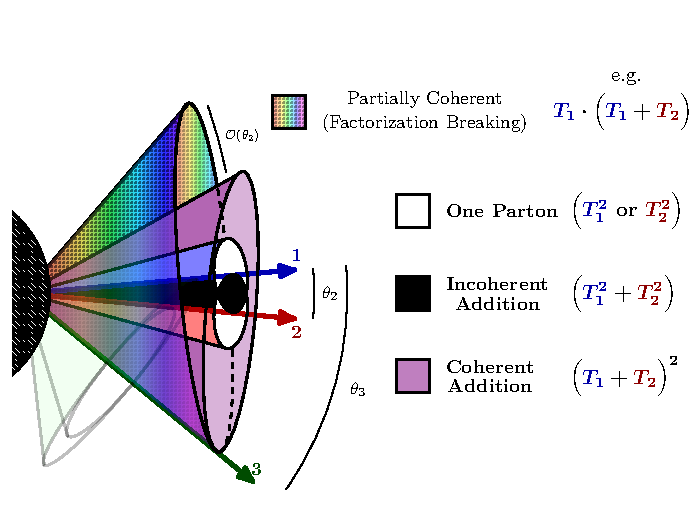
\includegraphics[width=1.05\textwidth]{figures/misc/color_coherence.pdf}
    \caption[A diagram illustrating color coherence and angular ordering in QCD.]
    {
        A diagram illustrating the first stage of color coherence and angular ordering in \gls{qcd}, whose recursive application leads to \Lem{qcd-coherent-branching}.
        %
        Near either individual parton \(i\in\{1,2\}\), soft gluons are emitted with a probability proportional to the \(T_i^2 = C_{R_i}\);
        %
        the overlap in which these probabilities add is striped red and blue.
        %
        However, in the region surrounding \emph{both} partons, indicated in purple, their charges add coherently and soft gluons are emitted with a probability proportional to \(C_{R_1\oplus R_2}\).
        %
        Beyond the collinear limit, a factorization-breaking \emph{fringe} (indicated as rainbow-colored and dotted) emerges around the coherent region, where it is less meaningful to talk about the probability of emitting a soft gluon;
        %
        in this region, the total differential cross section \(\dd\sigma_{N+1}\) \emph{does not factorize} into the product of an \(N\) particle differential cross section \(\dd\sigma_{N}\) and a soft gluon emission probability.
    }
    \label{fig:qcd-coherent-branching}
\end{figure}

\remark{}{
    Notably, \Lem{collinear-color-coherence} reproduces the factor of \(2 C_R \,\, \dd z/z \,\,\dd\theta/\theta\) that we saw emerge with our depth computations of splitting functions from \Secs{collinear-phase-space}{splitting-functions}.
    %
    It is encouraging that the soft limit for our explicit answers for soft gluon emission agree with the result guaranteed by \Thm{soft-gluon}.
    %
    To improve the accuracy of the results we obtain with \Thm{soft-gluon}, we can therefore replace the factor of \(2 C_R \dd \omega / \omega\) by \(P_{ij \leftarrow \ell}(z) \dd z\);
    %
    the splitting functions we derived do not change the behavior of the soft limit above -- any terms they add are subleading to the dominant \(1/z\) term -- but they \emph{also} capture universal behavior of partonic radiation in the purely collinear limit.
}



The tools we have explored in the proof of \Lem{collinear-color-coherence}, and the discussion of its recursion in the QED examples of \Example{charge-coherence} and \Exercise{charge-coherence-mparticle}, give us enough tools to take the next step and make a recursive statement in \gls{qcd}.
%
This may sound intimidating, but is not that bad.
%
Now that we know how the color indices work, everything really behaves structurally similar to the examples in QED -- the new feature is just that when our approximations fail, strict factorization also fails due to color correlations.
%
But we will not consider how.
%
We will pretend (however falsely) that our approximations -- the (recursive) collinear limits we used for coherent branching in QED -- always hold.
%
Now that you are completely absolved of blame for these approximations, I invite you to try the \gls{qcd} calculation yourself -- I really do think it is quite fun.

\begin{exercise}
    \label{ex:qcd-coherent-branching-proof}
    Don't get intimidated by the Lemma below.
    %
    Instead, by following the fixed-order logic of \Lem{collinear-color-coherence} and \Example{charge-coherence}, and the recursive logic of \Exercise{charge-coherence-mparticle} in the limit of a hierarchy of collinear splittings, demonstrate the phenomenon of \vocab{QCD Coherent Branching} (see also \Fig{qcd-coherent-branching}):
\end{exercise}


\begin{lemma}{Coherent Branching}{coherent-branching}
    Consider \(M\) outgoing particles, and an additional soft gluon, in the \vocab{strongly-angular-ordered limit}:%
    \footnote{
        Using the triangle equality, we could also write
        \(
            \theta_{12} \ll \theta_{(12)3} \ll \theta_{(123)4} \ll \cdots
            \,,
        \)
        where \(\theta_{(S)\,\,n}\) is the angle between \(\sum_{i\in S} \vec{k}_i\) and \(\vec{k}_n\).
    }
    \begin{align}
        \theta_{2} \ll \theta_{3} \ll \theta_{4}
        \ll
        \cdots
        \ll
        \theta_M
        \,,
    \end{align}
    where we define \(\theta_j = \theta_{1j}\) to be the angle of particle \(j\) relative to particle 1 for brevity.

    Finally, let \(\theta = \theta_{1q}\) be the angle of the soft gluon relative to particle 1.


    Then, up to terms which vanish in the limit of strong angular ordering, the emission of a soft gluon in a region around particle has the phase space distribution
    \begin{align}
        \label{eq:qcd-coherent-branching}
        \dsigmatilde
        \approx
        4 \as
        \,
        \frac{\dd E_q}{E_q}
        \,
        \frac{\dd \theta_q}{\theta_q}
        \,\,\,
        {\scriptscriptstyle\times}
        \,\,
        \begin{cases}
            C_{R_1}
            & \theta < \theta_{2}
            \\
            C_{R_{(12)}}
            & \theta_{2} \lesssim \theta \lesssim
            \theta_{3}, \theta_{(12)3}
            \\[2ex]
            \quad
            \vdots
            &
            \\[2ex]
            C_{R_{(12\,\cdots\,M-1)}}
            & \theta_{M-1} \lesssim \theta \lesssim
            \theta_{M}, \theta_{(1\cdots M-1)M}
            \,,
        \end{cases}
    \end{align}
    where the \(\lesssim\) is an unambiguous inequality in the strongly-angular-ordered limit, and \(R_{(1\cdots m)} := R_1 \oplus R_2 \oplus \cdots \oplus R_m\) is the representation formed by the direct sum of the representations of particles 1 through \(m\), which has generators (in a tensor product basis)
    \begin{align}
        \le(T^a_{(1\cdots m)}\ri)\indices{^{r_1\,\cdots\,r_m}_{r'_1\,\cdots\,r'_m}}
        \,\,
        :=&
        \,\,
        \le(T^a_{R_1}\ri)\indices{^{r_1}_{r'_1}}
        \,
        \delta\indices{^{r_2}_{r'_2}}\,\cdots\,\delta\indices{^{r_m}_{r'_m}}
        \,\,
        +
        \,\,
        \delta\indices{^{r_1}_{r'_1}}
        \le(T^a_{R_2}\ri)\indices{^{r_2}_{r'_2}}
        \delta\indices{^{r_3}_{r'_3}}\,\cdots\,\delta\indices{^{r_m}_{r'_m}}
        \notag
        \\
        &\qquad
        \,\,
        +
        \,\,
        \cdots
        \,\,
        +
        \delta\indices{^{r_1}_{r'_1}}
        \cdots
        \delta\indices{^{r_{m-1}}_{r'_{m-1}}}
        \le(T^a_{R_m}\ri)\indices{^{r_m}_{r'_m}}
        \,.
    \end{align}
\end{lemma}



We now cool it with the heat.
%
The remainder of the thesis will be less formal and exhausting about foundational results (though I may still advise you take a water break before \Sec{everything-on-shell}).



% ----------------------------------------------
\section{Substructure Diagrams and Fixed-Order Distributions}
% ----------------------------------------------
\label{sec:fixed-order-substructure}

We are finally ready to do some computations which reveal aspects of the internal structure of QCD partons.
%
In this section, we briefly introduce an important calculational tool for our analysis of jet substructure.
%
Before using the results of \Sec{universal-features} to recursively reveal the all-orders structure of jets -- the goal of our next chapter -- we take this opportunity to give results which are valid at \(\mathcal{O}(\alpha_s)\).
%
In \Chap{jets}, we will revisit these computations in the context of \textit{\glspl{jet}}, the beautiful formalism of the partonic cascade in order to obtained \textit{resummed} perturbative predictions which include corrections to arbitrary orders in \(\alpha_s\).


In this thesis, many of the observables we consider will be IRC safe and depend mostly on the less-energetic branch of a partonic splitting, such as mass \glspl{angularity} and \glspl{gecf}.
%
For example, the mass-squared associated with the splitting of a single parton is approximately \(m^2 = z(1-z)(1-\cos\theta) \approx \min(z, 1-z) \theta^2\), since, as shown in \Sec{universal-features}, the phase space of \gls{qcd} is dominated by singularities at which \(z\to 0\) or \(z \to 1\).
%
We call \(\min(z, 1-z)\) the \textit{soft energy fraction}.

The distribution of the angle and soft energy fraction of the splitting of a parton of flavor \(i\) is described in the \gls{collinear-limit} at \(\mathcal{O}(\alpha_s)\) by
%
\begin{align}
    \label{eq:emission-probability}
    \rho_{i}(z,\theta)
    &=
    \frac{\alpha_s}{\pi}
    \le[\bar{p}_i(z)\ri]^{(1/2)}_+ \frac{1}{\theta}
    ,
\end{align}
where \(z\in(0, 1/2)\) and \([\bar{p}(z)]^{(1/2)}_+ = [p(z) + p(1-z)]^{(1/2)}_+\) is a \glslink{plus-fn}{plus-regularized} \gls{redsplitfn}:
%
a modification of the full splitting function encoding only the energy fraction of the softer branch of the splitting.%
\footnote{
   If we would like to deal with observables which do not depend only on the softer energy fraction, we would need to work with a full (\glslink{plus-fn}{plus-regulated}) splitting function \([p(z)]^{(1)}_+\).
}

We will now use our technology to examine the fixed-order behavior of \glspl{observable} involving \textit{jets}.
%
Jets will be discussed in detail in \Chap{jets}, but for now we simply take them to be a collinear configuration of partons with limited angular separation \(\theta < \Rjet\).
%
Using \Eq{emission-probability}, the \(\mathcal{O}(\alpha_s)\) cumulative distribution of an observable \(X\) within a jet initiated by a parton of flavor \(i\) can be quickly represented as
\begin{align}
    \label{eq:cml-fixed-order}
    \Sigma_X(x)
    =
    \int
    \dd \theta
    \,
    \dd z
    \,
    \rho_{i}(z,\theta)
    \,\,
    \Theta(x > X(z, \theta))
    \,
    =
    \,
    \int
    \frac{\dd \theta}{\theta}
    \,
    \frac{\alpha_s}{\pi}
    \,
    \dd z
    \,
    \le[\bar{p}_i(z)\ri]^{(1/2)}_+
    \,
    \frac{\alpha_s}{\pi}
    \,\,
    \Theta(x > X(z, \theta))
    \,,
\end{align}
where we are abusing notation by writing \(X(z, \theta)\) to indicate the observable associated with a pair of momenta separated by an angle \(\theta\) and which carry fractions \(z\) and \((1-z)\) of the momenta of the full jet.


The definition of \glslink{plus-fn}{plus-regularization} yields
\begin{align}
    \int_0^{1/2} \dd z \le[\bar{p}(z)\ri]^{(1/2)}_+ g(z)
    =
    \int_0^{1/2} \dd z \,\, \bar{p}(z) \le(g(z) - g(0)\ri)
    \,,
\end{align}
assuming (correctly) that \(p(z)\) is only singular when \(z = 0\).
%
\begin{subequations}
Using also that \(\Theta(a) = 1 - \Theta(-a)\), we can therefore re-write \Eq{cml-fixed-order} as
\begin{align}
    \Sigma_X(x)
    \,
    &=
    \,
    \int
    \frac{\dd \theta}{\theta}
    \,
    \dd z
    \,
    \le[\bar{p}_i(z)\ri]^{(1/2)}_+
    \,
    \frac{\alpha_s}{\pi}
    \,\,
    \le(
        1 - \Theta(X(z, \theta) > x)
    \ri)
    \\
    &=
    \,
    \int
    \frac{\dd \theta}{\theta}
    \,
    \dd z
    \,
    \bar{p}_i(z)
    \,
    \frac{\alpha_s}{\pi}
    \,\,
    \le(
        -\Theta(X(z, \theta) > x)
        +\Theta(X(0, \theta) > x)
    \ri)
    \,.
\end{align}
%
The observables we consider in this thesis, such as masses and angularities, have \(X\big|_{z=0} = 0\), so that \(X(0, \theta) < x\) for any finite \(x\)
%
Therefore, we may write, at least for \(x > 0\), that
\begin{align}
    \label{eq:cml-fixed-order-veto}
    \Sigma_X(x)
    \,
    &=
    \,
    -
    \int
    \frac{\dd \theta}{\theta}
    \,
    \dd z
    \,
    \bar{p}_i(z)
    \,
    \frac{\alpha_s}{\pi}
    \,\,
    \Theta(X(z, \theta) > x)
    \,.
\end{align}
%
\end{subequations}


\remark{}{
    The region of phase space in which an emission contributes a value greater than \(x\) to the observable \(X\) -- i.e. where \(X(z, \theta) > x\) -- is called a \vocab{\gls{vetoreg}}.
    %
    \Eq{cml-fixed-order-veto} therefore expresses the cumulative distribution for \(X\) as the integral of the phase space density \(\rho_i(z, \theta)\) over the veto region.
    %
    The integral of \(\rho_i(z,\theta)\) over the \gls{vetoreg} for an observable is also called the \vocab{\gls{radiator}} \(R_X(x)\) for the observable.
    %
    The radiator will reappear in our calculations of resummed quantities in \Chap{jets}, and modified definitions will even capture the effects of multiple emissions and the running coupling of QCD.
}


The integral of \Eq{cml-fixed-order} captures the probability that a jet contains a single emission which lies in a particular region of phase space.
%
We will represent such integrals in terms of \vocab{\glspl{substructure-diagram}}:

\begin{definitionbox}{Substructure Diagram}{substructure-diagram}
    A \emph{\gls{substructure-diagram}} is a graphical representation that the probability of a splitting whose angle \(\theta\) and softer energy fraction \(z\) lie within some region of phase space.

    \vspace{7pt}
    \hrule
    \vspace{7pt}

    \vocab{Substructure diagrams} describe the probability of finding a splitting in some region in the \(\log(z^{-1})\)-\(\log(\theta^{-1})\) plane, or Lund plane, with a diagram of the Lund plane with the corresponding region filled:
%
\begin{align}
    \iint_{
    \begin{tikzpicture}[scale=.06]
    \begin{axis}
    [xmin=0, xmax=5,
    ymin=0, ymax=5,
    axis line style = {draw=none},
    ticks=none]
    	\draw[blue, line width=9pt, fill=blue,fill opacity=0.3] \pgfextra{
    	  \pgfpathellipse{\pgfplotspointaxisxy{2.5}{2.5}}
    		{\pgfplotspointaxisdirectionxy{0}{1.8}}
        	{\pgfplotspointaxisdirectionxy{1.2}{.5}}
    	};
    \end{axis}
    \end{tikzpicture}
    }
    \frac{\alpha_s}{\pi}~
    \frac{\dd\theta}{\theta}~
    \dd z~
    [\bar{p}_i(z)]^{(1/2)}_+
    ~~~
    \triangleq
    ~~~
    \begin{tikzpicture}[
    baseline={([yshift=-.8ex]current bounding box.center)},
    vertex/.style={anchor=base,
    circle,fill=black!25,minimum size=18pt,inner sep=2pt},
    scale=.3]
    \begin{axis}
    [
    xlabel=\scalebox{2.5}
    {\(\log(\theta^{-1})\)},
    ylabel=\scalebox{2.5}
    {\(\log(z^{-1})\)},
    xmin=0, xmax=5,
    ymin=0, ymax=5,
    axis line style = {line width=3pt},
    axis y line*=left,
    axis x line*=bottom,
    axis lines = middle,
    ticks=none]
    	\draw[blue, line width=3pt, fill=blue,fill opacity=0.3]
    	\pgfextra{
    	  \pgfpathellipse{\pgfplotspointaxisxy{1.1}{1.6}}
    		{\pgfplotspointaxisdirectionxy{-.2}{.9}}
    		{\pgfplotspointaxisdirectionxy{.7}{.5}}
    	};
    \end{axis}
    \end{tikzpicture}
    ~~~
    \triangleq
    ~~~
    \begin{tikzpicture}[
    baseline={([yshift=-.8ex]current bounding box.center)},
    vertex/.style={anchor=base,
    circle,fill=black!25,minimum size=18pt,inner sep=2pt},
    scale=.3]
    \begin{axis}
    [xmin=0, xmax=5,
    ymin=0, ymax=5,
    axis line style = {line width=3pt},
    axis y line*=left,
    axis x line*=bottom,
    axis lines = middle,
    ticks=none]
    	\draw[blue, line width=3pt, fill=blue,fill opacity=0.3]
    	\pgfextra{
    	  \pgfpathellipse{\pgfplotspointaxisxy{1.1}{1.6}}
    		{\pgfplotspointaxisdirectionxy{-.2}{.9}}
    		{\pgfplotspointaxisdirectionxy{.7}{.5}}
    	};
    \end{axis}
    \end{tikzpicture}
    ,
\end{align}
where the shaded oval in the Lund plane above represents an arbitrary shape associated with a region of two-particle phase space.
\end{definitionbox}


\remark{}{
It follows, for example, that
%
\begin{align}
    \label{eq:plus-fn-diagram-identities}
    \begin{tikzpicture}[
    baseline={([yshift=-.8ex]current bounding box.center)},
    vertex/.style={anchor=base,
    circle,fill=black!25,minimum size=18pt,inner sep=2pt},
    scale=.3]
    \begin{axis}
    [xmin=0, xmax=5,
    ymin=0, ymax=5,
    axis line style = {line width=3pt},
    axis y line*=left,
    axis x line*=bottom,
    axis lines = middle,
    ticks=none]
    	\draw[blue, line width=3pt, fill=blue,fill opacity=0.3]
    	\pgfextra{
    	  \pgfpathellipse{\pgfplotspointaxisxy{0}{0}}
    		{\pgfplotspointaxisdirectionxy{0}{100}}
    		{\pgfplotspointaxisdirectionxy{100}{0}}
    	};
    \end{axis}
    \end{tikzpicture}
    =
    0
    ~~~~~~~~~
    {\rm and}
    ~~~~~~~~~
    \begin{tikzpicture}[
    baseline={([yshift=-.8ex]current bounding box.center)},
    vertex/.style={anchor=base,
    circle,fill=black!25,minimum size=18pt,inner sep=2pt},
    scale=.3]
    \begin{axis}
    [xmin=0, xmax=5,
    ymin=0, ymax=5,
    axis line style = {line width=3pt},
    axis y line*=left,
    axis x line*=bottom,
    axis lines = middle,
    ticks=none]
    	\draw[blue, line width=3pt, fill=blue,fill opacity=0.3]
    	\pgfextra{
    	  \pgfpathellipse{\pgfplotspointaxisxy{0}{0}}
    		{\pgfplotspointaxisdirectionxy{0}{100}}
    		{\pgfplotspointaxisdirectionxy{100}{0}}
    	};
    	\draw[blue, line width=3pt, fill=white,fill opacity=1.0]
    	\pgfextra{
    	  \pgfpathellipse{\pgfplotspointaxisxy{1.1}{1.6}}
    		{\pgfplotspointaxisdirectionxy{-.2}{.9}}
    		{\pgfplotspointaxisdirectionxy{.7}{.5}}
    	};
    \end{axis}
    \end{tikzpicture}
    ~~
    =
    ~~
    \begin{tikzpicture}[
    baseline={([yshift=-.8ex]current bounding box.center)},
    vertex/.style={anchor=base,
    circle,fill=black!25,minimum size=18pt,inner sep=2pt},
    scale=.3]
    \begin{axis}
    [xmin=0, xmax=5,
    ymin=0, ymax=5,
    axis line style = {line width=3pt},
    axis y line*=left,
    axis x line*=bottom,
    axis lines = middle,
    ticks=none]
    	\draw[blue, line width=3pt, fill=blue,fill opacity=0.3]
    	\pgfextra{
    	  \pgfpathellipse{\pgfplotspointaxisxy{0}{.9}}
    		{\pgfplotspointaxisdirectionxy{0}{200}}
    		{\pgfplotspointaxisdirectionxy{2.5}{.9}}
    	};
    	\draw[blue, line width=3pt, fill=white,fill opacity=1.0]
    	\pgfextra{
    	  \pgfpathellipse{\pgfplotspointaxisxy{1.1}{1.6}}
    		{\pgfplotspointaxisdirectionxy{-.2}{.9}}
    		{\pgfplotspointaxisdirectionxy{.7}{.5}}
    	};
    \end{axis}
    \end{tikzpicture}
    ~~
    =
    ~~
    -~
    \begin{tikzpicture}[
    baseline={([yshift=-.8ex]current bounding box.center)},
    vertex/.style={anchor=base,
    circle,fill=black!25,minimum size=18pt,inner sep=2pt},
    scale=.3]
    \begin{axis}
    [xmin=0, xmax=5,
    ymin=0, ymax=5,
    axis line style = {line width=3pt},
    axis y line*=left,
    axis x line*=bottom,
    axis lines = middle,
    ticks=none]
    	\draw[blue, line width=3pt, fill=blue,fill opacity=0.3]
    	\pgfextra{
    	  \pgfpathellipse{\pgfplotspointaxisxy{1.1}{1.6}}
    		{\pgfplotspointaxisdirectionxy{-.2}{.9}}
    		{\pgfplotspointaxisdirectionxy{.7}{.5}}
    	};
    \end{axis}
    \end{tikzpicture}
    .
\end{align}
As depicted above, we may replace any vertical line -- representing an integral over \(z\) at fixed \(\theta\) -- or any vertical strip -- representing an integral over \(z\) and some range of \(\theta\) -- with zero, since the integral of a \gls{plus-fn} is zero.
}



\begin{example}
    \label{ex:mass-fixed-order}
    The pairwise mass of two massless partons emerging from a single splitting is given by
    \begin{equation}
    \begin{aligned}
        m^2 &= (p_1 + p_2)^2 = 2 p_1 \cdot p_2
        =
        2 Q^2
        \,
        z \, (1-z)
        \le(1 - \cos(\theta)\ri)
        \\
        &\approx
        Q^2 z \theta^2
        .
    \end{aligned}
    \end{equation}

    Therefore, in a jet of radius \(\Rjet\), the corresponding \gls{substructure-diagram} showing the veto region \(z\theta^2 > m^2 / Q^2\) is
    \begin{center}
    \begin{tikzpicture}[scale=0.5]
    \begin{axis}
    [xlabel=\(\log(\theta^{-1})\), ylabel=\(\log(z^{-1})\),
    xmin=0, xmax=5,
    ymin=0, ymax=5,
    axis line style = very thick,
    axis y line*=left,
    axis x line*=bottom,
    axis lines = middle,
    ticks=none]
        \addplot[name path=f,domain=0:5,
        style=very thick,blue]
        {4.5-1.5*x};

        \path[name path=axis]
        (axis cs:0,0) -- (axis cs:1,0);

        \addplot [
            thick,
            color=blue,
            fill=blue,
            fill opacity=0.3
        ]
        fill between[
            of=f and axis
        ];

        \node [rotate=-50] at (axis cs:  2.2,  2.3) {$m^2 = z\theta^2$};
    \end{axis}
    \end{tikzpicture}
    \end{center}

    We can easily read off the resummed distribution for the mass squared of a jet at the level of accuracy we are pursuing (leaving the integrals to you):
    \begin{align}
        \Sigma(m^2)
        \approx
        -
        \,\,\,
        \raisebox{-10pt}{
        \begin{tikzpicture}[
        baseline={([yshift=-.8ex]current bounding box.center)},
        vertex/.style={anchor=base,
        circle,fill=black!25,minimum size=18pt,inner sep=2pt},
        scale=.3]
        \begin{axis}
        [xmin=0, xmax=5,
        ymin=0, ymax=5,
        axis line style = very thick,
        axis y line*=left,
        axis x line*=bottom,
        axis lines = middle,
        ticks=none]
        	\addplot[name path=f,domain=0:5,
            style=very thick,blue]
            {4.5-1.5*x};
            \path[name path=axis]
            (axis cs:0,0) -- (axis cs:1,0);
            \addplot [
                thick,
                color=blue,
                fill=blue,
                fill opacity=0.3
            ]
            fill between[
                of=f and axis
            ];
        \end{axis}
        \end{tikzpicture}
        }
        =
        -
        \frac{\alpha_{\rm S}}{\pi}
        \iint_{z\theta^2 > m^2}
        \dd\log(\theta) ~~ \dd z ~ [p(z)]_+
    \end{align}

    Plugging in the leading, singular piece for the splitting function at leading logarithmic accuracy, \(p(z) \sim 2 C_R / z\) for a splitting initiated by a parton with \(SU(3)\) color representation \(R\), and putting back in factors of \(Q\), we find
    \begin{align}
        \Sigma(m^2)
        \approx
        -\frac{C_R\alpha_{\rm S}}{2 \pi}\log^2\left(\frac{m^2}{Q^2}\right)
        \,,
    \end{align}
    with the associated pseudo-probability density
    \begin{align}
        \rho(m^2)
        =
        \frac{\dd}{\dd m^2} \Sigma(m^2)
        \approx
        \frac{C_R \alpha_s}{\pi}
        \frac{1}{m^2}
        \log\le(\frac{Q^2}{m^2}\ri)
        \,.
    \end{align}

    This describes the mass-squared distribution for a two-particle final state in the \gls{collinear-limit}.
    %
    We will include the effects of many emissions in \Sec{ll-substructure-diagrams} of \Chap{jets}.
\end{example}
~\\

\begin{exercise}{}
    Repeat the analysis of Example \ref{ex:mass-fixed-order} above with and without \glspl{substructure-diagram} for the leading pieces of the NLO distributions of \glspl{angularity} \(e_\varsigma\) (\Eq{angularitydefn_lo}) and \glspl{gecf} \(C_1^{(\varsigma)}\) (\Eq{GECFdefn_lo}).
    %
    I find
    \begin{align}
        \Sigma_{\le(e_\varsigma\ri)}(x)
        \approx
        \Sigma_{\le(C_1^{(\varsigma)}\ri)}(x)
        \,\,
        &\approx
        \,\,
        -\frac{C_R\alpha_{\rm S}}{\varsigma \pi}\log^2(x)
        \\
        \rho_{\le(e_\varsigma\ri)}(x)
        \approx
        \rho_{\le(C_1^{(\varsigma)}\ri)}(x)
        \,\,
        &\approx
        \,\,
        -\frac{C_R\alpha_{\rm S}}{\varsigma \pi} \frac{1}{x}
        \log\left(x\right)
        \,.
    \end{align}
    Compare these two results to the mass distribution of a partonic splitting obtained in \Example{mass-fixed-order}.

    Argue that all three may be plus-regularized (as discussed in the context of splitting functions in \Sec{splitting-functions}) to yield a normalized distribution, though not a probability distribution.
\end{exercise}




% ==============================================
\section{Connecting back out}
% ==============================================

In this chapter, we have explored the framework of scattering and quantum field theory used by particle physicists to explore the subatomic universe.
%
Our discussions and derivations of the universal, fixed-order features of \gls{qcd} gave us quantitative tests of \gls{qcd} scattering.
%
We saw a hint of something deeper, however:
%
we may hope to push beyond fixed order predictions by repeated application of soft theorems and angular ordering.
%
We pursue a more rigorous understanding of this recursive, fractal-like nature of \gls{qcd} radiation in the next chapter, where we will discover and quantify the intricate features of jets.



\begin{subappendices}

\section{A Collinear QCD Compendium}
\label{app:qcd-compendium}

\subsection{Gluons and Polarization Vectors}

Polarization vectors are a tricky business -- the transformation properties of polarizations are inextricably linked with gauge invariance.%
\footnote{
    see Weinberg's \underline{The Theory of Quantum Fields, Volume I}, Chapter 2.5 \cite{Weinberg:1995mt} and especially Matthew Schwartz' \underline{Quantum Field Theory and the Standard Model}, Chapter 8.4.2 \cite{Schwartz:2014sze}.
}
%
As we saw in \Sec{splitting-functions}, where Ward identities did not apply, we have to be careful in computations with off-shell legs, and the mixing of the properties of polarizations and gauge-invariance can be confusing.

However, we can pick convenient bases for the physical polarization vectors of gluons.
%
For a spin-one gauge boson moving along the \(z\)-axis, \(p^\mu - E_p \le(1,0,0,1\ri)\), a canonical basis for the polarization vectors is the pair
\begin{subequations}
\label{eq:z-polarization}
\begin{align}
    \varepsilon^\mu_{+,\,z}
    &\reppedby
    \frac{1}{\sqrt{2}}
    \le(0, 1, -i, 0\ri)
    \\
    \varepsilon^\mu_{-,\,z}
    &\reppedby
    \frac{1}{\sqrt{2}}
    \le(0, 1, +i, 0\ri)
    \,,
\end{align}
\end{subequations}
with the notable property that
\begin{align}
    \varepsilon_\lambda \cdot \varepsilon_{\lambda'}^*
    =
    \delta_{\lambda \lambda'}
    \,.
\end{align}


\begin{exercise}
    Show that \(p\cdot \epsilon = 0\) for the polarization four-vectors of \Eq{z-polarization}, and furthermore that they are eigenvectors of the \textit{little group transformations} -- Lorentz transformations which leave the momentum \(p^\mu\) invariant -- consisting of rotations about the \(z\)-axis represented by the matrix \(\Lambda(\phi)\)%
    \footnote{
        These rotations are not the only little group transformations for our massless gluon, but they are the only ones that matter;
        %
        see Weinberg's \underline{The Theory of Quantum Fields, Volume I}, Chapter 2.5 \cite{Weinberg:1995mt}.
    }:
    \begin{align}
        \Lambda\indices{^\mu_\nu}(\phi) \varepsilon^\nu_{\pm,\,z}
        =
        e^{\pm i \phi} \varepsilon^\mu_{\pm,\,z}
        \,.
    \end{align}
\end{exercise}



A constructive way of producing polarization vectors for general momenta is by selecting two arbitrary four-vectors, projecting each to the component orthogonal to the gauge-boson four-momentum \(p^\mu\) (Mathematica's \texttt{Orthogonalize} is a useful tool), and then finding the orthogonal linear combinations which are eigenvectors of the little group rotations of \(p^\mu\).
%
For the calculations of splitting functions in this section,
%(and for the calculation of the QED polarization vectors in \Prob{massless-qed}),
we now record the results for polarization vectors of collinear gluons.

\begin{example}
In the concrete calculations of splitting functions in \Sec{splitting-functions}, we will also need polarization vectors for \textit{collinear} gluons travelling nearly along the \(z\)-axis, with a polar angle \(\theta \ll 1\):
\begin{align}
    k^\mu =
    E_k
    \le(1,\, \sin\theta\cos\phi,\, \sin\theta\sin\phi,\,\cos\theta\ri)
    =
    E_k
    \le(1,\, \theta\cos\phi,\, \theta\sin\phi,\,1 - \theta^2/2\ri)
    +
    \mathcal{O}(\theta^3)
    \,.
\end{align}
A convenient basis for the associated polarization vectors in our collinear limit calculations is
\begin{align}
    \label{eq:collinear-polarization}
    \varepsilon^\mu_\lambda(k)
    \approx
    \varepsilon^\mu_\lambda
    -
    \frac{e^{-i\lambda \phi}}{\sqrt{2}}
    \le(
    \frac{\theta^2}{2}\cos\phi,\,
    \frac{\theta^2}{2}\sin\phi,\,
    \theta
    \ri)
    \,,
\end{align}
where \(\lambda \in \{+,-\}\).
\end{example}

\begin{exercise}
    Show that the collinear-limit polarization vectors of \Eq{collinear-polarization} are orthogonal to the collinear momentum \(k^\mu\) and are mutually orthonormal, at \(\mathcal{O}(\theta^2)\).
\end{exercise}




\subsection{Quarks and Polarization Bi-Spinors}

A full Lorentz- and parity-invariant description of fermions in \(d = 3+1\) dimensions requires the use of \textit{gamma matrices}, satisfying
\begin{align}
    \acomm{\gamma^\mu}{\gamma^\nu} = -2 g^{\mu\nu}
    \,.
\end{align}
%
In the concrete calculations of this work, we will use the \textit{chiral} basis for the gamma matrices:
\begin{align}
    \gamma^\mu = \pmtrx{0 & \sigma^\mu\\\overline{\sigma}^\mu & 0}
    \,,
\end{align}
where \(\sigma^\mu = (1, \vec{\sigma})\) and \(\overline{\sigma}^\mu = (1, -\vec{\sigma})\) are invariant symbols of the Lorentz group.


\begin{example}
    \label{ex:collinear-kslash}
    Consider a massless particle with momentum \(k_1^\mu\) moving at a polar angle \(\theta_1\) relative to the \(z\) axis and an azimuthal angle \(\phi_1\) in the \(x\)-\(y\) plane.
    %
    Its momentum is \(k^\mu \reppedby E_1 \le(1, \sin\theta_1\cos\phi_1, \sin\theta_1 \sin\phi_1,\cos\theta_1\ri)\), and therefore
    \begin{align}
        \slashed{k}_1
        :=
        k_1^\mu \gamma_\mu
        &=
        E_1 \pmtrx{0 & 1 - \vec{k}\cdot \vec{\sigma} \\ 1 +  \vec{k}\cdot \vec{\sigma} & 0}
        \\
        &=
        E_1
        \pmtrx{
            0&0&1 - \cos\theta_1& -\sin\theta_1 e^{-i\phi_1}
            \\
            0&0& -\sin\theta_1 e^{i\phi_1} & 1 + \cos\theta_1
            \\
            1 + \cos\theta_1 & \sin\theta_1 e^{-i\phi_1} & 0 & 0
            \\
            \sin\theta_1 e^{i\phi_1} & 1 - \cos\theta_1 & 0 & 0
        }
        \,.
    \end{align}
    In the collinear limit where \(\theta_1 \ll 1\), as we often consider in this thesis, we can therefore write
    \begin{align}
        \slashed{k}_1
        =
        E_1
        \pmtrx{
            0&0& \theta_1^2/2 & -\theta_1 e^{-i\phi_1}
            \\
            0&0 & -\theta_1 e^{i\phi_1} & 2 - \theta_1^2/2
            \\
            2 - \theta_1^2/2 & \theta_1 e^{-i\phi_1} & 0 & 0
            \\
            \theta_1 e^{i \phi_1} & \theta_1^2/2 & 0 & 0
        }
        +
        \mathcal{O}\le(\theta_1^3\ri)
        \,.
    \end{align}
    This expression is useful for several of the concrete computations of this chapter.
\end{example}



In this basis, spinor factors take the form
\begin{subequations}
\begin{align}
    \label{eq:bispinor-u}
    u_s(p)
    &=
    \pmtrx{
        \sqrt{p\cdot \sigma}\ket{s}
        \\
        \sqrt{p\cdot{\overline{\sigma}}} \ket{s}
    }
    \\
    \label{eq:bispinor-v}
    v_s(p)
    &=
    \pmtrx{
        \sqrt{p\cdot \sigma}\sigma_x \ket{s}
        \\
        -\sqrt{p\cdot{\overline{\sigma}}} \sigma_x \ket{s}
    }
    =:
    \pmtrx{
        \sqrt{p\cdot \sigma}\ket{\overline{s}}
        \\
        -\sqrt{p\cdot{\overline{\sigma}}} \ket{\overline{s}}
    }
    \,,
\end{align}
\end{subequations}
where we have abused notation by using \(\ket{s}\) to denote the 2-spinor encoding the particle's spin measured in the \(\sigma_z\)/``computational'' basis.
%
In particular
\begin{align}
    \ket{s}
    =
    \begin{cases}
        \pmtrx{1\\0}
        &
        s = +
        \quad \leftrightarrow \quad
        \text{spin } s \text{ is along } +\hat{z}
        \,,
        \\
        \pmtrx{0\\1}
        &
        s = -
        \quad \leftrightarrow \quad
        \text{spin } s \text{ is along } -\hat{z}
        \,.
    \end{cases}
\end{align}

For a four-component spinor \(\psi\) (such as \(u_s(p)\) or \(v_s(p)\)) \(\bar{\psi}\) is defined by
\begin{align}
    \bar{\psi} := \psi^\dagger \gamma^0
    \,,
\end{align}


\begin{example}
    \label{eq:massive-bispinor}
    Consider a massive spin-1/2 particle moving in the \(z\)-direction with energy \(E_P\) and momentum \(\vec{P} = P \hat{z}\) along the \(z\)-axis.
    %
    Using our suboptimal metric signature (\(g = \text{diag}(+,-,-,-)\)), we have
    \begin{align}
        p\cdot \sigma
        =
        \pmtrx{E_P - P & 0 \\ 0 & E_P + P}
        =:
        E_P \pmtrx{1 - \beta & 0 \\ 0 & 1 + \beta}
        \\
        p\cdot \overline{\sigma}
        =
        \pmtrx{E_P + P & 0 \\ 0 & E_P - P}
        =:
        E_P \pmtrx{1 + \beta & 0 \\ 0 & 1 - \beta}
        \,,
    \end{align}
    where \(\beta := P / E_P\) is the velocity of the particle;
    %
    we also have \(\beta^2 = 1 - m^2/E^2\).

    Therefore, using the Weyl basis for the gamma matrices, we may write
    \begin{align}
        \label{eq:bispinor-u-virtual}
        u_+(P)
        =
        \sqrt{E_P}
        \pmtrx{\sqrt{1-\beta}\\0\\\sqrt{1+\beta}\\0}
        \,,\qquad
        u_-(P)
        =
        \sqrt{E_P}
        \pmtrx{0\\\sqrt{1+\beta}\\0\\\sqrt{1-\beta}}
        \,,
        \\
        \label{eq:bispinor-v-virtual}
        v_+(P)
        =
        \sqrt{E_P}
        \pmtrx{0\\\sqrt{1+\beta}\\0\\-\sqrt{1-\beta}}
        \,,\qquad
        v_-(P)
        =
        \sqrt{E_P}
        \pmtrx{\sqrt{1-\beta}\\0\\-\sqrt{1+\beta}\\0}
        \,.
    \end{align}

    % In the high-energy limit \(\beta \approx 1 - m^2 / 2 E^2\), and
    % \begin{align}
    %     \label{eq:bispinor-u-high-energy}
    %     u_+(P)
    %     =
    %     \sqrt{2E_P}
    %     \pmtrx{m / 2 E_P \\0\\1\\0}
    %     ,\qquad
    %     u_-(P)
    %     =
    %     \sqrt{2 E_P}
    %     \pmtrx{0 \\ 1 \\0\\m / 2 E_P}
    %     \,,
    %     \\
    %     \label{eq:bispinor-v-high-energy}
    %     v_+(P)
    %     =
    %     \sqrt{2 E_P}
    %     \pmtrx{0\\1\\0\\-m/2E_P}
    %     ,\qquad
    %     v_-(P)
    %     =
    %     \sqrt{2 E_P}
    %     \pmtrx{m/2E_P\\0\\-1\\0}
    %     \,,
    % \end{align}
    % up to \(\mathcal{O}\le(\frac{m^2}{E^2}\ri)\) (approximation is instructive, but dropping these terms drops important e
\end{example}



\begin{exercise}
    Using \Eqs{bispinor-u}{bispinor-v}, show that \(\sum_s u_s(p) \bar{u}_s(p) = \slashed{p} + m\), and \(\sum_s v_s(p) \bar{v}_s(p) = \slashed{p} - m\).

    \vspace{7pt}
    \hrule

    \begin{center}
        \texttt{(Hint:)}

        Use \(\sum_s \ketbra{s}{s} = 1\).
    \end{center}
\end{exercise}



At high energies, or in the massless limit, the polarization bi-spinors take the form
\begin{subequations}
\label{eq:massless-four-component-spinors}
\begin{align}
    u_s(p)
    &=
    \sqrt{\frac{E_p}{2}}
    \pmtrx{
        \le(1 - \hat{p}\cdot \vec{\sigma}\ri)\ket{s}
        \\
        \le(1 + \hat{p}\cdot \vec{\sigma}\ri)\ket{s}
    }
    \\
    v_s(p)
    &=
    \sqrt{\frac{E_p}{2}}
    \pmtrx{
        \le(1 - \hat{p}\cdot \vec{\sigma}\ri) \ket{\overline{s}}
        \\
        -\le(1 + \hat{p}\cdot \vec{\sigma}\ri) \ket{\overline{s}}
    }
    \,,
\end{align}
where \(E_p = p^0\).
\end{subequations}

We note also that
\begin{align}
    \hat{p}\cdot\vec{\sigma}
    =
    \pmtrx{
        \cos\theta            &    \sin\theta e^{-i\phi}
        \\
        \sin\theta e^{i\phi}  &    -\cos\theta
    }
    \,,
\end{align}
where \(\theta\) is the polar angle of \(\hat{p}\) relative to the \(z\)-axis.



\begin{exercise}
    Verify \Eq{massless-four-component-spinors}.
    %
    Show that it implies \(\sum_s u_s \bar{u}_s = \sum_s v_s \bar{v}_s = \slashed{p}\).
\end{exercise}


\begin{example}
    \label{ex:collinear-bispinor}
    Finally, we take the limit in which a massless particle is nearly \glslink{collinear-limit}{collinear} with the \(z\)-axis, for which
    %
    \(
        p^\mu
        =
        E \le(1, \, \sin\theta \cos\phi, \, \sin\theta \sin\phi, \, \cos\theta\ri)
    \)
    %
    reduces to
    %
    \(
        p^\mu
        =
        E \le(1, \, \theta \cos\phi, \, \theta\sin\phi, \, 1 - \theta^2/2\ri)
        +
        \mathcal{O}(\theta^3)
    \).
    %
    In this limit, we have
    \begin{align}
        \hat{p}\cdot\vec{\sigma}
        \approx
        \pmtrx{1 - \theta^2/2& \theta e^{-i\phi} \\ \theta e^{i\phi} & -1+\theta^2/2}
        +
        \mathcal{O}(\theta^3)
        \,,
    \end{align}
    and accordingly, at \(\mathcal{O}(\theta^2)\),
    \begin{align}
        \label{eq:bispinor-u-collinear}
        u_+(p)
        =
        \sqrt{2 E_p}
        \pmtrx{\theta^2/4 \\ -\theta e^{i\phi}/2 \\ 1-\theta^2/4 \\ \theta e^{i\phi}/2}
        +
        \mathcal{O}(\theta^3)
        \,,
        \quad
        u_-(p)
        =
        \sqrt{2 E_p}
        \pmtrx{-\theta e^{-i\phi}/2 \\ 1 - \theta^2/4\\ \theta e^{-i\phi}/2 \\  \theta^2/4}
        +
        \mathcal{O}(\theta^3)
        \,,
        \\
        \label{eq:bispinor-v-collinear}
        v_+(p)
        =
        \sqrt{2 E_p}
        \pmtrx{-\theta e^{-i\phi}/2 \\ 1 - \theta^2/4\\ -\theta e^{-i\phi}/2 \\ -\theta^2/4}
        +
        \mathcal{O}(\theta^3)
        \,,
        \quad
        v_-(p)
        =
        \sqrt{2 E_p}
        \pmtrx{\theta^2/4\\ -\theta e^{i\phi}/2 \\ -1+\theta^2/4 \\ -\theta e^{i\phi}/2}
        +
        \mathcal{O}(\theta^3)
        \,.
    \end{align}
\end{example}


\begin{exercise}
    Verify that \(\sum_s u_s \bar{u}_s (p) = \sum_s v_s \bar{v}_s (p) = \slashed{p}\) at \(\mathcal{O}(\theta^2)\) for the collinear spinors above.
    % \Eqs{bispinor-square-u}{bispinor-square-v}.
    % Working to \(\mathcal{O}(\theta)\) for brevity, verify that
    % \begin{align}
    %     u_+\bar{u}_+(p)
    %     &=
    %     2 E_p
    %     \pmtrx{
    %         0 & 0 & 0 & 0 \\
    %         -\frac{1}{2} \theta  e^{i \phi } & 0 & 0 & 0 \\
    %         1 & \frac{1}{2} \theta  e^{-i \phi } & 0 &
    %         -\frac{1}{2} \theta  e^{-i \phi } \\
    %         \frac{1}{2} \theta  e^{i \phi } & 0 & 0 & 0
    %     }
    %     +
    %     \mathcal{O}(\theta^2)
    %     \,,
    %     \\
    %     u_-\bar{u}_-(p)
    %     &=
    %     2 E_p
    %     \pmtrx{
    %         0 & 0 & 0 & -\frac{1}{2} \theta  e^{-i \phi } \\
    %         \frac{1}{2} \theta  e^{i \phi } & 0 &
    %         -\frac{1}{2} \theta  e^{i \phi } & 1 \\
    %         0 & 0 & 0 & \frac{1}{2} \theta  e^{-i \phi } \\
    %         0 & 0 & 0 & 0
    %     }
    %     +
    %     \mathcal{O}(\theta^2)
    %     \,,
    %     \\
    %     v_+\bar{v}_+(p)
    %     &=
    %     \pmtrx{
    %         0 & 0 & 0 & -\frac{1}{2} \theta  e^{-i \phi } \\
    %         -\frac{1}{2} \theta  e^{i \phi } & 0 &
    %         -\frac{1}{2} \theta  e^{i \phi } & 1 \\
    %         0 & 0 & 0 & -\frac{1}{2} \theta  e^{-i \phi } \\
    %         0 & 0 & 0 & 0
    %     }
    %     +
    %     \mathcal{O}\le(\theta^2\ri)
    %     \,,
    %     \\
    %     v_-\bar{v}_-(p)
    %     &=
    %     \pmtrx{
    %         0 & 0 & 0 & 0 \\
    %         \frac{1}{2} \theta  e^{i \phi } & 0 & 0 & 0 \\
    %         1 & \frac{1}{2} \theta  e^{-i \phi } & 0 &
    %         \frac{1}{2} \theta  e^{-i \phi } \\
    %         \frac{1}{2} \theta  e^{i \phi } & 0 & 0 & 0 \\
    %         \frac{1}{2} \theta  e^{i \phi } & 0 & 0 & 0
    %     }
    %     +
    %     \mathcal{O}\le(\theta^2\ri)
    %     \,.
    % \end{align}

    % Checking terms to \(\mathcal{O}(\theta^2)\) (though higher-order terms agree as well), we find
    % \begin{align}
    %     \label{eq:bispinor-square-u}
    %     \sum_s u_s \bar{u}_s (p)
    %     &
    %     =
    %     2 E_p
    %     \pmtrx{
    %         0 & 0 & 0 & -\frac{1}{2} \theta  e^{-i \phi } \\
    %         0 & 0 & -\frac{1}{2} \theta  e^{i \phi } & 1 \\
    %         1 & \frac{1}{2} \theta  e^{-i \phi } & 0 & 0 \\
    %         \frac{1}{2} \theta  e^{i \phi } & 0 & 0 & 0
    %     }
    %     +
    %     \mathcal{O}\le(\theta^2\ri)
    %     \overset{\checkmark}{=}
    %     \slashed{p}
    %     \\
    %     \label{eq:bispinor-square-v}
    %     \sum_s v_s \bar{v}_s (p)
    %     &
    %     =
    %     2 E_p
    %     \pmtrx{
    %         0 & 0 & 0 & -\frac{1}{2} \theta  e^{-i \phi } \\
    %         0 & 0 & -\frac{1}{2} \theta  e^{i \phi } & 1 \\
    %         1 & \frac{1}{2} \theta  e^{-i \phi } & 0 & 0 \\
    %         \frac{1}{2} \theta  e^{i \phi } & 0 & 0 & 0
    %     }
    %     +
    %     \mathcal{O}\le(\theta^2\ri)
    %     \overset{\checkmark}{=}
    %     \slashed{p}
    %     \,,
    % \end{align}
    % agreeing with the \(\mathcal{O}\le(\theta\ri)\) expansion of \Example{collinear-kslash} (and higher, if we wrote more).
\end{exercise}




\subsection{Color Factors and SU(3)}

\begin{subequations}
The \(T_F^a\) are usually represented in a standardized form in terms of the \vocab{Gell-Mann matrices} \(T_F^a \overset{\cdot}{=} \lambda^a/2\), with
\begin{gather}
    \lambda^1
    :=
    \pmtrx{0&1&0\\1&0&0\\0&0&0}
    \quad
    \lambda^2
    :=
    \pmtrx{0&-i&0\\i&0&0\\0&0&0}
    \quad
    \lambda^3
    :=
    \pmtrx{1&0&0\\0&-1&0\\0&0&0}
    \\
    \lambda^4
    :=
    \pmtrx{0&0&1\\0&0&0\\1&0&0}
    \quad
    \lambda^5
    :=
    \pmtrx{0&0&-i\\0&0&0\\i&0&0}
    \\
    \lambda^6
    :=
    \pmtrx{0&0&0\\0&0&1\\0&1&0}
    \quad
    \lambda^7
    :=
    \pmtrx{0&0&0\\0&0&-i\\0&i&0}
    \\
    \lambda^8
    :=
    \frac{1}{\sqrt{3}}
    \pmtrx{1&0&0\\0&1&0\\0&0&-2}
\end{gather}
\end{subequations}
with the normalization
\begin{subequations}
\begin{align}
    T_F = \frac{1}{2}
    \,.
\end{align}

\begin{align}
    C_F = \frac{2 N_c}{N_c^2 - 1}
    \to
    \frac{4}{3}
    \,.
\end{align}

\begin{align}
    C_A = N_c
    \to
    3
    \,.
\end{align}

In fact, we showed in \Exercise{group-theory-factors} that
\begin{align}
    C_R = \frac{T_A C_A}{T_R}
    \,,
\end{align}
which can be quickly shown with \vocab{bird track diagrams} \cite{Cvitanovic:2008zz,Keppeler:2017kwt}.

\end{subequations}


%\subsection{Splitting Functions}

%Finally, we tabulate the properties of the exclusive and inclusive \gls{qcd} \glspl{splittingfn} in \Tabs{exclusive-splitting}{inclusive-splitting} respectively.
%%
%We use \(B(m,n)\) to denote Euler's beta function,
%\begin{align}
%    B(m,n) = \frac{\Gamma(m)\Gamma(n)}{\Gamma(m+n)}
%    \,.
%\end{align}

%\sam{Missing delta functions/virtual contributions}
%%


%% +===================================
%\begin{table}[h!]
%\begin{center}
%\LARGE $\boldsymbol{P_{ij \leftarrow \ell}(z)}$
%\end{center}
%\vspace{-10pt}
%\centering
%\caption[Exclusive NLO QCD splitting functions and their Mellin moments.]{
%    Exclusive QCD splitting functions and their Mellin moments at NLO (\(z = E_i/E_\ell\)).
%    %
%    $B(m,n)$ denotes Euler's beta function.  \sam{check}
%    %
%    \sam{include comment about \(N_f\)}
%}
%\label{tab:exclusive-splitting}
%\vspace{5pt}
%\renewcommand{\arraystretch}{3.2}
%\rowcolors{1}{gray!20}{gray!5}
%\begin{tabular}{|>{\bfseries}m{2cm}|m{4cm}|m{7cm}|}
%\hline
%\centering \textbf{Channel} & \centering \textbf{Splitting Function} &
%\centering $\boldsymbol{\hat{P}(m,n)} := \int_0^1 \dd x
%\, x^{m-1} \le(1-x\ri)^{n-1} \, \, P(x)$
%\tabularnewline
%\hline
%\centering $gq \leftarrow q$
%                            &
%\centering $C_F \dfrac{1 + (1 - z)^2}{z}$
%                            &
%\centering
%$C_F \le(B\le(m,n-1\ri) + B\le(m+2,n-1\ri)\ri)$
%\tabularnewline
%\hline
%\centering
%$gg \leftarrow g$
%                            &
%\centering $2 C_A \dfrac{(1 - z(1 - z))^2}{z(1 - z)}$
%                            &
%\centering
%$2 C_A \big(B\le(m-1, n+1\ri) + B\le(m+1, n-1\ri)$
%\centering
%$+ B\le(m+1, n+1\ri)\big)$
%\tabularnewline
%\hline
%\centering $q\bar{q} \leftarrow g$
%                            &
%\centering $T_F \le(z^2 + (1-z)^2\ri)$
%                            &
%\centering
%$T_F \le(B\le(m+2, n\ri) + B\le(m, n+2\ri)\ri)$
%\tabularnewline
%\hline
%\end{tabular}
%\end{table}
%% +===================================

%\vspace{1em}
%% +===================================
%\begin{table}[h!]
%\begin{center}
%\LARGE $\boldsymbol{p_{i \leftarrow \ell}(z)}$
%\end{center}
%\vspace{-10pt}
%\centering
%\caption[Inclusive NLO QCD splitting functions and their Mellin moments.]{
%    Inclusive QCD Splitting Functions and their Mellin moments at NLO.  \sam{check}
%    %
%    \sam{comment about \(N_f\)}
%}
%\label{tab:inclusive-splitting}
%\vspace{5pt}
%\renewcommand{\arraystretch}{3.5}
%\rowcolors{1}{gray!20}{gray!5}
%\begin{tabular}{|>{\bfseries}m{1.5cm}|m{6cm}|m{6cm}|}
%\hline
%\centering \textbf{Channel} & \centering \textbf{Splitting Function} & \centering $\boldsymbol{\hat{p}(m)} := \int \dd x\, x^{m-1} \, \, p(m)$
%\tabularnewline
%\hline
%\centering $q \leftarrow q$
%                            &
%\centering $C_F \left[ \dfrac{1 + z^2}{1 - z} \right]_+$
%                            &
%\centering $C_F \left(-\dfrac{1}{2} + \dfrac{1}{m(m+1)} - 2\sum_{k=2}^{m} \dfrac{1}{k} \right)$
%\tabularnewline
%\hline
%\centering $g \leftarrow q$
%                            &
%\centering $C_F \left( \dfrac{1 + (1 - z)^2}{z} \right)$
%                            &
%\centering
%$C_F \dfrac{m^2 + m + 2}{m(m-1)(m+1)}$
%\tabularnewline
%\hline
%\centering $g \leftarrow g$
%                            &
%\centering $2C_A \left[ \dfrac{z}{(1 - z)_+} + \dfrac{1 - z}{z} + z(1 - z) \right]$
%                            &
%\centering
%$C_A\le(-\frac{1}{6} + \frac{2}{n(n+1)} + \frac{2}{(n+2)(n+3)}\ri) - 2C_A \sum_{k=2}^{m} \dfrac{1}{k} - N_f / 3$
%\tabularnewline
%\hline
%\centering
%$q \leftarrow g$
%($\overline{q} \leftarrow g$)
%                            &
%\centering $T_F \left( z^2 + (1 - z)^2 \right)$
%                            &
%\centering
%$2T_F \dfrac{m^2+3m+4}{(m+1)(m+2)(m+3)}$
%\tabularnewline
%\hline
%\end{tabular}
%\end{table}
%% +===================================





% ===================================================
\section{Generalized Functions: Perturbative Plus Ones}
% ===================================================
\label{app:plus-functions}

Generalized functions, or \textit{distribution}, are defined through their action on test functions rather than their values at points.
%
As exemplified by QCD splitting functions, distributions are useful for describing singular features of physical models.

\begin{definitionbox}{Distribution}{distribution}
    \vocab{\Glspl{distribution}} generalize the concept of functions to accommodate objects, like delta functions or \glslink{plus-fn}{plus-functions}, that do not correspond to traditional functions but can still be useful in the description of physical phenomena -- especially phenomena involving singularities.
    %
    Distributions can be understood in terms of their behavior when integrated against a space of test functions.

    \vspace{7pt}
    \hrule
    \vspace{7pt}

    More formally, a distribution \( T \) is a continuous linear functional that maps a test function \( \varphi(x) \) to a real or complex number.
    %
    By the \href{https://en.wikipedia.org/wiki/Riesz%E2%80%93Markov%E2%80%93Kakutani_representation_theorem}{\vocab{Riesz–Markov–Kakutani representation theorem}}, linear functionals are related to Borel measures on the space on which the corresponding functions act.
    %
    Thus, we may unambiguously write
    \[
    T[\varphi] = \int_{-\infty}^{\infty} T(x) \varphi(x) \, \dd x
    \]
    where \( \varphi(x) \) is a smooth test function.
\end{definitionbox}

A familiar example of a generalized function is the Dirac delta function, defined by
\begin{align}
    \delta(x-a)[\phi] = \int \delta(x-a)\phi(x) \dd x = \phi(a)
    \,.
\end{align}
%
Another useful distribution is the \vocab{Cauchy Principle Value}, which we examine in \Prob{principle-value}.


% --------------------------------------------------------
% Plus-function
% --------------------------------------------------------
The main reason we discuss distributions here, however, is the prominent role played by \glslink{plus-fn}{plus-functions} in this thesis in providing a concrete and consistent mathematical description of the singular behavior of partonic splitting.

% -----------------------------------
% Definition Comment:
% -----------------------------------
\begin{definitionbox}{
% Definition Header:
Plus-Distribution
}{plus-distribution}
    A \vocab{plus-distribution} (or ``plus-function'', or ``plus-function regulated distribution'') is a modified version of a ``parent function'' which is often so singular that it cannot be integrated on its own.
    %
    Plus-distribution regularization (or ``plus regularization'') turns the parent function into an integrable distribution.

    \vspace{7pt}
    \hrule
    \vspace{7pt}

    % Definition Body:
    Let us consider the following ingredients:
    \begin{itemize}
        \item
            let \(f(x)\) denote a function on \(\RR\);
        \item
            let \(\mc R \subset \RR\) denote a one-dimensional region;

        \item
            let \(p \in \mc R\) denote a point around which we would like \(f(x)\) to be regularized -- in most cases, \(f(x)\) will have a simple pole or similar singularity near \(p\).
    \end{itemize}

    The \vocab{plus-distribution} \(\le[f(x)\ri]_{+,p}^{x \in \mc R}\) is defined through its action on test functions in the integration region \(\mc R\):
    \begin{equation}
        \int_{\mc R} \dd x\le[f(x)\ri]_{+,p}^{x \in \mc R} g(x) \eqdelta \int_{\mc R} \dd x f(x) \le(g(x) - g(p)\ri)
        ,
    \end{equation}
    where \(g(x)\) is a test function in the domain of integration \(\mc R\) which is regular at \(p\).
\end{definitionbox}

\remark{}{
    The notation above is a bit cumbersome and indeed, I have never seen it before.
    %
    In cases where it is clear what \(x\), \(\mc R\), and \(p\) should be, I will omit them.
    %
    However, I found this precise (if verbose) notation helpful in some of the following examples, especially those in which multiple variables are involved and may appear inside the plus-distribution.
}

\remark{extended-plus-definition}{
    The definition of the plus-distribution may be extended relative to the above definition, so that it may be integrated outside of the domain of integration \(\mc R\).
    %
    Formally, we may do this by writing
    \begin{equation}
        \label{eq:extended_plus-fn}
        \le[f(x)\ri]_{+,p}^{\mc R} =
        f(x)
        -
        \delta(x - p) \int_{\mc R} f(t) \dd t
        .
    \end{equation}
    %
    We will assume that \(f(x)\) is integrable away from \(p\).
}

\begin{exercise}
    \label{ex:plus-fn-derivative}
    Using \Eq{extended_plus-fn}, show that
    \begin{align}
        \label{eq:plus-fn-derivative}
        \dv{a} \le[f(x)\ri]_{+,p}P^{(b,a)}
        =
        -
        \dv{a} \le[f(x)\ri]_{+,p}^{(a,c)}
        =
        \delta(x-p) f(a)
        \,.
    \end{align}
\end{exercise}


\begin{example}{}
    If we would like to integrate the plus-distribution over a region of integration \(\mc R'\) which does \textit{not} include \(p\), our extended definition yields the natural result
    \begin{equation}
        \int_{\mc R'} \dd x\le[f(x)\ri]_{+,p}^{\mc R} g(x)
        =
        \int_{\mc R'} \dd x f(x) g(x)
        .
    \end{equation}
    The plus-distribution behaves identically to its parent function away from \(p\).

    On the other hand, if we would like to integrate the plus-distribution over a region of integration \(\mc R''\) which \textit{does} include \(p\), this yields
    \begin{equation}
        \int_{\mc R''} \dd x{\le[f(x)\ri]}_{+,p}^{\mc R} g(x)
        =
        \int_{\mc R''} \dd x f(x) (g(x) - g(p))
        -
        g(p) \int_{\mc R - \mc R''} \dd x f(x)
        ,
    \end{equation}
    where \(\mc R - \mc R''\) indicates a set difference, or all points in \(\mc R\) which are not in \(\mc R''\).
    %
    As we will see, these subtleties becomes important in some cases of physical interest.
\end{example}

\begin{exercise}
    As an application of the above example, derive
    \begin{align}
        \le[f(x)\ri]_{+,p}^{x \in \mc R}
        &=
        \le[f(x)\ri]_{+,p}^{x \in \mc R''}
        -
        \delta(x - p) \int_{\mc R - \mc R''} \dd t f(t)
        ,
    \end{align}
    where \(p \in \mc R''\) and \(\mc R'' \subset \mc R\).
\end{exercise}


\remark{more-singular-plus-functions}{
    We need to be a bit more careful if the function we would like to regularize has worse than a simple pole at \(p\).
    %
    Functions like \(\ln(x)/x\) may be regularized with the plus prescription used above, but functions like \(1/x^2\) require a different prescription.
    %
    For example, for functions which behave like \(x^{-\lambda}\) with \(n \leq \Re\lambda < n + 1\) lying in a strip between the natural numbers \(n\) and \(n+1\) in the complex plane, we instead regularize via
    \begin{equation}
        \int_{\mc R} \dd x \le[\frac{1}{x^\lambda}\ri]_{+,p}^{\mc R} g(x)
        =
        \int_{\mc R} \frac{\dd x}{x^\lambda}
        \le(g(x) - g(p) - x g'(p) - \cdots - \frac{x^{n-1}}{(n-1)!}g^{(n-1)}(p)\ri)
        ,
    \end{equation}
    where we have assumed \(0 \in \mc R\) so that the singularity of \(x^\lambda\) indeed must be regularized.
    %
    The additional terms may also be organized formally via
    \begin{equation}
        \le[\frac{1}{x^\lambda}\ri]_{+,p}^{\mc R}
        =
        \frac{1}{x^\lambda}
        ~
        -
        ~
        \delta(x) \int_{\mc R} \frac{\dd t}{t^\lambda}
        ~
        +
        ~
        \delta'(x) \int_{\mc R} \frac{\dd t}{t^{\lambda-1}}
        ~
        + ~\cdots~ +
        ~
        (-1)^{n} \delta^{(n-1)}(x) \int_{\mc R} \frac{\dd t}{t^{\lambda-n}}
        .
    \end{equation}
    It is a fun exercise to show that integrating \(\le[1/x^2\ri]^{(0,1)}_{+,0}\) or \(\le[1/x^n\ri]^{(0,1)}_{+,0}\) against, say, simple polynomials requires additional terms of this type.
    %
    However, I personally have never seen situations which require this more detailed regularization of higher poles in physical applications.
}


Let us consider some simple examples involving integration of plus-distributions in one dimension.
%
Our goal is to understand some cases of physical interest, and we will develop our examples to be useful in the context of scattering and weighted observable correlators.
%
We use \(\le[1/(1-x)\ri]_+\) to denote \(\le[1/(1-x)\ri]^{(0,1)}_{+,1}\).

\begin{align}
    \int_{0}^{1} \dd x \le[\frac{1}{1-x}\ri]_+
    &=
    0
    ,
    \\
    \int_{0}^{1} \dd x \le[\frac{1}{1-x}\ri]_+ x
    &=
    \int_{0}^{1} \dd x \frac{x - 1}{1-x} = -1
    .
\end{align}

\remark{}{
    More generally, for any polynomial \(p(x)\), we may write \(p(x) - p(1) \eqdelta (1 - x) p_{(1)}(x)\);
    %
    here, \(p_{(1)}(x)\) is a polynomial, by the fundamental theorem of polynomials.
    %
    With these in hand, we may write
    \begin{equation}
        \int_{0}^{1} \dd x \le[\frac{1}{1-x}\ri]_+ p(x)
        =
        \int_{0}^{1} \dd x \frac{p(x) - p(1)}{1-x}
        =
        \int_{0}^{1} \dd x p_{(1)}(x)
        .
    \end{equation}
}
~\\
\begin{example}{}
    In the examples above, where our polynomial is especially simple and \(p(x) = x^n\), we have \(p_{(1)}(x) = -x^{n-1} - x^{n-2} - \cdots - 1\).
    %
    Therefore, in these simple cases, the plus-distribution integrals are simply harmonic numbers:
    \begin{align}
        \int_{0}^{1} \dd x \le[\frac{1}{1-x}\ri]_+ x^n
        =
        -\sum_{k=1}^n \frac{1}{k}
        =
        -H_n.
    \end{align}
\end{example}

One crucial piece of intuition that we can gain from these examples is that we should not trust our usual intuition when it comes to plus-distributions.
%
Though the integrands appear positive to an unsuspecting observer, the integrals are negative.
%
This is because the example test functions we considered are monotonically increasing.
%
In the case of \(\le[1/(1-x)\ri]_+\), this means that they are larger at the pole, and we subtract off values which are the maximum of the integrand.
%
Of course the results are negative!

I continue to distrust my intuition for plus-distributions, as we will see that they lead to even stranger results when we add more complicated and distributional behaviors to the integrand.


Let us consider slightly more complicated examples by changing the domain of integration relative to our previous examples.
\begin{align}
    \int_{a}^{1} \dd x\,\le[\frac{1}{1-x}\ri]_+
    &=
    \int_{a}^{1} \dd x\,\frac{1-1}{1-x} - \int_0^a \dd x \frac{1}{1-x}
    \\
    &=
    \log(1-a)
    \notag
    ,
    \\
    \int_{a}^{1} \dd x\,\le[\frac{1}{1-x}\ri]_+ x
    &=
    \int_{a}^{1} \dd x\,\frac{x-1}{1-x} - \int_0^a \dd x \frac{1}{1-x}
    \\
    &=
    -(1 - a) + \log(1-a)
    \notag
    ,
    \\
    \int_{a}^{1} \dd x\,\le[\frac{1}{1-x}\ri]_+ x^2
    &=
    \int_{a}^{1} \dd x\,\frac{x^2 - 1}{1-x} - \int_0^a \dd x \frac{1}{1-x}
    =
    -\int_a^1 \dd x\, (1+x) + \log(1-a)
    \\
    \notag
    &= -\frac{3}{2} + \frac{a^2}{2} + a + \log(1-a)
    .
\end{align}

More generally, it is simple to show:
~\\
\begin{example}{}
    The integral over incomplete bounds of a plus-distribution against \(x^n\) is
    \begin{align}
        \int_{a}^{1} \dd x\,\le[1/(1-x)\ri]_+ x^n
        =
        \sum_{k=1}^n a^k/k - H_n + \log(1-a).
    \end{align}
\end{example}

Finally, let us come to what I consider to be our first non-trivial example.
%
We will now study the interactions that occur when we have a delta-function and a plus-distribution in the same integral.
%
This type of behavior is important for deriving regularized fixed-order behavior of distributions of collider observables.
%%
%In \Prob{eec-dist}, we examine the example of the regularized behavior of the fixed-order \gls{eec}.
~\\
\begin{example}{}
    One of the simplest examples I have found for the interactions between plus-distributions and delta-functions is the following:
    \begin{align}
        \int_{0}^{1} \dd x\,\le[\frac{1}{1-x}\ri]_+ \delta(b - x)
        &=
        \le[\frac{1}{1-b}\ri]_+
        ,
        ~~~~~~~~
        \text{where}~b \in [0,1].
    \end{align}

\vspace{7pt}
\hrule
\vspace{7pt}

\begin{proof}
It seems reasonable, by the usual rules of the delta function, that the result should be \([1/(1-b)]_+\) after we integrate over \(x\) to remove the delta-function.
%
To show this, let us prove it using the flavor of distributions:
%
we first integrate the above integral against a test function \(g(b)\), then integrate \([1/(1-b)]_+\) against the same test function, and see if we achieve the same result.

\begin{align}
    \int_0^1 \dd b \int_{0}^{1} \dd x\,\le[\frac{1}{1-x}\ri]_+ \delta(b - x) g(b)
    &=
    \int_{0}^{1} \dd x\,\le[\frac{1}{1-x}\ri]_+ \int_0^1 \dd b,\delta(b - x) g(b)
    \\
    \notag
    &=
    \int_{0}^{1} \dd x\,\le[\frac{1}{1-x}\ri]_+ g(x)
    \\
    \notag
    &=
    \int_{0}^{1} \dd x\,\frac{g(x) - g(1)}{1-x}
    ,
    \\
    \int_0^1 \dd b \,\le[\frac{1}{1-b}\ri]_+ g(b) &= \int_0^1 \dd b\, \frac{g(b) - g(1)}{1-b}
    ,
\end{align}
and the results are equal.
%
However, we should check that this equality remains when we use our \textit{extended} definition of the plus-distribution, where the integration region is no longer from 0 to 1.
%
Let \(b_- < b_+ \in (0,1)\).
%
We now consider
\begin{align}
    \int_{b_-}^{b_+}\dd b\,
    \int_0^1 \dd x\,
    \le[\frac{1}{1-x}\ri]_+
    \delta(b - x) g(b)
    &=
    \int_{0}^1 \dd x\,
    \le[\frac{1}{1-x}\ri]_+
    \int_{b_-}^{b_+}\dd b\,
    \delta(b - x) g(b)
    \\
    &=
    \notag
    \int_0^1 \dd x\,
    \le[\frac{1}{1-x}\ri]_+ g(x) \Theta(b_- < x < b_+)
    \\
    &=
    \notag
    \int_{b_-}^{b_+} \dd x\, \frac{g(x)}{1-x}
    \\
    \int_{b_-}^{b_+}\dd b\,
    \le[\frac{1}{1-b}\ri]_+ g(b)
    &=
    \int_{b_-}^{b_+} \dd b\, \frac{g(b)}{1-b}
    .
\end{align}
These agree, and the derivation is identical if \(b_- = 0\).
%
The final check to perform, and the least trivial, involves
\begin{align}
    \int_{b_-}^{1} \dd b \,
    \int_{0}^1 \dd x\,
    \le[\frac{1}{1-x}\ri]_+
    \delta(b - x) g(b)
    &=
    \int_{0}^1 \dd x\,
    \le[\frac{1}{1-x}\ri]_+
    \int_{b_-}^{1} \dd b\,
    \delta(b - x) g(b)
    \\
    &=
    \notag
    \int_0^1 \dd x\,
    \le[\frac{1}{1-x}\ri]_+
    g(x) \Theta(b_- < x )
    \\
    &=
    \notag
    \int_{b_-}^{1} \dd x\, \frac{g(x)}{1-x}
    -
    \int_0^1 \dd x \frac{g(1)}{1-x}
    ,
    \\
    \int_{b_-}^{1} \dd b\,
    \le[\frac{1}{1-b}\ri]_+ g(b)
    &=
    \int_{b_-}^{1} \dd b\, \frac{g(b)}{1-b}
    -
    \int_0^1 \dd b \frac{g(1)}{1-b}
    .
\end{align}
These are equal.
\end{proof}

\end{example}


\remark{}{
    The above argument is a bit long-winded, but it is a good example of how to use the flavor of distributions to prove results involving integrals of plus-distributions.
    %
    The key point is that we can integrate the delta-function against a test function, and then integrate the plus-distribution against the same test function.
}

\remark{}{
    If we want to change the domain of integration (and we eventually will want to), we can use
    \begin{align}
        \int_{x_-}^1 \dd x\, \le[\frac{1}{1-x}\ri]_+ \delta(b - x)
        &=
        \int_0^1 \dd x\, \le[\frac{1}{1-x}\ri]_+ \delta(b - x) - \int_0^{x_-} \dd x\, \le[\frac{1}{1-x}\ri]_+ \delta(b - x)
        \\
        &=
        \notag
        \le[\frac{1}{1-b}\ri]_+ - \frac{1}{1-b} \Theta(b < x_-)
        =
        \le[\frac{1}{1-b}\ri]_+ \Theta(b > x_-)
        .
    \end{align}
}

Next, let us approach another subtlety.
%
What if, instead of using \(b\), we use \(-b\), or a more complicated function of \(b\)?
%
This is where some of the cumbersome notation introduced earlier can help us mitigate some of the areas where confusion can strike.
%
Based on the derivation above, we can write
\begin{align}
    \int_{0}^{1} \dd x\,\le[\frac{1}{1-x}\ri]_+ \delta(-b - x)
    &=
    \le[\frac{1}{1+b}\ri]_+^{-b\in(0,1)}
    =
    -\le[\frac{1}{1+b}\ri]_+^{b\in(0, -1)}
    =
    \le[\frac{1}{1+b}\ri]_+^{b\in(-1, 0)}
    .
\end{align}
In the first equality, we have used our earlier derivation, replacing \(b\) by \(-b\).
%
In the second equality, we have used the fact that an integral over \(-b\) can be related to minus one times an integral over \(b\) without flipping the bounds.
%
In the third equality, we have used that we may flip the bounds of integration of a one dimensional integral at the expense of an additional minus sign.

~\\
\begin{example}{}
    We now explore a related result which is useful in the study of physical applications:
    \begin{align}
        \int_{1-x}^{1} \dd y\,
        \le[\frac{1}{1-y}\ri]_+ \delta(b - x - y) w(x, y)
        &=
        \le[\frac{1}{1+x-b}\ri]^{x \in (b-1,b)}_+
        w(x, b-x)
        \Theta(x > b-1) \Theta(b > 1)
        \label{eq:mixed-bounds_1d_plus-distribution}
        \,,
    \end{align}
    where the additional weight \(w(x,y)\) is a function of \(x\) and \(y\) which is regular at \(y = 1\), and we require that the domain of integration for \(x\) is within \(\RR_+\).

\vspace{7pt}
\hrule
\vspace{7pt}

\begin{proof}
    We again perform a distributional proof, integrating both sides against \(\dd x f(x)\) over a region \(x \in \mc R = (x_-, x_+)\).
    %
    The factor of \(w(x,b-x)\) can be obtained by using the support of the delta function, so we concentrate on the remaining pieces of the expressions above.
    %
    On the left, we have
    \begin{align}
        \int_{\mc R} \dd x\, f(x)
        \int_{1-x}^{1} \dd y\,&
        \le[\frac{1}{1-y}\ri]_+ \delta(b - x - y)
        \\
        &=
        \notag
        \int_{\mc R} \dd x\,f(x)
        \le(
            \int_{1-x}^{1} \dd y\,
            \frac{1}{1-y}
            \delta(b - x - y)
            -
            \int_0^1 \dd y\,
            \frac{1}{1-y}
            \delta(b - x - 1)
        \ri)
        \\
        &=
        \notag
        \int_{\mc R} \dd x\,f(x)
        \le(
            \frac{1}{1+x-b}
            \Theta(1 > b - x > 1 - x)
            -
            \int_0^{1} \dd y\,
            \frac{1}{1-y}
            \delta(b - x - 1)
        \ri)
        \\
        &=
        \notag
        \int_{\mc R} \dd x\,\frac{f(x)}{1 + x - b}
        \Theta(x > b - 1)\Theta(b > 1)
        -
        \int_0^1 \dd y\,\frac{f(b-1)}{1-y}
        \Theta(b-1 \in \mc R)
        \\
        &=
        \notag
        \int_{\mc R} \dd x\,\frac{f(x)}{1 + x - b}
        \Theta(x > b - 1)\Theta(b > 1)
        -
        \int_{b-1}^b \dd x'\,\frac{f(b-1)}{1+x'-b}
        \Theta(b-1 \in \mc R)
        .
    \end{align}
    In the final line we have changed variables in the second integral from \(y\) to \(x' = b - y\), and we have flipped the bounds of integration to absorb the minus sign from \(\dd y = -\dd x'\).

    Note that if the domain of integration of \(x\) is within \(\RR_+\) -- or \(x_-, x_+ > 0\) then \(\Theta(b-1 \in \mc R) = \Theta(b > 1)\).
    %
    Therefore, if \(x_- > 0\), the left-hand side gives
    \begin{align}
        \int_{b-1}^b \dd x\,\frac{f(x) - f(b-1)}{1+x-b}
        \Theta(b > 1)
        +
        \int_b^{x_+} \dd x\,\frac{f(x)}{1+x-b}
        \Theta(b > 1)
        .
    \end{align}
    However, this is precisely the definition of the distribution on the right-hand side when integrated against \(\dd x f(x)\)!
\end{proof}
\end{example}



Next, let us consider the case where we have a two-dimensional integral over, say, \(x\) and \(y\) and plus functions in each variable.
%
Of course, if the integration over \(x\) is independent of \(y\), then we can perform two independent one-dimensional integrals, as in the previous section, and simply multiply the results together.
%
Instead, let us consider the case where the integration region is non-trivial:

\begin{exercise}

    Show that
    \begin{align}
        \int_{0}^{1} \dd x\,
        \int_{1-x}^{1} \dd y\,
        \le[\frac{1}{1-x}\ri]_+
        \le[\frac{1}{1-y}\ri]_+
        &=
        \int_{0}^{1} \dd x\,
        \le[\frac{1}{1-x}\ri]_+
        \log x
        \label{eq:simple_2d}
        \\
        &=
        \int_{0}^{1} \dd x\,
        \frac{\log x}{1-x}
        \notag
        \\
        &= \text{Li}_2(1-x)\Big|^1_0 = -\zeta(2)
        \label{eq:simple_2d_soln}
        ,
    \end{align}
    where we have used the definition of \(\text{Li}_n(x)\)\footnote{
        As a reminder, \(\text{Li}_n(x)\) is the polylogarithm function defined by
        \begin{align}
            \text{Li}_n(x) = \sum_{k=1}^\infty \frac{x^k}{k^n}
            ,
        \end{align}
        which can also be defined recursively for \(n \in \NN_+\) via:
        \begin{align}
            \text{Li}_1(x) &= \log(1-x)
            ,
            \\
            \text{Li}_{n+1}(x) &= \int_0^1 \dd y\, \frac{\text{Li}_n(y)}{y}
            .
        \end{align}
    } and that \(\text{Li}_n(1) = \zeta(n)\), \(\text{Li}_n(0) = 0\).
    %
    This example in particular helps to build intuition for the fixed-order phase space of \(e^+e^-\to\,\)hadrons, and appears in the computation of the \gls{eec} (the regularization of the computation presented in \Prob{ee_eec}).
\end{exercise}


Now we can begin to explore what happens when we add some simple polynomial weights \(w(x,y)\) to the integrand -- such as the energy weights of the \gls{eec} or of \glspl{ewoc}.

\begin{example}
We have already shown the example with \(w(x,y) = 1\), so let us try
\begin{itemize}
    \item
        \(w(x,y) = x\);
    \item
        \(w(x,y) = y\);
    \item
        \(w(x,y) = x y\).
\end{itemize}

The first two should give the same result by symmetry of the integration region and plus-distribution pieces of the integrands under \(x \leftrightarrow y\).
%
The third example will be relevant for our double checking some of the results in our exploration of physical applications.

Let's evaluate the examples one-by-one:
\begin{itemize}
    \item
        \(w(x,y) = x\):
        \begin{align}
            \int_{0}^{1} \dd x\,
            x
            \int_{1-x}^{1} \dd y\,
            \le[\frac{1}{1-x}\ri]_+
            \le[\frac{1}{1-y}\ri]_+
            &=
            \int_{0}^{1} \dd x\,x\,
            \le[\frac{1}{1-x}\ri]_+
            \log(x)
            \\
            &=
            \int_{0}^{1} \dd x\,
            \frac{x \log x}{1-x}
            \notag
            \\
            &= 1 - \zeta(2)
            \notag
            ,
        \end{align}

    \item
        \(w(x,y) = y\):
        \begin{align}
            \int_{0}^{1} \dd x\,
            \int_{1-x}^{1} \dd y\,
            \le[\frac{1}{1-x}\ri]_+
            \le[\frac{1}{1-y}\ri]_+
            y
            &=
            \int_{0}^{1} \dd x\,
            \le[\frac{1}{1-x}\ri]_+
            \le(-x + \log(x)\ri)
            \\
            &=
            1 - \zeta(2)
            \notag
            .
            ~~~~~~~~
            {\Large \textbf{\textcolor{green!60!black}{\checkmark}}}
        \end{align}

    \item
        \(w(x,y) = x y\):
        \begin{align}
            \int_{0}^{1} \dd x\,
            \int_{1-x}^{1} \dd y\,
            \le[\frac{1}{1-x}\ri]_+
            \le[\frac{1}{1-y}\ri]_+
            x y
            &=
            \int_{0}^{1} \dd x\,x
            \le[\frac{1}{1-x}\ri]_+
            \le(-x + \log(x)\ri)
            \\
            &=
            H_2 + 1 - \zeta(2)
            \notag
            \\
            &=
            \frac{5}{2} - \zeta(2)
            \notag
            .
        \end{align}
\end{itemize}
\end{example}



In \Prob{two-plus_one-delta}, we explore the example with a delta function also in the integrand:
\begin{align}
    \int_{0}^{1} \dd x\,
    \int_{1-x}^{1} \dd y\,
    \le[\frac{1}{1-x}\ri]_+
    \le[\frac{1}{1-y}\ri]_+
    \delta(b - x - y)
    \label{eq:two-plus_one-delta}
    .
\end{align}
%
Though I find this example to be significantly harder than our previous examples, it is still rewarding to make sense of it.



\end{subappendices}

% \addnewlinetotoc{}  % if subappendices is commented
% \clearpage{}        % if subappendices is commented


% %%%%%%%%%%%%%%%%%%%%%%%%%%%%%%%%%%%%
% Problems
% %%%%%%%%%%%%%%%%%%%%%%%%%%%%%%%%%%%%
\begin{problems}

\iffalse
\makeprob{The Ward-Takahashi Identity and Factorization in \texorpdfstring{\(e^+\,e^-\)}{electron-positron} to hadrons}{ward-takahashi}{
    Consider a renormalized gauge theory in \(R_\xi\) gauge, i.e. with Lagrangian
    \begin{align}
        \mathcal{L}
        =
        -Z_A \frac{1}{4} G\indices{^a_{\mu\nu}} G^{a\,\mu\nu}
        -
        \frac{1}{2\xi} \le(\partial^\mu A\indices{^a_\mu}\ri)^2
        +
        Z_J J\indices{^a_\mu} A^{a\,\mu} + \cdots
        \,,
    \end{align}
    where \(A\indices{^a_\mu}\) is a renormalized gauge boson field, \(G\indices{^a_{\mu\nu}} = \partial_\mu A\indices{^a_\nu} -  \partial_\mu A\indices{^a_\nu} + g f^{abc} A\indices{^b_\mu} A\indices{^c_\mu}\), and \(J\indices{^a_\mu}\) is a conserved current associated with renormalized matter fields.

    The LSZ reduction formula for the gauge bosons is
    \begin{align}
        \,.
    \end{align}


    Using fact that Heisenberg-picture quantum operators of a field theory obey the classical equations of motion when all classical fields are replaced by operators,%
    \footnote{
        This follows, for example, from the replacement of classical time evolution -- involving the Poisson brackets \(\{H, \mathcal{O}\}\) -- to quantum mechanical time evolution in the Heisenberg picture -- involving commutators \(\comm{H}{\mathcal{O}}\).
    }
    %
    argue that any amplitude involving an outgoing, on-shell gauge boson {with polarization stripped can be generated by using the associated current \(J\indices{^a_\mu}\)}
}

\makeprob{Kinematics for \texorpdfstring{\(e^+\,e^-\)}{electron-positron} to hadrons at NLO}{eetohadrons_kinematics}{
    Prove the assertions of \Eq{ee_kinematics},
    \begin{align}
        \cos\theta_{ij} &= \frac{1}{x_i x_j} - \frac{2}{x_i} - \frac{2}{x_j} + 1
        ,
        \\
        \frac{m^2_{ij}}{Q^2} &= x_i + x_j - 1
        \,,
    \end{align}
    regarding the kinematics of 3-body phase space in \(e^+ e^-\) to hadrons, and write them also in a Lorentz-invariant form.
}

\fi



%\makeprob{Mass vs. Angularity}{mass-vs-angularity}{
%    Repeat the computation of the mass, \gls{angularity} (\Eq{angularitydefn_lo}), and \gls{gecf} (\Eq{GECFdefn_lo}) distributions at fixed order, now including all contributions to the observable (including non-singular distributions).
%    %
%    How different are your answers from the results obtained at the end of the chapter using only singular pieces of the splitting functions?
%}


\makeprob{Model Splitting Functions: \texorpdfstring{\(\le(\phi^3\ri)_{d=6}\)}{phi-cubed} Theory in Six Dimensions}{phi-cubed-splitting}{
    Repeat the analysis of \Sec{universal-features} to derive the \glslink{collinear-limit}{collinear} factorization properties of differential cross sections in the toy model of massless \(\phi^3\) theory in \(d = 6-2 \epsilon\) dimensions.
    %
    The theory has Lagrangian
    \begin{align}
        \mathcal{L}
        \notag
        =
        -\frac{1}{2}\le(\partial_\mu \phi \partial^\mu \phi\ri)
        -
        \frac{g}{3!}\phi^3
        \,.
    \end{align}

    In particular,
    \begin{enumerate}[label=\alph*)]
        \item
        Explain what features this model shares with the splitting process of \gls{qcd};

        \item
        Derive the eikonal factorization of the amplitudes in the theory;

        \item
        Re-derive the behavior of the \glslink{collinear-limit}{collinear} phase space for splittings;

        \item
        Show that the splitting function for the theory takes the form \(p(x) \propto  x(1-x)\) in six dimensions.
    \end{enumerate}

    Notably, \(\phi^3\) theory in \(d=6\) does \textit{not} exhibit \gls{preconfinement} \cite{Amati:1979fg}.

}


\makeprob{Splitting Functions of the SM: QED}{}{
    Derive the splitting functions for massless quantum \textit{electrodynamics}, and compare your results to the splitting functions of QCD.
}


% \makeprob{Super Splitting Functions I: Super QCD}{massless-bsm}{
%     (\(\star\) \texttt{For the bold:} \(\star\))

%     Consider a non-Abelian gauge theory with a set of fermions transforming under the adjoint representation of the gauge group, a set of fermions transforming under the fundamental of the gauge group, and a set of scalars transforming under the fundamental of the gauge group.

%     that \(\mathbb{C}_{(ij)}\)
%     {complete}
% }


% \makeprob{Super Splitting Functions II: \(\mathcal{N}=4\) Super Yang-Mills}{massless-bsm}{
%     (\(\star\) \texttt{For the bold:} \(\star\))

%     Consider a non-Abelian gauge theory with one quark fermions transforming under the adjoint representation that \(\mathbb{C}_{(ij)}\)
%     {complete}
% }




\vspace{10pt}
\hrule
\vspace{10pt}


\section*{Problems on Distributions}

\makeprob{The Cauchy Principle Value}{principle-value}{
    Provide a formal argument that
    \begin{align}
        \frac{\dd}{\dd x} \ln\le(\abs{x}\ri)
        =
        \text{PV}\le(\frac{1}{x} \ri)
        \,,
    \end{align}
    where the right-hand-side is the \vocab{Cauchy Principle Value}, a distribution defined by
    \begin{align}
        \int_{-\infty}^{\infty} \dd x
        \,\,
        \text{PV}\le(\frac{1}{x} \ri)
        \,
        \phi(x)
        =
        \int_0^\infty
        \,
        \frac{\phi(x) - \phi(-x)}{x}
        \,
        \dd x
        \,.
    \end{align}
}

\makeprob{The Sokhatski-Plemelj Formula}{sokhatski-plemelj}{
    Prove the \vocab{Sokhotski-Plemelj formula},
    \begin{align}
        \lim_{\epsilon\to0}\frac{1}{x\pm i\epsilon}
        =
        \text{PV}\frac{1}{x}
        \mp
        i\pi \delta(x)
        ,
    \end{align}
    by analyzing the behavior of \(\log(z)\) in the complex plane (on the principal sheet from \(-\pi < \arg(z) < \pi\)).
}

\makeprob{A Useful Plus-Function Identity}{plus-identity}{
    Prove that
    \begin{align}
        x^{-1+\epsilon}
        =
        \frac{1}{\epsilon} \delta(x)
        +
        \sum_{n=0}^\infty
        \frac{\epsilon^n}{n!}
        \le[\frac{\ln^n(x)}{x}\ri]_+^{(0,1)}
        \,.
    \end{align}
    What happens to this expression if the bounds on the \glslink{plus-fn}{plus-functions} are changed?

    \noindent
    (\texttt{Note:} From Schwartz' \underline{Quantum Field Theory and the Standard Model}, Chapter 32 \cite{Schwartz:2014sze})
}

\makeprob{Two Plus, One Delta}{two-plus_one-delta}{
    Show that
    \begin{equation}
        \int_{0}^{1} \dd x\,
        \int_{1-x}^{1} \dd y\,
        \le[\frac{1}{1-x}\ri]_+
        \le[\frac{1}{1-y}\ri]_+
        \delta(b - x - y)
        =
        2 \le[ \frac{\log(2 - b)}{2 - b} \ri]_+^{b\in(1,2)}
        -
        \delta(b - 2) \zeta(2)
        .
   \end{equation}
}


\end{problems}
